\documentclass[11 pt, letterpaper]{report}

\usepackage[margin=1.25in]{geometry}
\usepackage{setspace}
\usepackage{enumitem}
\usepackage{csquotes}
\usepackage{amsmath}
\usepackage{float}
\usepackage{colortbl}
\SetBlockEnvironment{quotation}
%\usepackage[hidelinks]{hyperref}
\usepackage{url}
\usepackage{authblk}
\usepackage{adjustbox}
\usepackage{array}
\usepackage{fancyhdr}
\usepackage{svg}
\usepackage{multirow}
\usepackage{chngpage}
\doublespacing
\usepackage{graphicx}
\usepackage[format=plain,
            labelfont=bf]{caption}

\usepackage[sc]{mathpazo}

\usepackage{hyperref}
\hypersetup{
	colorlinks=true,
	linkcolor=black,
	citecolor=blue,
	urlcolor=blue
}

\usepackage{apacite}





\begin{document}
	
{\begin{titlepage}
		\large
		\singlespacing
		\begin{center}
			\mbox{}
			\vfill
			\textsc{Transportation, Poverty, and Urban Dynamics}\\
			\vfill
			by \\
			\vfill
			{Jeff Allen}\\
			\vfill
			\vfill
			A thesis submitted in conformity with the requirements \\
			for the degree of Doctor of Philosophy  \\
			Department of Geography and Planning \\
			University of Toronto \\
			\vfill
			{\copyright} Copyright 2022 by Jeff Allen\\
			\vspace{.01\textheight}
			\mbox{}
		\end{center}
		\setcounter{page}{1}
	\end{titlepage}
	\setcounter{page}{2}}






\renewcommand{\thepage}{\roman{page}}%

\newpage



\begin{center}
\section*{Abstract}
	\addcontentsline{toc}{section}{Abstract}
	\singlespacing
	{Title}\\[2ex]
	{Jeff Allen}\\
	{Doctor of Philosophy}\\
	Department of Geography and Planning\\
	University of Toronto\\
	{2022}\\
\end{center}

This dissertation examines suburbanization of poverty in Canadian cities during the late 20th and early 21st centuries, with particular focus on it's relation to the distribution of transportation infrastructure and travel behaviour outcomes. The body of this dissertation consists of a literature review followed by three quantitative research papers. The first examines suburbanization of poverty in Toronto over a 25 year period relative to changes in public transit accessibility and adverse travel behaviour outcomes (e.g. longer commute times). The second uses panel data to analyze and tabulate individual pathways to suburban poverty across Canada. And the third directly asks whether low-income residents are disproportionately moving away from public transit. Findings show that many suburban areas are not only declining in socio-economic status, but are also experiencing worsening travel restrictions, evidenced by longer commute times and lower activity participation rates. Importantly, the primary pathway to suburban poverty is sourced from residents dropping into poverty in the suburbs, rather than from moving away from central areas or due to immigration. Moreover, while low-income residents reduce their level of transit accessibility when they move, they are not doing so at a greater rate than higher-income movers. Overall, this research generates important knowledge about the changing structure of urban neighbourhoods while also providing pertinent information to aid preventative policy aimed at reducing suburban poverty in Canada.





\vspace{12mm}



\newpage


\chapter*{\Large{Acknowledgements}}

\addcontentsline{toc}{section}{Acknowledgements}

Add in when finished everything.



%The Data Management Group and the Travel Modelling Group at the University of Toronto graciously provided the travel survey data and travel time matrices, respectively. 
%
%OpenStreetMap contributors and all those who build open source software used during analyses.
%
% Transit agencies publishing GTFS data
%
% R and Python programmers who create open source tools. QGIS communitiy.
%
% All citations, 

%
%I would also like to thank Matthew Palm who provided excellent feedback on an earlier draft of Chapter 2.
%
%Nate Wessel, Mischa Young, Amber De John, and Matthew Palm. 
%
%Committee members
%
%Steve Farber.
%
%RDC staff and data
%
%OGS scholarship, SSHRC scholarship. U of T moneys, SF money
%
%Sarah, mum


\newpage





\tableofcontents

\addcontentsline{toc}{section}{Table of Contents}

\newpage






\addcontentsline{toc}{section}{List of Figures}

\listoffigures

\newpage


\addcontentsline{toc}{section}{List of Tables}

\listoftables



\hypersetup{
	colorlinks=true,
	linkcolor=red,
	citecolor=blue,
	urlcolor=blue
}



\newpage


\chapter*{Preface}

\addcontentsline{toc}{section}{Preface}

This dissertation can be read as a complete and coherent document, however Chapters \ref{ch:subtrapov}, \ref{ch:pathsubpov}, and \ref{ch:lowinctra} were originally written as separate articles to be published in peer-reviewed academic journals. As such, there is some redundancy in the introductory material, literature reviews, and methods sections of each. 

At the time of writing, Chapter \ref{ch:subtrapov} has been published in the Annals of the AAG \cite{allen_suburbanization_2021}; Chapter \ref{ch:pathsubpov} is under review at Environment and Planning A; and Chapter \ref{ch:lowinctra} is under review at the Journal of Transport and Land Use. I am first author on each of these publications and take full responsibility for omissions or errors in the analysis. 

As each of the chapters provides some of its own context, the goal of Chapter \ref{ch:intro} of this dissertation is to frame the issues motivating this research as a coherent body of work. Similarly, Chapter \ref{ch:conc} serves to tie together the results of each article into broader implications and research contributions as well as to suggest future lines of research. 



\newpage


\renewcommand{\thepage}{\arabic{page}}% Arabic numerals for page counter
\setcounter{page}{1}



\chapter{{Introduction}}


Cities are dynamic. They experience daily, weekly, and yearly rhythms of human activity and travel---while in the longer run, they undergo changes in their urban form, transportation networks, and social geographies. This dissertation studies how these long-term changes can impact residents' well being. It specifically examines trends of growing rates of poverty in the suburbs of Canadian cities during the late 20th and early 21st centuries, and the implications of such to daily travel behaviour.


% cities good, suburbs bad ??
Contemporary human history is one of urbanization. More than 50\% of the world's population lives within urban regions. This tops 80\% in many developed nations, including Canada. Urbanization is associated with overall levels of poverty reduction, economic growth, increases in life expectancy, and improvements in a number of other social indicators; while concurrently, modern urban development exerts a great toll on the natural environments and can exasperate socio-economic inequalities \cite{whitmee_safeguarding_2015}. These negative outcomes can partly be attributed to the qualities of urban development, particularly the suburban auto-oriented environments built over the past century. While offering quality of life improvements for many, suburbanization has consumed thousands of hectares of natural land as well as increased per capita energy use and GHG emissions \cite{ewing_compactness_2015}. It is also well founded that auto-oriented suburban built environments are detrimental to individual health and well-being relative to traditional, more compact, neighbourhoods \shortcite{ewing_relationship_2003}. This has led many researchers to design and advocate for policy and planning strategies that aim to curb urban sprawl and promote more compact development.


% suburbs and transport poverty
Under their veneer of homogeneity, the suburbs can exasperate inequalities and risks of social exclusion. These risks are less studied relative to the environmental and health impacts of suburbanization. Well functioning urban systems provide people the ability for people to participate in daily activities and access destinations necessary for individual health and well-being. However, many suffer from transport poverty, where transport disadvantage (e.g. insufficient public transit options) compounds with other forms of social disadvantage (e.g. low-income or poor health) resulting in barriers to daily travel and thus dissuasion or inability to participate in daily activities, increasing the risks of social exclusion \cite{lucas_transport_2012}. Social exclusion refers to when people are prevented from participating in society and activities necessary for their well-being \cite{levitas_multi-dimensional_2007}. Risks of transport poverty are greatest in suburban environments where cars are costly yet necessary for many \cite{allen_sizing_2019}. In Canada, transport poverty is evident via transport disadvantage being associated with low activity participation rates, particularly for those of lower socio-economic status living in areas of low transit accessibility \shortcite{paez_mobility_2009,roorda_trip_2010,allen_planning_2020}. 


% urban dyamics
Moreover, the demographic and socio-economic patterns of cities are dynamic. Historically, the development of early industrializing cities were mainly monocentric, based on manufacturing, industry, and jobs in the core, and successions of wealth moving out to the suburbs along major transport corridors. Urban segregation and inequalities were thus usually visible via core-periphery gradients \cite{burgess_growth_1925,alonso_location_1964,glaeser_sprawl_2004}. In the later half of the 20th century, there have been substantial population dynamics, which has been framed under post-Fordist restructuring \cite{walks_social_2001}, polycentric development \cite{anas_urban_1998}, and demographic inversions \cite{ehrenhalt_great_2012} such as gentrification \cite{vigdor_does_2002} and suburbanization of poverty \cite{ades_are_2012}. Many contemporary cities, including several in Canada, have evolved into forms where poverty is most prevalent within the inner-suburban ring, located between wealthier older neighbourhoods and outer more recently built suburbs.


% urban change and transport poverty
These recent demographic inversions are concerning from a transport geography perspective as they likely are increasing travel barriers and abetting the scale of transport poverty due to an increased propensity of lower-SES households living in inaccessible neighbourhoods. Despite these trends, there is limited research on the relation between changing urban socio-economic patterns like suburbanization of poverty, differential patterns of urban form and transit (in)accessibility, and risks of transport-related social exclusion. How and where are trends of suburbanization of poverty increasing risks of transport poverty?---Who are the suburban poor? Where do they come from?---Are lower-income residents disproportionately moving away from adequate transit service? These questions have implications for both theory on how the structure and patterns of cities evolve and change over time, as well as for providing evidence to inform policy aimed at poverty reduction and making cities more sustainable. As such, these are the main research questions that guide the empirical chapters of this dissertation.

% research overview

Overall, my research is about human environments at a meso-scale, the scale of socio-spatial interactions, daily travel and activity participation, from the neighbourhood to the region. This consists of a combination of changing built environment, transport networks, the demographic and socio-economic characteristics of residents, and their daily activity patterns. My research is empirically focused on urban regions Canada. From a temporal perspective, my research is primarily retrospective, using historical data to examine trends from the late 20th century to the early 21st century. Methods are mainly quantitative based on survey and administrative data from Statistics Canada, regional travel studies, as well as land use and transport network data from a variety of sources. 

This dissertation consists of six chapters. Chapter \ref{ch:background} provides contextual framing. The goal of this Chapter is not to provide a systematic literature review on a specific topic, but to broadly cover several topics that directly relate to the empirical chapters that follow. This includes a built environment history of suburbanaization in Canada, describing changing social geographies of Canadian cities (i.e. gentrification and subrubanization of poverty), literature on neighbourhood effects and daily travel behaviour, and the relationship between transportation planning and urban dynamics. These sub-sections include both summarizing theoretical and empirical research on these topics as well as their importance in the context of Canadian cities.

Chapter \ref{ch:subtrapov} is the first empirical chapter of the dissertation. It is framed around suburbanization of poverty in Toronto and it's implications for transport poverty. Specifically, it examines how trends of low-income populations concentrating in more automobile oriented areas are related to increased barriers to daily travel and activity participation, particularly for those who are unable to afford a private vehicle. This is examined first from a theoretical perspective, and second via a neighbourhood-level spatio-temporal analysis for the Toronto region from 1991 to 2016. Findings from this chapter show that many suburban areas in Toronto are not only declining in socio-economic status, but are also suffering from increased barriers to daily travel evidenced by longer commute times and decreasing activity participation rates, relative to central neighbourhoods. Because of these adverse effects, this chapter further supports the need for progressive planning and policy aimed at curbing continuing trends of suburbanization of poverty while also improving levels of transport accessibility in the suburbs.

Chapter \ref{ch:pathsubpov} is also about understanding suburbanization of poverty, but instead of a neighbourhood-level analysis, focuses on individual residents and households. The objective of this paper is to describe and quantify the propensity of different individual geographic pathways to becoming poor and living in the suburbs. Specifically, whether suburban poverty primarily a result of 1) residential sorting within cities of low-income residents from central to suburban neighbourhoods (e.g. gentrification and displacement), 2) patterns of immigrant settlement in cities directed towards the suburbs, or 3) becoming and remaining poor while staying in the suburbs?  We do so via a cluster analysis of census and land-use data to define typologies of suburban neighbourhoods and then link this categorization to a panel dataset representing 20\% of tax filers in Canada (from 2006 to 2016). These data allow for analyzing how different pathways are observed within the context of large Canadian cities, i.e. to what extent poverty in suburban neighbourhoods stems from intra-urban residential mobility, external immigration, and becoming poor in-place. Overall, results show that becoming poor while staying in the suburbs encompasses a greater proportion of suburban poverty than immigration and centre-to-suburb residential mobility combined. The chapter is concluded by discussing how this research provides insight into the changing structure of urban neighbourhoods while also providing pertinent information to aid preventative policy aimed at reducing suburban poverty in Canada.

Chapter 5 uses the same data as the previous chapter, but it is directly focused on moves away from public transit in Toronto. Lower-income residents are often reliant on public transit for daily travel. They have also historically concentrated in centrally located neighbourhoods with relatively higher levels of transit accessibility. However, suburbanization of poverty has raised concerns that low-income residents are disproportionately moving away from relied upon transit service. This chapter thus investigates what occurs when low-income residents change dwellings within a region: do they experience a reduction in their levels of transit accessibility, how does this compare to high-income movers, and how has this changed over time? This is examined using the same database of tax filers, subset for Toronto from 1988 to 2018. This data is linked to historical transit accessibility measures (those used in Chapter \ref{ch:subtrapov}), to describe changes in transit accessibility for intra-urban movers via descriptive statistics and regression models to answer whether there are significant differences in individual changes in transit accessibility by low-income status. Findings indicate that low-income residents do, on average, experience reductions in their levels of transit accessibility when moving within the region, but they do not undergo as great of a reduction in transit accessibility as high-income movers. However, the gap in experienced changes in transit accessibility between high- and low-income movers is converging over time.

Chapter \ref{ch:conc} concludes the research by summarizing it's contribution, it's implications for planning and policy, and offering directions for future work. Research is the practice of finding and communicating knowledge and evidence. Indeed, a long noted goal of science is to try to explain nature, based on empirical observation---deciphering how and why things occur, and in geography, the how and why of where. Evidence regarding human environments in particular will almost always have normative interpretations as we collectively are embodied and reproduce our environments. Evidence in this domain does not only explain, but is also used as justification for policy, planning, and design aimed at re-shaping our environments. As such, the concluding chapter includes discussion on the implications of findings both in terms of academic theory and policy recommendations concerning progressive options for promoting environmental sustainability, planetary health, and social inclusion.













\label{ch:intro}



\chapter{Background}
\label{ch:background}


\section{A Brief History of Suburbanization}

The changing social and physical patterns of urban spatial structure can be described as a result of competition for desirable space (demand), available land and property (supply), and the development of transportation technologies and networks \cite{alonso_location_1964,anas_urban_1998}. It is the interplay between these, and their dynamics, that has shaped the suburbs and manifested their negative environmental and social impacts.

Cities are often dichotomized between their centre and peripheries. Indeed the suburbs are not a modern phenomena, if we consider the suburbs as simply the transition zone between the urban and rural. The term originates from the Latin \textit{suburbium} pertaining to what is below the city walls. In some ancient cities, these suburban lands housed people that were too poor to live in the city walls, or provided space for the rich and their leisure activities. Being poor and outside the city walls (sub-urban) meant foregoing the protection and utilities because they could not afford it. Historical cities were also often dense places rife with inequality. The elite had space, while the poor were crammed into poor housing. High density cities were necessary given lack of fast transport and often needing to defend behind walls \cite{bruegmann_sprawl:_2008}.

% early suburbanization
The industrial revolution had several major consequences on the pathway towards contemporary forms of (sub)urbanization. Factories and industry tended to locate in the city centre, near major transport hubs. This led to urban migration, people locating near the available jobs that industry offered. These facilities also worsened the livability of the central city because of their noise and pollution. The industrial revolution also led to the development of new transportation technologies, such as trains and streetcars. This allowed for the wealthy to live at further distances from the city centre, but still within commuting distance. These trends continued during the early 20th century (e.g. in the interwar years, London's population increased by 10\%, but its land area increased by 20\%). This urban growth was seen as combinations of \textit{aggregations} of urban populations and \textit{expansion} of urbanized land (i.e. expansion and intensification, concentration and de-centralization), that manifested itself in decreasing density and increasing wealth as one moves away from the city centre \cite{burgess_growth_1925}. People were seen to move up the social hierarchy by moving out away from the city via processes of succession and filtering, while the inner-city was the locus for in-migration and the working class \cite{burgess_growth_1925}.

% transport and development
The private car was a catalyst that took these ongoing trends, and put them into overdrive. With the Model T, Henry Ford and his company initially developed a machine that was only affordable for the wealthy, but throughout the early decades of the 20th century, it become increasingly affordable relative to the yearly incomes for many households \cite{kunstler_geography_1994}. The benefits of having a car were clear, it increased people's mobility and accessibility. They could travel to destinations more quickly, and it increased the number of possible destinations that could be reached in a reasonable travel time. Despite economic downturns, like the great depression or the oil crisis in the 1970s, auto production and use continued to grow throughout the 20th century. Practically all of the developed world, and an increasing part of the developing world has become integrated into a system of automobility. By the end of the 20th century, it was estimated that one billion cars were manufactured during the past century \cite{urry_systemautomobility_2004}. It is now only the densest cities and the poorest rural areas in which cars are not a necessity for daily life. Automobility is also inherently linked with many other industries such as parts manufacturers, civil engineering, retail environments, urban planning, oil and gas sectors, and the wealth of nations generally (particularly oil producing nations). If driving declined, it would have a number of effects in the economy and the aforementioned industries would have to close down or pivot. Such economic changes could have various ripple effects in the social geographies of some cities, possibly similar to de-industrialization of what is now called the rust belt of the USA.

% cars and subrubia
Cars provided a form of unfettered mobility that gave residents the ability to live at further destinations from their daily activities. This was a much greater land area, or catchment area, than what could be reached by trains or streetcars, which were confined to very specific rail corridors and by walking distances to and from stations. Indeed, many scholars have discussed theoretically, as well as shown empirically that cars are a major driver of low-density suburban development \cite{baum-snow_did_2007,glaeser_sprawl_2004}. The regression models by \citeA{baum-snow_did_2007} imply that across a sample of metro areas in the USA, central city populations would have grown by about 8 percent on average had the entire interstate highway system not been built, instead of declining by 17 percent overall. Suburban development increased rampantly during the post-war period, as modern suburban development became affordable for the growing middle-class (particularly the large Baby Boom generation), who had a desire for suburban living, as well as higher incomes allowing them to get such space \cite{anas_urban_1998}. Particularly in the North American context, many local governments were happy to open up such land to private development as well as offered mortgage subsidies (e.g. via tax credits) for home-buyers to spur the process \cite{blais_perverse_2011,ewing_compactness_2015,bruegmann_sprawl:_2008}. Overall, these factors resulted in a more homogeneous sprawl that was often only confined by strict topography such as a water body or mountain range. 

% suburb causes are complex
Causes of suburbanization cannot be summed up by a simple linear equation. There are lots of linked effects (e.g. home owner credits, highway development policy, increasing crime in cities as people leave pushing more to want to move, socio-cultural opinions of what consists a "good life", etc.). Many of these causes are related and have feedback effects. For example, from a transport perspective, we can argue that cars and highways led to urban sprawl by allowing development in formerly inaccessible lands \cite<e.g.>{glaeser_sprawl_2004}, but then this suburban development led to more cars since it made transit less efficient and accessible. This then focused further development patterns on highways as well as low-density housing and retail, further making the car more desirable, \textit{ad infinitum}. Transportation planners, despite being complacent in suburban sprawl, have long understood that urban development is based on feedbacks between transportation and land-use \cite{wegener_land-use_2004}. Furthermore, there is often path dependency and mutual interests \cite{blais_perverse_2011,kunstler_geography_1994} such as the highway industrial complex.

% benefits of suburbs
The massive growth in suburban development over the past 100 years indicates an overwhelming preference and demand for suburban living. These preferences include greater volumes of interior living space, private yards, and access to both the city and the countryside (given that a household has a car). There are also socio-cultural pushes towards suburban living evident in media outlets, and the size of one's home and car are status symbols in many communities \cite{kunstler_geography_1994}. Ideals of suburban living partly stemmed from utopian visions of cities such as Ebenezer Howard's "Garden City", which was a balanced spatial pattern of residences and other human uses (work, retail, services), surrounded by greenbelts and connected by rail lines. Another example is Frank Lloyd Wright's "Broadacre city" which was a grid of single detached homes based on the idea that people were not meant to live as "degraded machines" in high density urban environments \cite{wegener_land-use_2004}. These were based on concepts that  human societies should be more connected to nature and away from the negative effects of cities such as density, noise, and pollution (indeed there is much more recent evidence on how access to green space positively effects well-being). Some suburban developments are able to provide this access and opportunity. These aforementioned benefits of living space and access to nature (and away from hyper-density of human activity) are why many prefer to live in the suburbs today. Certainly, many households make a trade-off between location (i.e. accessibility) and housing quality when deciding where to live \cite{lee_neighborhood_1994,alonso_location_1964}

% Environmental effects
The negative effects of modern suburbaninzation can be grouped into two; environmental and social. The environmental effects are clear. Suburban environments are directly associated with increased driving \cite{ewing_travel_2010,moos_suburban_2015} and with this, comes increased congestion, pollution, and emissions that impact local population health and contribute to climate change. Auto-based transportation is the single most important cause of environmental resource-use \cite{urry_systemautomobility_2004}. This is a combination of the scale of material, space, and power used in the manufacture of cars and car-focused built environments. Transport accounted for 1/3 of C02 emissions during the 20th century \cite{urry_systemautomobility_2004}. The life-cycle environmental costs of auto production span the globe across various parts and assembly chains. There are also ample negative environmental effects associated with modern auto-oriented landscapes that cars have enabled, such as larger homes on larger parcels of land relative to the city. The relatively larger housing found in typical suburbs requires more energy use, both in terms of space for heating and cooling, as well as more material goods being produced to fill said space, resulting in larger carbon footprints than smaller urban homes. Moreover, modern suburbanization also takes up more land per person than older urban environments. Much of this was former green space and agricultural land, land uses that are now located further from city centres, meaning food has to be shipped a greater distance. This increased space also requires more money and material devoted to utilities to serve these neighbourhoods (e.g. stormwater sewers and retention ponds, waste water sewers, water transmission lines, roads and highways, etc.). A number of researchers have noted that these environmental costs are not properly incorporated into the costs of driving and land development \cite{blais_perverse_2011,ewing_compactness_2015,kunstler_geography_1994}. In other words, society has been subsidizing environmentally regressive suburban development, instead of designing healthier, more sustainable, and more affordable communities.

% Social Impacts - health and social capital
The negative social impacts of suburbanization are more varied and nuanced. The first of these relate to human health. For example, as more people drive, there has been a substantial increase in traffic fatalities (e.g. more Americans have died in car crashes since 2000 than American soldiers who died during WW2) as well as longer emergency response times \cite{ewing_compactness_2015}. Suburban auto-oriented environments can also quell other, more active, modes of travel such as walking, cycling, and transit (this typically includes walking to and from stops). There is a large body of research that has shown that suburban auto-oriented environments are linked with less physical activity and also with higher rates of obesity, heart disease, and cancer prevalence \cite{ewing_compactness_2015,ewing_relationship_2003}. 
There is also increasing concern that, because of their auto-dependency and low density attributes, suburban environments can cause transport disadvantage, inaccessibility, and barriers to daily travel---particularly for those who do not have regular access to a private vehicle \cite{roorda_trip_2010,lucas_transport_2012,allen_planning_2020}. Similarly, others have argued that reliance on a car and the banality of suburban environments can limit social interactions and creates a barrier to building social capital by creating an overly individualized atmosphere \cite{jacobs_death_1961,kunstler_geography_1994}. My dissertation research focuses on the transport-related social impacts of suburbanization, and how these have developed over time.






\section{The Changing Social Geography of Cities}

Alongside built environment changes, the demographic and socio-economic patterns of regions change over time as well. These regional changes can be dependent on external economic forces. A globalization of the world economy has shaped the economy of cities. This is arguably increasing a wage-gap. In the developed world, particularly in North America, there has been a decline in industrial and manufacturing jobs due to a global re-distribution of manufacturing sites. These jobs were predominantly blue collar and middle class, and during much of the 20th century, most households in North American cities were working, middle-class families. In some cities, such as Toronto, this has been partly offset by an increase in knowledge, office-based, professional work \cite{walks_social_2001}. The result is a polarization of the labour market in terms of occupation and income. Many low-income jobs are in retail or food industries, which have low wages and low employment benefits, particularly for temporary workers. 

In some cases, this polarization of the labour market has resulted in divisions of urban space \cite{walks_social_2001, walks_income_2013}. Higher-income households can always outbid lower-income households for housing quality and preferred locations. If a lower-income neighbourhood has characteristics that a higher-income group finds desirable, gentrification can occur and the original residents may be forced to move due to costs of living increases. The opposite can also occur. Some neighbourhoods, once popular among middle- or higher-income households, can fall out of favour and property values fail to keep up with other neighbourhoods. Over time, lower-income households replace middle- and higher-income households in these neighbourhoods, via what can be broadly be termed as a filtering process \cite{hulchanski_three_2010,ades_are_2012}. Housing is also constrained by zoning. Social housing and aging rentals are clustered in certain parts of cities, which is filtered down to lower SES groups \cite{hulchanski_three_2010}. In Toronto, social housing is relatively dispersed. Many low-income rentals are in the form of Corbusian apartment towers built in the mid-20th century \cite{august_gentrification_2018}. These are mixed throughout the city as well. Those in the inner-suburbs are typically at the bottom of the housing ladder \cite{hulchanski_three_2010,ehrenhalt_great_2012}. Generally, there are very few apartments and lower-income housing in wealthier single-detached neighbourhoods mainly due to NIMBYism and zoning constraining intensification \cite{scally_democracy_2015}. In the case of Toronto, zoning restrictions have focused brownfield development into a small portion of the city's land area, and the most profitable form of development are condominiums or offices. 

Changes in regional socio-economic structure can also be due to demographic transitions, such as aging populations, families having fewer children, and more women in the workforce \cite{bourne_changing_2001,bourne_are_1989}. These can result in changes in income inequalities. For example, increased education rates leave a minority behind with a greater gap in wages. Aging populations can also increase the percent with no yearly income, due to income being the primary measure of inequality \cite{bolton_growing_2012}. Immigration is also a factor \cite{bourne_changing_2001}. Most immigrants are typically of relatively lower SES than current residents and settle in the most affordable parts of cities, but often where there are still some socio-cultural connections, either through social networks or settlement services (this can be thought of as a form of self-selected segregation). 

% urban decline
Suburban housing and lifestyles can provide levels of comfort for many that were not achievable generations prior. This upward mobility to better housing was only achievable for those of certain levels of household income. In many cities during the 20th century, this resulted a hollowing out of the inner-cities, leaving only the poor behind. In the United States, this has been termed "white-flight" given the racial correlates with income, or more systematic forms of racism (e.g. exclusionary zoning to limit low-income, often black, households to settle in a community). This concentration of poverty can have further feedback effects, such as increase in crime and urban decay, barriers to social mobility \cite<e.g.>{chetty_effects_2016}, and limited resources due to a declining tax-base \cite{wilson_truly_2012}. Jobs and other resources also became harder to obtain because of greater spatial distances. This has been termed as a "buffer" effect \cite{wilson_truly_2012} or as spatial mismatch \cite{holzer_spatial_1991}, which is when the movement of people and firms from central city areas to the suburbs causes growing employment problems for people who live in inner-cities (especially, low income, and in the United States, black residents).

% urban regeneration
Some of these once deprived inner-city areas have undergone gentrification. Gentrification can be defined as the replacement of the existing population in an area by one enjoying a higher socioeconomic position \cite{freeman_displacement_2005,bruegmann_sprawl:_2008,lees_gentrification_2013}. It also typically includes the retrofitting of physical urban space (e.g. buildings, the public realm), while maintaining a certain historical character. Generally a neighbourhood is thought of as gentrifying if its SES increases at a faster rate than the rest of the city on average. It usually involves the transition of inner-city neighbourhoods from a status of relative poverty and limited urban investment into an area of greater commodification, reinvestment, and less relative poverty. Gentrification is thus a combination of social change, economic change (e.g. businesses, housing markets), and physical change of the built environment \cite{rose_rethinking_1984,ley_alternative_1986,hammel_model_1996,hamnett_blind_1991}.

The modern, back-to-the-city, form of gentrification began in the 1960s and was soon discussed in depth by researchers in the 1970s \cite{sumka_neighborhood_1979}. Gentrification represents part of a demographic inversion \cite{ehrenhalt_great_2012}. Previously, city structure was adequately explained with urban theories from the Chicago school's concentric circles \cite{burgess_growth_1925}, as well as theories of land rent \cite{alonso_location_1964}. With the onset of gentrification, city centres were becoming wealthy, going against this core-periphery gradient model of the city.

Early explanations of gentrification can generally be divided into production and consumption theories.

The production side argument focuses on supply \cite{hamnett_blind_1991}, and in particular capitalist land markets \cite{smith_gentrification_1987}. The supply side actors include builders, developers, landlords, mortgage lenders, government agencies, and real estate agents - many of whom are trying to maximize their profit.
\citeA{smith_gentrification_1987} frames gentrification using a Marxist perspective of uneven development, which can be defined as how societal and economic development does not take place everywhere at the same speed or in the same direction. \citeA{smith_gentrification_1987} argues that much of this is due to capitalism, that will result in development where costs are lower and the potential for profit is greater. This is termed a \textit{rent gap} in the context of gentrification, which is the difference between the potential profit of re-development and its current use. When the gap is great enough, redevelopment will likely occur given the probability of profit. Throughout the mid-20th century, the movement of capital into the suburbs led to less investment of the inner city, and as the rent gap grew, inner-city investment began to occur. In other words, gentrification can be thought of as a process of creative destruction.

However, several authors have argued that Smith's Marxist explanation is too deterministic and parochial \cite{rose_rethinking_1984,ley_alternative_1986,hamnett_blind_1991}. For example, \citeA{rose_rethinking_1984} argues that Marxist theories are overly "structural" in the role of capitalism in producing gentrification, and does not consider other components. Indeed supply and demand are symbiotic, production of supply (or production of gentrification) won't occur without the demand. In the words of \citeA{hamnett_blind_1991}, "the rent gap may provide the means, but not the motive for gentrification" \cite{hamnett_blind_1991}. This leads to the demand, the consumption side argument of gentrification.

The consumption theories consider a number of factors that are reduced to increased demand for inner city living. The first of these pertain to demographic change. In the 70s, there was an increase in in the population of 20-30 year olds due to baby boom generation, who were entering the housing market. These new families were typically decreasing in size (e.g. number of children per parent), and there were also more women entering the labour market. These changing household structures (more smaller households, more women in the work force), meant there was a greater demand for smaller housing units such as condos, which are generally located in more central areas, areas that are often discussed as gentrifying. As well, there are more gay couples living together, couples without kids, non-related people living with each other (roommates), singles, single parents, elderly, all not desiring traditional suburban homes \cite{ley_alternative_1986,bourne_changing_2001}. Much of the supply for non-traditional homes are in so-called gentrifying neighbourhoods (this is arguably a failure of land use planning and shortsighted development).

The preferences and constraints of these new adults were different than their predecessor cohort. In general, there were increased value in urban amenities among younger generations, compared to previous generations who valued greater living space \cite{ley_alternative_1986,bourne_are_1989}. These urban amenities included access to non-work activities such as cultural, commodities/retail, community; or in other words, access to diversity in a broad sense, including many of the positives of urban living that have been discussed by \citeA{jacobs_death_1961}. Early stages of gentrification were often attributed with counter-cultural lifestyles (e.g. artists, gay communities, activist organizations). There were also preferences for aesthetically pleasing landscape, that could partly be a backlash of the banality of suburbia that many gentrifiers grew up in \cite{hamnett_blind_1991,kunstler_geography_1994}. There was also an important role of individuality and growth of a more sensuous and aesthetic philosophy among the newer middle class (a new leisure class in pursuit of self-actualization, rather than a stable life with a house and a car) \cite{hamnett_blind_1991}. Similarly, some people had preferences for active travel, or car-free lifestyles \cite{schwanen_what_2005}, that have been shown to impact residential location choices in more central areas \cite{cao_how_2016}. 

There are also two other macro-level factors worth noting. One is that the retrofitting of city centres is spurred by governments (e.g. re-designing streets, public parks, plazas, etc.) that increases desirability and demand for these areas \cite{jones_transit-oriented_2016,zuk_gentrification_2018}. For example, improved or new transit infrastructure can increase accessibility and desirability, and thus demand and competition for space \cite{higgins_forty_2016}. In some cases, this has been cited as a catalyst for gentrification \cite{jones_transit-oriented_2016,padeiro_transit-oriented_2019,grube-cavers_urban_2015}. Second, over the past several decades, there have been increases in commuting costs (both in terms of distance because of sprawl, travel times because of congestion, as well as increased fuel costs), that discourage living in distant suburbs.

In sum, gentrification should not be thought of as having a single cause (none of the aforementioned alone), but a combination of the above, that likely interact and feedback to produce the construct that's called gentrification. In general, gentrification is not a simple cause and effect process. Gentrification, and urban change more generally, is a symbiotic process of supply and demand, and of mutual causality. 

The effects of gentrification are both substantial and controversial. First, gentrification makes real changes to the physical environments of cities. Shops and storefronts change to cater to new populations. Streets are upgraded. Buildings are retrofitted. New buildings are built. In some cases, decaying remnants of industry have been converted into office, retail, and residential spaces (e.g. the Distillery District is a prime example of converting former industry land into a bastion of haute commerce in Toronto). As well, in general, living in gentrifying neighbourhoods promotes a more sustainable lifestyle compared to suburbia, it highlights desire for urban living, and pride people have for their non-suburban neighbourhood (before, during, and/or after the gentrification process). Daily travel behaviour in urban gentrified neighbourhoods have a lower carbon footprint compared to more suburban locales of similar SES \cite{ewing_compactness_2015}. However, gentrifying neighbourhoods may also be increasing commutes for low-income workers who cannot afford to live in these neighbourhoods, and are thus commuting greater distances.

The reciprocal to inner-city gentrification is socio-economic decline in suburbs. For example, in large cities in Canada, the most affordable parts of cities are now found in the inner-suburbs, particularly where has been substantial city-centre gentrification and increased demand for older neighbourhoods near the core. This is evident in studies using census data showing an increase in low-income residents and recent immigrant settlement in the suburbs in Canada \cite{bourne_changing_2001,ades_are_2012,breau_pulling_2018}. Similar trends are occurring in cities in the United States \cite{ehrenhalt_great_2012,delmelle_differentiating_2017}.

Decline in middle-income jobs and increases in wage and income inequality have also resulted in a greater range between the costs of housing, and what lower-income households can afford, particularly within central parts of cities that have greater demand \cite{walks_social_2001}. This has resulted in some lower-income households being priced out of central parts of these cities, and subsequently re-locating to less dense, but more affordable neighbourhoods. Spatial patterns of recent immigrant settlement have also witnessed shifts from central areas towards relatively more affordable suburban environments \cite{ley_relations_2000}. New, recently built, suburban housing stock remain predominately designed for middle to upper income households, typically for traditional (i.e. nuclear) families. But low-income residents are not primarily located in typical suburban housing stock (e.g. single detached homes), but instead, are often clustered in apartment buildings in more suburban locations \cite{cooke_suburbanization_2015,skaburskis_filtering_2014}. In Canadian cities, many of these were designed in an auto-oriented, Corbusian "Tower in the Park" style in the mid- to late-20th century.  There are concerns that these buildings have few on-site services and amenities, lack rent controls, and many consist of decaying building structures; problems that are exasperated by an increased financialization of ownership that focuses on extracting value rather than the well-being of tenants \cite{august_gentrification_2018}. Despite these concerns, they are now the most abundant form of available lower-income housing in many cities due to increased demand, low supply, and high costs of housing in central areas.

From a research perspective, empirical evidence on suburbanization of poverty is usually based on longitudinal analysis of census data or specific panel surveys analyzing changes in the spatial distribution of low-income households or other SES variables over time. Recent research has highlighted trends of suburbanization of poverty in early-industrializing cities in nations such as the United States
\cite{kneebone_suburbanization_2010,howell_racial_2014,cooke_suburbanization_2015}, the Netherlands \cite{hochstenbach_gentrification_2018}, Sweden \shortcite{hedin_neoliberalization_2012}, Scotland \cite{kavanagh_is_2016}, and Australia \cite{randolph_suburbanizing_2014}.

Within the Canadian context, there is evidence of increasing income inequalities both within and between regions \cite{maclachlan_measures_1997,walks_income_2013,bolton_growing_2012,breau_rising_2015,chen_why_2012}, as well as concentrations of low-income households forming in some inner-suburban neighbourhoods \cite{ades_are_2012,pavlic_declining_2014,ades_is_2016,breau_pulling_2018}. For example, \citeA{pavlic_declining_2014} found that there has been decline or stagnation in prosperity in inner-suburban areas relative to central areas and newer outer-ring suburbs. Research by \shortciteA{ross_dimensions_2004} and \shortciteA{ades_are_2012} included spatial segregation indices for low-income households and households in poverty in Canadian cities, finding that economic segregation is increasing at a neighbourhood level and that low-income households are becoming increasingly concentrated and isolated within their spatial units. Statistical mapping exercises have also highlighted that neighbourhoods with higher concentrations of low-income households have been drifting further from the downtown core over the past several decades \cite{ades_are_2012,breau_pulling_2018}.

Overall, these trends of suburbanization of poverty have raised concerns regarding the increasing polarization and segregation of urban space by class and income \cite{hulchanski_three_2010,walks_income_2013,ades_are_2012}, as well as negative impacts caused by eviction and displacement on individual well-being and disrupting community cohesion \cite{august_challenging_2014,august_its_2016}. As such, it is important, yet understudied, how households end up to be poor and live in the suburbs. Chapter \ref{ch:pathsubpov} of this dissertation directly examines the propensities of different pathways to suburban poverty, specifically to what extent is suburban poverty a product of moving from city centres, immigration, or becoming and remaining poor in-place.


\section{Neighbourhood Effects \& Daily Activity Behaviour}

Studying neighbourhoods and how they change over time is important because of the beneficial or adverse effects living in certain neighbourhoods (i.e. neighbourhood characteristics) can have on individual outcomes. This is often termed as "neighbourhood effects" \cite{sampson_assessing_2002}. In a literature review, \citeA{sampson_assessing_2002} argues that there are four classes of neighbourhood mechanisms that can impact social outcomes:
1) Social ties / interactions. i.e. the level of social capital, which is generally conceptualized as a resource that is realized through social relationships.
2) Norms and collective efficacy, which is that the willingness of residents to intervene on behalf of children may depend on conditions of mutual trust and shared expectations among residents. i.e. can be considered as mutual trust and social cohesion.
3) Institutional resources, particularly in terms of quality, quantity, and diversity of such that meet the needs of the community (e.g. libraries, day care, schools, health, etc.). This can be measured by accessibility (opportunity) and by participation (outcomes).
4) Daily activity patterns and exposure to different components of society and the built environment. To these final two points, I would also add accessibility and relation to the city as a whole (which is not mentioned by Sampson). My research is focused on the third and fourth points highlighted by \citeA{sampson_assessing_2002}.

% From a research perspective, studying neighbourhood effects can involve asking whether a particular type of community context relevant to a behaviour of interest, what is the geographic scale of that context, which dimensions of that context are likely to be influential, and how specific contextual dimensions fit into a larger causal understanding of a behaviour \cite{lee_neighborhood_1994}.

% concentrated poverty
Importantly, it is well observed that decreases in neighbourhood social indicators (e.g. increased crime, poverty, etc.) result in negative impacts for  residents  \cite{sampson_assessing_2002}. Poverty concentration can also have feedback effects \cite{wilson_truly_2012}, that can be termed concentration effects and buffer effects. Concentration effects refer to the constraints and impacts associated with living in a neighbourhood in which the population is overwhelmingly socially disadvantaged. Buffer effects, or lack thereof, refers to whether there are a sufficient number of working- and middle-class professional families in a neighbourhood to absorb the shock or cushion the effect of uneven economic growth and periodic recessions on poor neighbourhoods. For example, if the poor become increasingly segregated, it often becomes more difficult to plan and provide needed services due to declining tax base, meaning less services to alleviate poverty. As well, poverty concentration can lead to limited economic development in poor areas, for example grocery stores or other services may not want to locate in a poor area as it might be less profitable \cite{ades_are_2012}. The aforementioned has partly motivated research on spatial segregation \cite{massey_dimensions_1988}, in order to highlight areas that are more likely to be at risk.

% social mobilitys
Where you live can also impact long-term social mobility. One example is the Moving to Opportunities study, that provides excellent evidence that a child's exposure to better environments impacts their long term social mobility. In this study, 4,604 families in low-income neighbourhoods were randomly assigned into 3 groups: 1) Received subsidized housing voucher if they moved to a census tract with a poverty rate below 10 percent. 2) Received subsidized housing voucher without any additional contingencies. 3) A control group without a voucher. Then the authors estimated "intent-to-treat" effects based on long-run tax records. These effects are essentially differences between treatment and control means (i.e. a difference-in-difference model). These are estimated as dummy variables in an OLS modelling effects on income and educational attainment, and the models include both individual and neighbourhood controls, and clusters errors at the household level \cite{chetty_effects_2016}. Their main finding is that children (under 13) who moved to higher SES neighbourhoods have better long-term outcomes in terms of education and income.

% could add more detail here specifically about the effects of gentrification, one of my comps answers has some stuff already written

Another important neighbourhood effect, only touched upon above, is how one's built environment can facilitate or act as a barrier to daily travel and activity participation. Indeed, travel is a derived demand, derived from wanting to participate in daily activities \cite{jones_behavioural_1979,buliung_activitytravel_2007}. From a rational point of view, someone takes a trip when the utility (or value) of an activity outweighs the costs of travel (where costs can be considered as a generalized combination of monetary, temporal, and other factors). The characteristics of daily travel can be described in a number of dimensions: These include the number of trips per day, the activities participated at the destinations of these trips, the time and distance travelled on each of the trip legs as well as in aggregate, the mode of travel utilized, and which route people take on their journey. Daily travel has two primary predictors, individual factors and environmental factors \cite{hanson_determinants_1982}. 

% individual
An individual's travel pattern is based on how they chose to participate in certain activities at certain places at certain times of day. Travel can thus be understood as the movement required to participate in daily activities \cite{hanson_determinants_1982}. Different people have different preferences for or constraints on the activities in which they participate (e.g. school, work, shopping, health care, etc.) that are related to their demographics and socio-economic status. For example, the elderly are less likely to travel during morning commuting periods than the middle aged. Indeed, the majority of quantitative travel behaviour studies include variables on age, employment status, and gender \cite{hanson_determinants_1982}. They also include variables pertaining to mobility tools and ownership, that vary by person and household. Examples include car ownership or whether or not someone has a transit pass. These tools if available can facilitate travel. Income is thus a factor as well. For example, limited income can then create barriers to travel due to unwillingness or inability to afford a car, bicycle, or pay for regular transit trips.

% preferences
Travel behaviour is also based on personal preferences. For instance, research by \citeA{schwanen_what_2005} shows that people who have a preference for living in walkable environments and who also live in walkable environments are more likely to walk than people who have a preference for suburban environments but live in walkable environments. Preferences for other life choices can also have an indirect effect on travel. For example, residential self-selection can be a confounding factor in travel behaviour studies - i.e. endogenous to the behaviour \cite{cao_how_2016}.

% built env
The built environment also plays an important role in facilitating travel and activity behaviour. The built environment can be conceptualized into two scales; urban form and urban structure. Urban form is usually discussed in terms of local contexts---what is in the nearby (walkable) vicinity of a household. Components of urban form include streets, buildings, parks; architecture and urban design at a more general level. Indeed, there is ample research showing how "good" built environments can result in more sustainable outcomes such as increased transit use and lower vehicle kilometres travelled \cite{ewing_travel_2010,ewing_compactness_2015}, where "good" in this case often refers to the 3Ds; \textit{density} of activity, population, employment, etc.\textit{diversity} of land uses, often measured in terms of entropy, and the \textit{design} of street networks, size of blocks, and available sidewalks \cite{cervero_travel_1997}.

Urban structure pertains to how a location is situated within the context of an urban region, and how characteristics of locations are related to each other through networks \cite{anas_urban_1998}. Urban structure is often framed in terms of accessibility, which can be summarized as the ease of reaching activity destinations \cite{hansen_how_1959,geurs_accessibility_2004}. There are a number of different flavours of accessibility pertaining to different destination activity types, times of day, modes of travel, or spatiotemporal constraints \cite{geurs_accessibility_2004,levinson_towards_2020}. A meta-review by \citeA{ewing_travel_2010} found that destination accessibility is strongly related to VKT (Vehicle Kilometres Travelled), roughly the same as first three Ds combined. 

Accessibility measures can be used to predict a number of forms of travel behaviour. Indeed it has long been observed that "the frequency of human interactions such as messages, trips or migrations between two locations (cities or regions) is proportional to their size, but inversely proportional to their distance" \cite{wegener_land-use_2004}. This is analogous to the gravitational understanding of accessibility, and more practically, as a basis for spatial interaction modelling, which can be used to predict travel flows within a region. As well, accessibility can be used to predict a variety of travel behaviour outcomes such as mode choice, activity rates, travel times, and travel distances \cite{ewing_travel_2010,koenig_indicators_1980,badoe_transportationland-use_2000}. 

Notable as well is that environmental and socio-economic factors can have varying effects depending on the travel behaviour outcome being studied. Research by \citeA{hanson_determinants_1982} finds that SES and land use impact all forms of travel behaviour measured. But, SES is main driver of trip rates and participation in certain types of activities, while the built environment is found to be the main driver of travel distances. There can be varying and interactive effects. For example, lower income and zero-car households are found to be much more sensitive to having transit accessibility increasing trip rates than not being part of this overlapping set \cite{allen_planning_2020}.

These matters of travel behaviour are quite important for transport planning as they allow planners to examine and predict how different interventions would fare when it comes to improving these outcomes. These are often framed in terms of economic or environmental benefits. For example, greater levels of transit accessibility are correlated with higher levels or transit ridership, lower VKT, and reduced travel times \cite{badoe_transportationland-use_2000,ewing_travel_2010}. As such, many transport planners have called for improving levels of accessibility, and further including accessibility measurement into transport planning, in order to achieve outcomes across these dimensions \cite{handy_measuring_1997}.

% neighbourhood inaccessiblity and transport releated social exclusion
There is also an increasing concern that neighbourhoods with limited accessibility to daily activities (e.g. grocery stores, health services, employment, etc.) can have negative effects for residents. In the worst cases, this can result in social isolation and social exclusion \cite{ades_are_2012,lucas_transport_2012,lucas_is_2018}. Travel requires costs (e.g. money to buy a car, time spent travelling). Travel costs are generally felt to a greater degree by lower-income households (e.g. owning or leasing a private car is a luxury that many lower-income households cannot afford). Transport disadvantage (e.g. such as not having access to a car, low levels of public transit service, etc.) can admix with other forms of social disadvantage (e.g. unemployment, low income, etc.), an effect termed as transport poverty \cite{lucas_transport_2012, allen_sizing_2019}. This can result in adverse outcomes such as reduced accessibility, lengthy commutes, and lower levels of daily activity participation. This can then result in social exclusion, and feedback to abet transport and social disadvantage. For example, being unemployed and not having a car while also living in an area poorly served by public transit can limit one's ability to travel to employment opportunities, prolonging unemployment. This prolonged unemployment can result in further levels of social and/or transport disadvantage. 

\begin{figure}[h]
	\centering
	\caption{Conceptualization of transport poverty adapted from Lucas (2012)}
	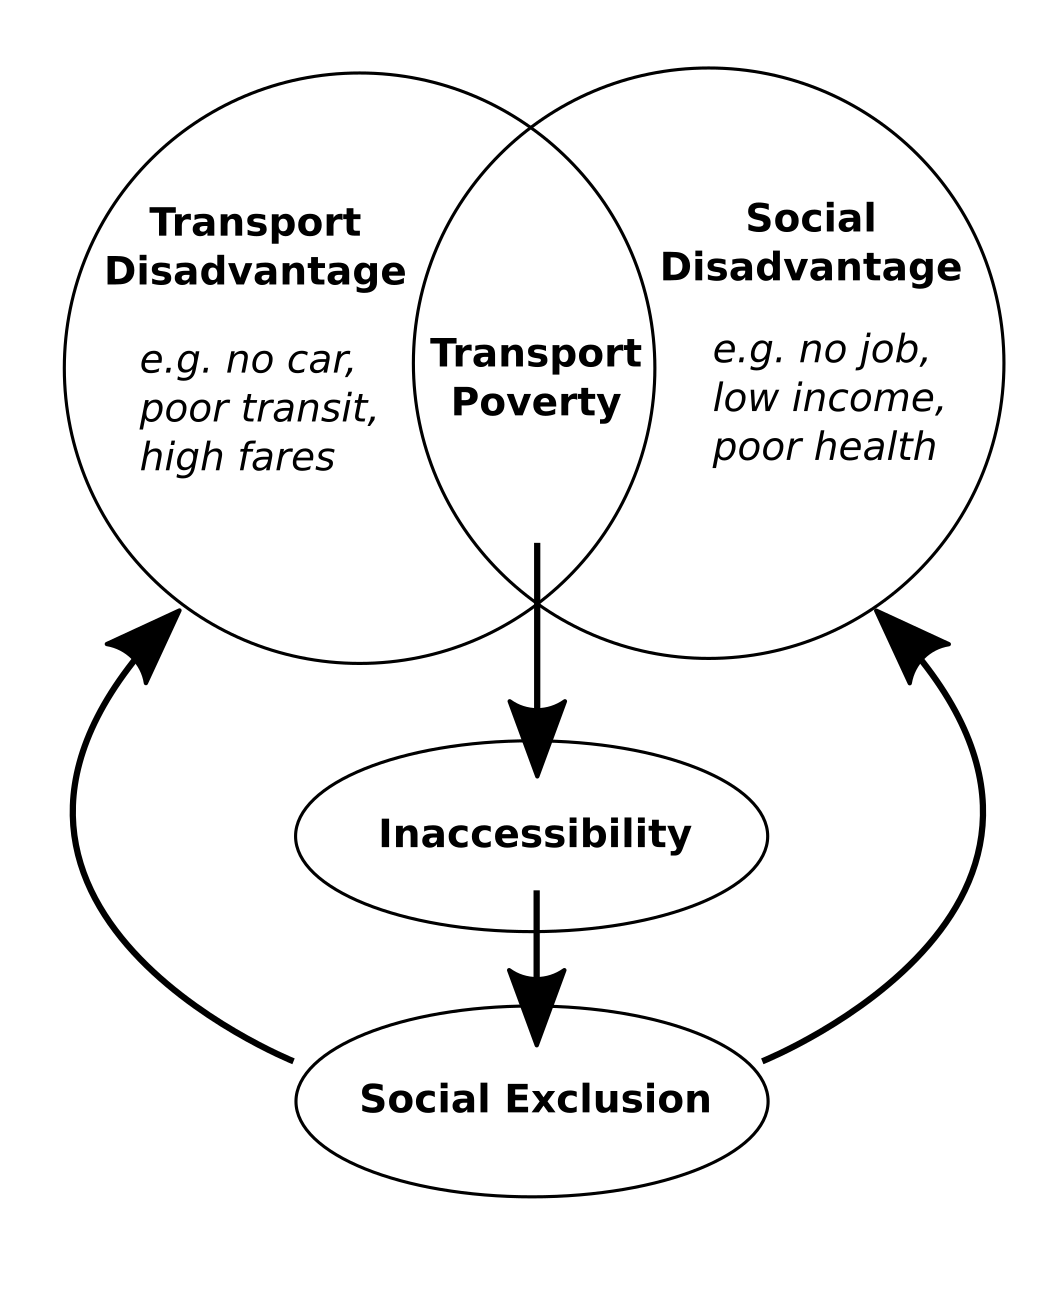
\includegraphics[width=3in]{figures/tpov.png}
	\label{tpov}
\end{figure}

Transport poverty can be heightened in poor neighbourhoods with low levels of accessibility \cite{lucas_is_2018, allen_sizing_2019}. For example, this can occur if jobs in city decline, but poor population does not, many will have to try to find work in the suburbs, increasing commuting costs. This has been termed spatial mismatch \cite{holzer_spatial_1991}. As well, finding employment in suburban areas can be more difficult since search costs are greater, and in some cases, a lack of nearby social services. Moreover, if suburban populations have increased, then wages may decline at suburban job locations since there are more people competing for nearby jobs. If wages are not able to supersede commuting costs, then people will not take these jobs. This can also be compounded with other components of social disadvantage experienced by poor inner-city residents (lack of education, lack of social networks, single parenting, etc.) \cite{holzer_spatial_1991}. It is arguable that this spatial mismatch is becoming inverted, with poverty concentrated in the inner-suburbs but jobs being concentrated in the city centre or dispersed in auto-oriented business parks. Chapter \ref{ch:subtrapov} of this dissertation examines whether, and if so how, both social and transport disadvantage are increasing in more suburban neighbourhoods. i.e. are there trends of a suburbanization of transport poverty







\section{Transport Justice \& Equity}

% tranasport planning and equity

A primary goal of urban transport is to provide people the ability to travel to daily activities in a reasonable amount of time \cite{martens_transport_2016}, and especially to try to reduce the prevalence of transport poverty. If people are not able to travel to activity destinations necessary for their well being it indicates that the transportation network is not fulfilling one of its intended purposes. 

Despite these basic objectives, it has been argued that the traditional paradigm of transport planning is socially regressive \cite{martens_transport_2016}. Transport planning practice was historically based on the observation that aggregate patterns of travel behaviour are the product of supply (of activities) and demand (population) who are limited by constraints (money, mobility, nearby available opportunities) \cite{hanson_determinants_1982,wegener_land-use_2004}.
This historically took the form of four-step travel demand modelling, and in some regions, has evolved into more detailed activity-based micro-simulations \cite{wegener_land-use_2004}. A result of traditional transport planning models is an egalitarian form focused on the network (and usually road and highway networks) rather than individuals. Travel demand models are most often built on revealed preference survey data, and are thus biased towards those groups and individuals who travel more often and further distances. Those who travel less are not considered as much due to the summation on links. Wealthier people tend to drive further distances by car than the poor, and are part of more links on the network model. Therefore, this type of transport planning benefits the rich more than the poor, and thus prioritizing investments in such a way creates further inequalities \cite{martens_transport_2016}.

% 	Planning for equality in mobility by car can be socially regressive. For one, such planning rarely considers people without cars (e.g. because they cannot afford a car, are not physically able to drive, or of age to drive). The result of prioritizing car-based travel can then feedback into encouraging people travelling more by car, if they can, but then further exasperates inequalities between those who can and cannot drive \cite{martens_transport_2016}. It also further abets modal inequalities, prioritizes streets to be focused on the car, and erodes the urban fabric, in which many lower-income people depend. Many urban neighbourhoods were cleaved with highways throughout the 20th century, destroying the communities through which they passed, either directly by evicting people and tearing down housing to make way for the highway, or by fracturing the neighbourhoods adjacent to them \cite{jacobs_death_1961}. 

% planning for accessibility philosophy
As such, several researchers have argued for transport planning to be based on philosophical arguments and theories of social justice \cite{banister_inequality_2018,pereira_distributive_2017,martens_transport_2016}. Development of a theory of justice for transportation has been thought of as a two-step process. First this has involved setting the good of transportation as separate from all other goods (\citeA{martens_transport_2016} argues this via Walzer's Spheres of Justice). Second, this has involved outlining principles of justice that can define and distribute this good. Recent discussion on distributive justice of transport has drawn upon primarily from two philosophical ideas. The first is \textit{Rawls' egalitarianism} \cite{rawls_theory_1971}, that argues that people should have as much freedom as possible, as long as it does not impact other people's freedom (e.g. cars should not limit people's ability to walk in a city). In other words, inequality is only fair if people have equality of opportunity and if policy benefits the least advantaged members of society. i.e. inequality is okay if they stem from preferences, not arbitrary circumstance. Since inequality is inevitable, policy should be based on a \textit{maximin} criterion, that policy should maximize the minimum level of primary goods of the people in the worst-off position \cite{martens_transport_2016}. The Rawlsian approach focuses on goods, such as income. The second, and expanding on the Rawlsian approach, are \textit{Capability Approaches} where the focus should not be on goods, as Rawls' suggests, but on human capabilities. i.e. a focus on the ends (e.g. activity participation), not the means (e.g. income, owning a car) \cite{sen_human_2005}. Reducing capability inequalities will thus increase equality of opportunities. \citeA{martens_transport_2016} and \citeA{pereira_distributive_2017} use this for setting an agenda for transport justice, that we should not be trying to fairly distribute a good (such as income or cars) but instead fairly distribute a capability, and in the context of transport, this capability is accessibility, the ease of reaching activity destinations. They argue that this should be based on setting minimum standards of accessibility to destinations, minimizing inequalities in accessibility, and mitigating transport externalities. 

% what should transport system be?
Many researchers have argued that accessibility benchmarks should be specifically defined in transport planning documents \cite{manaugh_integrating_2015, allen_benchmarking_2019}. In general, accessibility should not be so low that it infringes upon peoples rights, nor should accessibility levels be improved for some if they worsen it for others who already have less. However, it is still an open question of what is an acceptable minimum level of accessibility  (or even how to measure it), and how this varies for different people with varying constraints and capabilities. Accessibility is indeed a combined capability, based on these individual components (e.g. physical ability to ride a bike, income to afford a car, etc.) and the transport-land-use system. Defining sufficient accessibility is difficult, as it requires knowledge of the distribution of existing levels of accessibility and consequences for real people. \citeA{martens_transport_2016} argues this should be based on the relationship between accessibility and activity participation, that likely has a non-linear shape \cite{allen_planning_2020}.  Then the question becomes, what is a fair level of activity participation? Activity participation captures outcomes (what people do), while accessibility captures capability (what people can do). This should be based on the benefits, not just the quantity of activity participation (which is more of a proxy for the quality, but can indicate possible social exclusion).  However, current methods of such are limited to econometric models and travel survey data, and simply counting activity participation by types of activities \cite{fransen_spatio-temporal_2018,allen_planning_2020}. 

%Another uncertainty in defining accessibility thresholds is that even though everyone wants accessibility, they want it to varying extents, and value different flavours of accessibility more or less than others (e.g. some have greater preference for access to jobs, others access to green space, etc.), making sufficient accessibility difficult to define.



\section{Research Gaps \& Motivation}

% relate to urban dynamics
One area to be particular concerned about in transport planning is how the social geographies in cities are changing over time. As I noted in a previous section, the distribution of the low-SES households has shifted from city centres to more suburban locales \cite{ehrenhalt_great_2012,ades_are_2012}. Given these trends of suburbanization of poverty, there are now more low-income households in more suburban areas than in previous decades \cite{ades_are_2012,ades_is_2016,breau_pulling_2018}. This is potentially increasing the risks of transport poverty, and further exasperating urban inequalities more generally. However, it remains unknown how the risks of transport poverty are increasing in cities alongside trends of suburbanization of poverty. Research on neighbourhood socio-economic change has typically not included transport variables like transit accessibility, car ownership, commute times, and activity participation rates - key indicators of transport poverty and its outcomes. There have been a few studies that descriptively examine changes in public transit accessibility over time alongside changes in neighbourhood level socio-economic status \shortcite{foth_towards_2013,farber_transit_2017,deboosere_understanding_2019}. However, these have been predominantly focused on public transit infrastructure, and did not consider car-ownership, an important component of transport (dis)advantage, nor have they considered outcomes such as activity participation. They are also only focused on a short time period or only consider the impacts of specific transit lines, rather than examining region wide changes over periods longer than a decade. There is some research by transportation engineers on analyzing changes in trip and activity rates over longer periods time \shortcite<e.g.>{roorda_two_2008,kasraian_multi-decade_2020,ozonder_longitudinal_2020}. These studies tend to focus on aggregate trends at a regional level or improving the predictive capability of travel demand models, but they provide little insight on the links between travel behaviour with neighbourhood-level demographic changes, increasing income inequalities, and geographies of transport disadvantage. These gaps the literature will motivate Chapter \ref{ch:subtrapov} of this dissertation, which focuses on analyzing and modelling how the geography of activity participation and commute times changes over time, relative to changes in accessibility and urban social geographies.

Chapter \ref{ch:pathsubpov} is particularly motivated by how ample research \cite<e.g.>{ades_is_2016,breau_pulling_2018,grant_changing_2020} has shown trends suburbanization of poverty at regional and neighbourhood levels in Canada, but has been unable to uncover how residents end up to become poor and living in the suburbs. This is because this existing research, as well as the the analysis in Chapter \ref{ch:subtrapov}, focuses on changing neighbourhoods rather than the individuals and households within these neighbourhoods. While there have been studies looking at residential mobility relating to gentrification \cite{freeman_displacement_2005, ding_gentrification_2016, dragan_does_2019, delmelle_new_2020}, little has examined residential mobility pathways to suburban poverty. The objective of Chapter \ref{ch:pathsubpov} is to thus first develop a conceptual framework describing different potential pathways to suburban poverty, and then uses individual-level data to quantify these pathways across urban regions in Canada. This analysis specifically estimates for the first time in Canada to what extent suburban poverty stems from intra-urban residential mobility, external immigration, and remaining poor in-place---thus providing an important link between theory and empirical evidence on the urban dynamics that lead to suburbanization of poverty. Understanding and quantifying the propensities of these pathways will provide important knowledge about the formation of suburbanization of poverty.

Motivation for Chapter \ref{ch:lowinctra} directly stems from how many transit rich neighbourhoods have become more expensive (i.e. gentrifying) and are potentially resulting in the residential displacement and exclusion of low-income residents. This has important social inclusion implications since many low-income residents are reliant on public transit for travelling to daily activities \cite{allen_planning_2020,barri_can_2021}, including finding employment \cite{fransen_relationship_2019,bastiaanssen_does_2021}. Moving away from relied upon public transit could thus decrease capabilities for activity participation, and in some cases, increase risks of transport-related social exclusion \cite{lucas_transport_2012,allen_planning_2020}. However, previous quantitative studies have mixed or inconclusive results about whether low-income residents move disproportionately out of gentrifying neighbourhoods or whether newly built transit infrastructure directly leads to the displacement of low-income residents \cite{rayle_investigating_2015, zuk_gentrification_2018,padeiro_transit-oriented_2019,delmelle_transit-induced_2021}. This existing research that studies income inequalities of residential mobility in relation to public transit has focused only on the outcomes of specific transit corridors and stations, which serve only a fraction of the population in a region, rather than comprehensively examining changes across an entire region. Accordingly, Chapter \ref{ch:lowinctra} analyzes whether there are social inequalities at a regional level pertaining to whether lower-income residents are unequally reducing their levels of transit accessibility when they move. 





\chapter{Suburbanization of Transport Poverty}
\label{ch:subtrapov}


\section*{{Abstract:}}


	Many cities have undergone spatial re-distributions of low-income populations from central to suburban neighborhoods over the past several decades. A potential negative impact of these trends is that low-income populations are concentrating in more automobile oriented areas and thus resulting in increased barriers to daily travel and activity participation, particularly for those who are unable to afford a private vehicle. Accordingly, the objective of this paper is to analyze the links between increasing socio-spatial inequalities, transport disadvantage, and adverse travel behaviour outcomes. This is examined first from a theoretical perspective, and second via a spatio-temporal analysis for the Toronto region from 1991 to 2016. Findings show that many suburban areas in Toronto are not only declining in socioeconomic status, but are also suffering from increased barriers to daily travel evidenced by longer commute times and decreasing activity participation rates, relative to central neighborhoods. Because of these adverse effects, this evidence further supports the need for progressive planning and policy aimed at curbing continuing trends of suburbanization of poverty while also improving levels of transport accessibility in the suburbs.



\section*{{Keywords:}}

transportation, neighborhood change, poverty, daily travel, suburbs








\normalsize




\section{Introduction}

% background
In most early industrializing cities, poverty was traditionally clustered within central areas, while the more affluent lived in peripheral parts of cities away from heavy industry and pollution. During the mid-20th century, many cities have de-industrialized, resulting in increased demand for inner-city living and investment in housing stock in central areas. One effect of this in some cities is that the costs of housing in central areas has increased substantially, causing the spatial distribution of lower-income households to shift to less central, but more affordable, peripheral neighborhoods \shortcite{kneebone_suburbanization_2010,ehrenhalt_great_2012,howell_racial_2014,pavlic_declining_2014,cooke_suburbanization_2015,ades_is_2016}. 

% problem
A potential negative impact of these trends is that low-income households are re-locating to areas that are more auto-oriented, less walkable, and have relatively lower levels of public transit service than central areas. This could be resulting in longer commutes and increased barriers to daily activity participation, especially for those who are unable to afford a private vehicle. The ability to travel to important activity destinations is vital for economic independence (e.g. finding and retaining employment), health, and well-being - and at a greater scale, it can contribute to robust urban economies and healthier societies as a whole. In the worst cases, dissuasion or inability to travel to important destinations can limit activity participation, result in social exclusion, and negatively impact the vitality of urban environments \cite{lucas_transport_2012,martens_transport_2016}.

% research goal and methods
Accordingly, the objective of this paper is to describe the links between increasing socio-spatial inequalities (e.g. de-centralization of low-income households), transport disadvantage (e.g. spatial distribution of zero-car households, low levels of transit accessibility), and adverse travel behaviour outcomes (e.g. lengthier commute times and lower activity participation rates). This is discussed first from a theoretical standpoint with reference to existing research, then a neighborhood level empirical investigation is conducted for the Toronto region, a city that is experiencing growing income inequalities and concentrations of poverty in more suburban areas \shortcite<e.g.>{hulchanski_three_2010,walks_social_2001,ades_are_2012,breau_pulling_2018}.
This exploratory investigation is informed through six periods of the quinquennial Canadian census and a regional travel survey (from 1991 to 2016) in order to describe neighborhood-level changes in socio-economic status (SES) \textit{vis-\`a-vis} changes in transport disadvantage and travel behaviour outcomes. Our methods include computing transit accessibility metrics that are comparable over time, statistical mapping, modelling changes in travel behaviour over time, and visualizing neighborhood change with respect to levels of suburbanization. While focused on Toronto, these methods can be transferable to other regions.

% key results 
The key finding of our analysis is that social and transport disadvantage are increasing more in the suburbs relative to central areas, leading to adverse travel behaviour outcomes such as increasing commute times and lowering activity participation rates. Policy and planning strategies to reduce these negative outcomes should thus focus both on curbing trends of suburbanization of poverty as well as reducing levels of transport disadvantage in suburban neighborhoods. 




\section{Background}


Suburbanization of poverty refers to the spatial re-distributions of low-SES households from central to suburban neighborhoods, usually in reference to changes occurring during the latter half of the 20th century and early 21st century. Recent research has highlighted trends of suburbanization of poverty in early-industrializing cities in nations such as the United States
\cite{kneebone_suburbanization_2010,howell_racial_2014,cooke_suburbanization_2015}, the Netherlands \cite{hochstenbach_gentrification_2018}, Sweden \shortcite{hedin_neoliberalization_2012}, Scotland \cite{kavanagh_is_2016}, and Australia \cite{randolph_suburbanizing_2014}.
% From a research perspective, empirical evidence on suburbanization of poverty is usually based on longitudinal analysis of census data or specific panel surveys analyzing changes in the spatial distribution of low-income households or other SES variables over time.

% Canada
In Canada, there is evidence of increasing income inequalities both within and between regions
\cite{walks_income_2013,bolton_growing_2012,breau_rising_2015,chen_why_2012}, 
% maclachlan_measures_1997
as well as concentrations of low-income households forming in some inner-suburban neighborhoods
\cite{ades_are_2012,pavlic_declining_2014,ades_is_2016,breau_pulling_2018}.
For example, \citeA{pavlic_declining_2014} classified census tracts by density, age of housing stock, and distance to downtown and found that there has been decline or stagnation in prosperity in inner-suburban areas relative to central areas and newer outer-ring suburbs. Research by \shortciteA{ross_dimensions_2004} and \shortciteA{ades_are_2012} computed spatial segregation indices on low-income households and households in poverty in Canadian cities, each finding that economic segregation is increasing at a neighborhood level and that low-income households are becoming increasingly concentrated and isolated within cities' spatial units. Statistical mapping exercises have also highlighted that neighborhoods with higher concentrations of low-income households are located further from the downtown core over the past several decades \cite{ades_are_2012,breau_pulling_2018}.


% concerns
These trends of suburbanization of poverty have raised concerns regarding the increasing polarization and segregation of urban space by class and income \cite{hulchanski_three_2010,walks_income_2013,ades_are_2012}, as well as negative impacts caused by eviction and displacement on individual well-being and disrupted community cohesion \cite{august_challenging_2014,august_its_2016}. There are also increasing concerns that low-income households now have greater levels of transport disadvantage than in previous decades due to being located further from major employment centres and living in neighborhoods with less walkable environments and lower levels transit service, limiting their ability to travel to and participate in daily activities, particularly for those who are unable to afford a private car \cite{skaburskis_filtering_2014,ades_are_2012}. However, the transport-related impacts of suburbanization of poverty remain largely understudied.



% \section{Transport Poverty}

%- overview
A primary goal of urban transport is to provide people the ability to travel to daily activities in a reasonable amount of time \cite{martens_transport_2016}. If people are not able to do so it indicates that the transportation network is not fulfilling its intended purpose. Travel costs are generally felt to a greater degree by lower-income households (e.g. owning or leasing a private car is a luxury that many lower-income households cannot afford). Transport disadvantage (e.g. such as not having access to a car, living in a neighbourhood with low levels of public transit service, etc.) can admix with other forms of social disadvantage (e.g. unemployment, low income, etc.) resulting in negative outcomes like lengthy commutes and barriers to participating in daily activities \shortcite{lucas_transport_2012,lucas_is_2018}. This combined effect is often called transport poverty. This is more likely to occur for lower-SES residents who live in suburban environments as these environments typically have lower levels of transit service and often require the use of private cars, which for many low-income households, are not affordable.

% evidence on transport poverty
Several research projects have empirically analyzed how transport disadvantage can negatively impact activity participation for more at-risk groups like low-income households \shortcite<e.g.>{farber_my_2009,roorda_trip_2010,lucas_modelling_2016,allen_planning_2020}. % casas_social_2007
Auto-oriented environments can also dissuade active transportation like walking or cycling, for example, due to limited or unsafe pedestrian and cycling infrastructure or simply because destinations are too far away \cite{cervero_travel_1997,ewing_travel_2010}. 
While some low-income households that live in suburban environments may be able to afford a car, they are often at greater risk of going into debt because of needing high-interest loans \cite{walks_driving_2018}, being more susceptible to feeling the effects of rising fuel costs \shortcite{mattioli_vulnerability_2019},
% mattioli_vulnerability_2018
and are more likely to drive cars that are used and unreliable, and therefore riskier purchases, despite their lower upfront costs \cite{klein_desperately_2020}. These financial costs of private car access for lower-income households can increase financial stress and cause households to limit spending on other important areas (e.g. housing, healthy food, etc.).

% existing work on estiming where it's a problem - scale, etc.
Accordingly, there have been several recent studies that have analyzed how and where transport disadvantage aligns with socio-economic groups who are more vulnerable to experiencing transport poverty, both in Canada \cite<e.g.>{foth_towards_2013,allen_sizing_2019} and elsewhere \cite<e.g.>{currie_quantifying_2010,fan_impact_2012,dejohn_transit_2019}. 
These studies have either looked at the overall equity of transit systems, for example analyzing whether transit is adequately serving low-SES areas relative to other areas, or have focused on highlighting areas that have high risk of transport poverty; neighborhoods where low-SES households have inadequate public transit service. Generally, transit service is found to be equitable in most cities in the sense that transit is serving neighborhoods with low-SES households relatively more than overall populations. This is unsurprising since lower-income households live in smaller units with higher levels of population density and are more likely to want to live in areas with good transit service due to lack of car ownership. Also, more affluent households generally have less of a preference to live near transit due to being able to afford a car \cite{glaeser_why_2008}.

% discussion with links with sub poverty / neighborhood change
However, given existing trends of suburbanization of poverty, there are now more low-income households in suburban areas than in previous decades in many cities \cite{ades_are_2012,ades_is_2016,breau_pulling_2018}. This is potentially increasing the risks of transport poverty, and further exasperating urban inequalities more generally. However, it remains unknown how the risks of transport poverty are increasing in cities alongside trends of suburbanization of poverty. Research on neighborhood socio-economic change has typically not included transport variables like transit accessibility, car ownership, commute times, and activity participation rates - key indicators of transport poverty and its outcomes. There have been a few studies that descriptively examine changes in public transit accessibility over time alongside changes in neighborhood level socio-economic status \shortcite{foth_towards_2013,farber_transit_2017,deboosere_understanding_2019}. However, these have been predominantly focused on public transit infrastructure, and did not consider car-ownership, an important component of transport (dis)advantage, nor have they considered outcomes such as activity participation. They are also only focused on a short time period or only consider the impacts of specific transit lines, rather than examining region wide changes over periods longer than a decade. There is some research by transportation engineers on analyzing changes in trip and activity rates over longer periods time \shortcite<e.g.>{roorda_two_2008,kasraian_multi-decade_2020,ozonder_longitudinal_2020}. 
% kitamura_formulation_1988, % miller_evolution_2003
These studies tend to focus on aggregate trends at a regional level or improving the predictive capability of travel demand models, but they provide little insight on the links between travel behaviour with neighborhood-level demographic changes, increasing income inequalities, and geographies of transport disadvantage. Accordingly, the goal of the following analysis is to develop deeper understanding of where and to what extent suburbanization of poverty is potentially increasing the risks of barriers to daily travel, in order to better inform policy and planning aimed at reducing these risks. 





\section{Study Area and Data}

The study area for this paper is the Toronto Census Metropolitan Area (CMA). CMAs are agglomerations of municipalities where at least 50\% of the labour force works within the region's core. While not a perfect definition of what counts as an urban region, it is consistent with what has been used in previous research on the Toronto area regarding neighborhood change, socio-spatial polarization, and suburbanization of poverty \shortcite<e.g.>{walks_social_2001,ross_dimensions_2004,ades_are_2012,ades_is_2016}. 
Table \ref{table:summary} indicates how the region has grown from 1991 to 2016, both in terms of population and built-up area.


\begin{table}[h]
	\small
	
	\caption{{Summary statistics of the Toronto CMA from 1991 to 2016}}
	\label{table:summary}
	\begin{adjustwidth}{-1in}{-1in}
		\centering
	\begin{tabular}{lcccccc}
		\hline
		\textbf{}                          & \textbf{1991} & \textbf{1996} & \textbf{2001} & \textbf{2006} & \textbf{2011} & \textbf{2016} \\
		\hline
		Population (millions)                      & 3.84   & 4.19   & 4.50   & 5.02   & 5.49   & 5.82   \\
		Dwellings (millions)                       & 1.35   & 1.46   & 1.60   & 1.77   & 1.96   & 2.10   \\
		Jobs (millions)                                                    & 1.87    & 1.96    & 2.22   & 2.28    & 2.50     & 2.60  \\
		Built Up Area (km\textasciicircum{}2)      & 1,700  & 1,900  & 2,100  & 2,200  & 2,200  & 2,300  \\
		
		\hline 
	\end{tabular}
\end{adjustwidth}
\end{table}

\subsection{Data Sources}

Data for this study draws from the long-form Canadian census and the Transportation Tomorrow Survey (TTS), the largest household travel survey in the region. Both of these surveys are conducted quinquennially, within a few months of each other (the census in May and the TTS in September). This allows for them to be analyzed in concordance with little temporal uncertainty. 

The Canadian census is divided into short-form and long-form versions. The short-form only asks questions regarding basic demographic information, while the long-form asks a wider range of questions including, but not limited to, education, housing characteristics, employment, and immigration. The long-form census is administered to 20\% of households in Canada. However, the mandatory long-form census was not conducted in 2011, when it was replaced by the voluntary National Household Survey (NHS). The NHS has been criticized for its geographically varying response rate, which in some cases is correlated with different socio-economic variables. For completeness, we decide to use the NHS data for our analysis, but results for 2011 should be treated with caution and greater uncertainty than other years used in this study.

The TTS is a 5\% sample of households in the Toronto region \cite{ashby_transportation_2016}. Its focus has primarily been on collecting data for regional travel demand models. We use the TTS for variables pertaining to car ownership, commuting behaviour, and activity participation rates. A limitation of this survey and derived data is that it only pertains to a single weekday. As well, like many travel surveys, there are concerns regarding under-reporting due to proxy responses per household, as well as under-reporting of short trips, trips without a specific destination like short recreational trips, or trips undertaken by active modes such as walking and cycling \shortcite{wolf_trip_2003}. Despite these limitations, the TTS is the largest sample travel survey of its kind in Canada, and has been used as the basis for a number of transport planning studies, including longitudinal analyses \shortcite{miller_evolution_2003,roorda_two_2008,kasraian_multi-decade_2020,ozonder_longitudinal_2020}.

Census and TTS data were acquired as aggregate summaries pertaining to neighborhood sized spatial boundaries. TTS data are linked to Traffic Analysis Zones (TAZ) while census data are linked to census tracts. Some of these boundaries were re-delineated over time because of demographic change. To expedite part of our longitudinal analysis, data from each year and each survey are joined to 2016 census tract boundaries via a population-weighted areal interpolation procedure that minimizes error when boundaries change over time (see \citeA{allen_new_2018} for a description of this process). This data harmonization allows for analysis over a 25 year period from 1991 to 2016 at a consistent set of neighborhood-level geographic units ($n$ = 1,133 census tracts)




\subsection{Measuring Social Disadvantage}

Table \ref{table:census} displays the variables from the Canadian census that are used to form our understanding of neighborhood level socio-economic status. This table provides regional context that is important to note prior to examining intra-regional trends. Variables were selected based on two criteria: 1) they have been used in previous studies that have examined social deprivation in Canada \shortcite{pampalon_deprivation_2009} as well as their relation to transport disadvantage \shortcite{foth_towards_2013, el-geneidy_non-stop_2016, allen_sizing_2019}, and 2) variable consistency across multiple census years.

\begin{table}[h]
	\small
	
	\caption{{Summary of Statistics Canada census SES data for the Toronto CMA from 1991 to 2016}}
	\label{table:census}
	\begin{adjustwidth}{-1in}{-1in}
		\centering
	\begin{tabular}{lcccccc}
		\hline
		\textbf{}                          & \textbf{1991} & \textbf{1996} & \textbf{2001} & \textbf{2006} & \textbf{2011} & \textbf{2016} \\
		\hline
		Population (millions)                      & 3.84   & 4.19   & 4.50   & 5.02   & 5.49   & 5.82   \\
		Average household income (in 2016 CAD) & \$92k   & \$87k   & \$100k   & \$104k   & \$102k   & \$112k \\
		\% who live in low-income households                 & 15\% & 21\% & 17\% & 19\% & 15\% & 18\% \\
		\% who have housing cost 30\% or more of their income & 23\% & 37\% & 29\% & 33\% & 32\% & 34\% \\
		\% of dwellings that need major repairs            & 7\%  & 8\%  & 7\%  & 6\%  & 6\%  & 5\%  \\
		
		\% of families that are single-parent families               & 
		14\% & 16\% & 17\% & 17\% & 18\% & 18\% \\
		\% who immigrated internationally in the past 5 years              & 9\%  & 8\%  & 8\%  & 8\%  & 7\%  & 7\%  \\
		\% who do not have a high school diploma    & 33\% & 31\% & 23\% & 20\% & 17\% & 16\% \\
		\% who are unemployed                              & 9\%  & 9\%  & 6\%  & 7\%  & 9\%  & 8\%  \\
		\hline 
	\end{tabular}
\end{adjustwidth}
\end{table}

The regional trends presented in Table \ref{table:census} indicate relative stability in SES over time at an aggregate level, with some exceptions for specific variables. Looking at income, we see that the average income in the region has increased, but there also has been a slight increase in percent of population in low-income households. This deviation aligns with research showing an increase in income polarization in the Toronto region \cite{hulchanski_three_2010}. Education rates have improved substantially in the region over time, from 33\% of adults not having a high school education to only 16\%. Other less pronounced trends over time include relative decreases in dwellings that need major repairs, immigration, and unemployment while there has been a slight increase in percent of single-parent families. Important to note is that relatively stable proportions over time however indicate growing overall counts of people in each group since the overall population of the region is steadily increasing over time (e.g. the total number of people in low income households in 1991 compared to 2016 nearly doubled). The most notable temporal deviation is for 1996, when a recession in the early 1990s explains worse SES indicators for this year (e.g. higher poverty rate, lower average income, greater percent of income devoted to housing).

We also generate a single indicator of neighborhood level socio-economic status using a Principal Components Analysis (PCA) on the variables presented in Table \ref{table:census}. PCAs are commonly used to develop composite indices \cite{oecd_handbook_2008}, including neighborhood-level measures of socio-economic status  \cite{pampalon_deprivation_2009,cabrera-barona_multiscale_2016}. A PCA reduces these correlated observed variables into independent composite variables. Specifically, the results of a PCA are the eigenvectors of the covariance matrix, ranked by how much variance they explain. We considered having more than one indicator of SES, but we found that the first component of the PCA explained 53\% percent of the variance of the eight variables, while the second component only explained 15\% percent. We term this output first principal component as $SES_{i,\gamma}$. It can be represented as a linear combination of the standard score, $Z_{x,i,\gamma}$, of each input variable, $x$, where $i$ pertains to a census tract and $\gamma$ is the year. All variables from all years were normalized prior to the PCA.


\begin{equation}
{SES}_{i,\gamma} = \sum_x w_x Z_{x,i,\gamma} 
\end{equation}

The factor weights, $w_x$, for each variable, $x$, are displayed in Table \ref{table:pca}. Also displayed is the correlation coefficient between $SES_{i,\gamma}$ and $Z_{x,i,\gamma}$. 




The resulting values of $SES_i$ have a mean of zero and a standard deviation equal to two. Also to note is that it has a negative skew ($\bar{\mu}_3$ = -0.75), meaning that wealthier neighborhoods are more similar to each other in terms of SES, while poorer neighborhoods have greater dispersion. This highlights how the poorest neighborhoods are relatively further from the mean that affluent neighbourhoods. Plots of the distribution of $SES_i$ for each year are shown in Figure \ref{fig:SES_violin}. Overall, there is stability in the average levels of SES over time. The notable exception is 1996 where there is a substantial decline in SES, likely due to the early 1990s recession. The relative consistency in distributions of SES by year is contrary to some previous research highlighting increased polarization over time \cite{hulchanski_three_2010}. This is likely because this previous research has focused solely on income inequalities, rather than a composite index of SES. Summary plots like these also mask spatial variations and changes in spatial patterns over time.


\begin{table}[h]
	\small
	\centering
	\caption{{Results of a PCA of neighbourhood level socio-economic status for the Toronto CMA}}
	\label{table:pca}
	\begin{tabular}{lcc}
		
		\hline
		& $w_x$     & corr($SES_{i,\gamma}, Z_{x,i,\gamma}$)   \\
		\hline
		Logged average household income (in 2016 CAD)  & 0.43 & 0.87 \\
		\% who live in low income households     & -0.45  & -0.92  \\
		
		\% who have housing cost 30\% or more of their income & -0.33  & -0.67  \\
		\% of dwellings that need major repairs    & -0.28  & -0.57  \\
		\% of families that are single-parent families     & -0.38  & -0.77  \\
		\% who immigrated internationally in the past 5 years    & -0.30  & -0.62  \\
		\% who do not have a high school diploma  & -0.21  & -0.43  \\
		\% who are unemployed   & -0.39  & -0.79 \\
		\hline
	\end{tabular}
\end{table}



\begin{figure}[H]
	\centering
	
	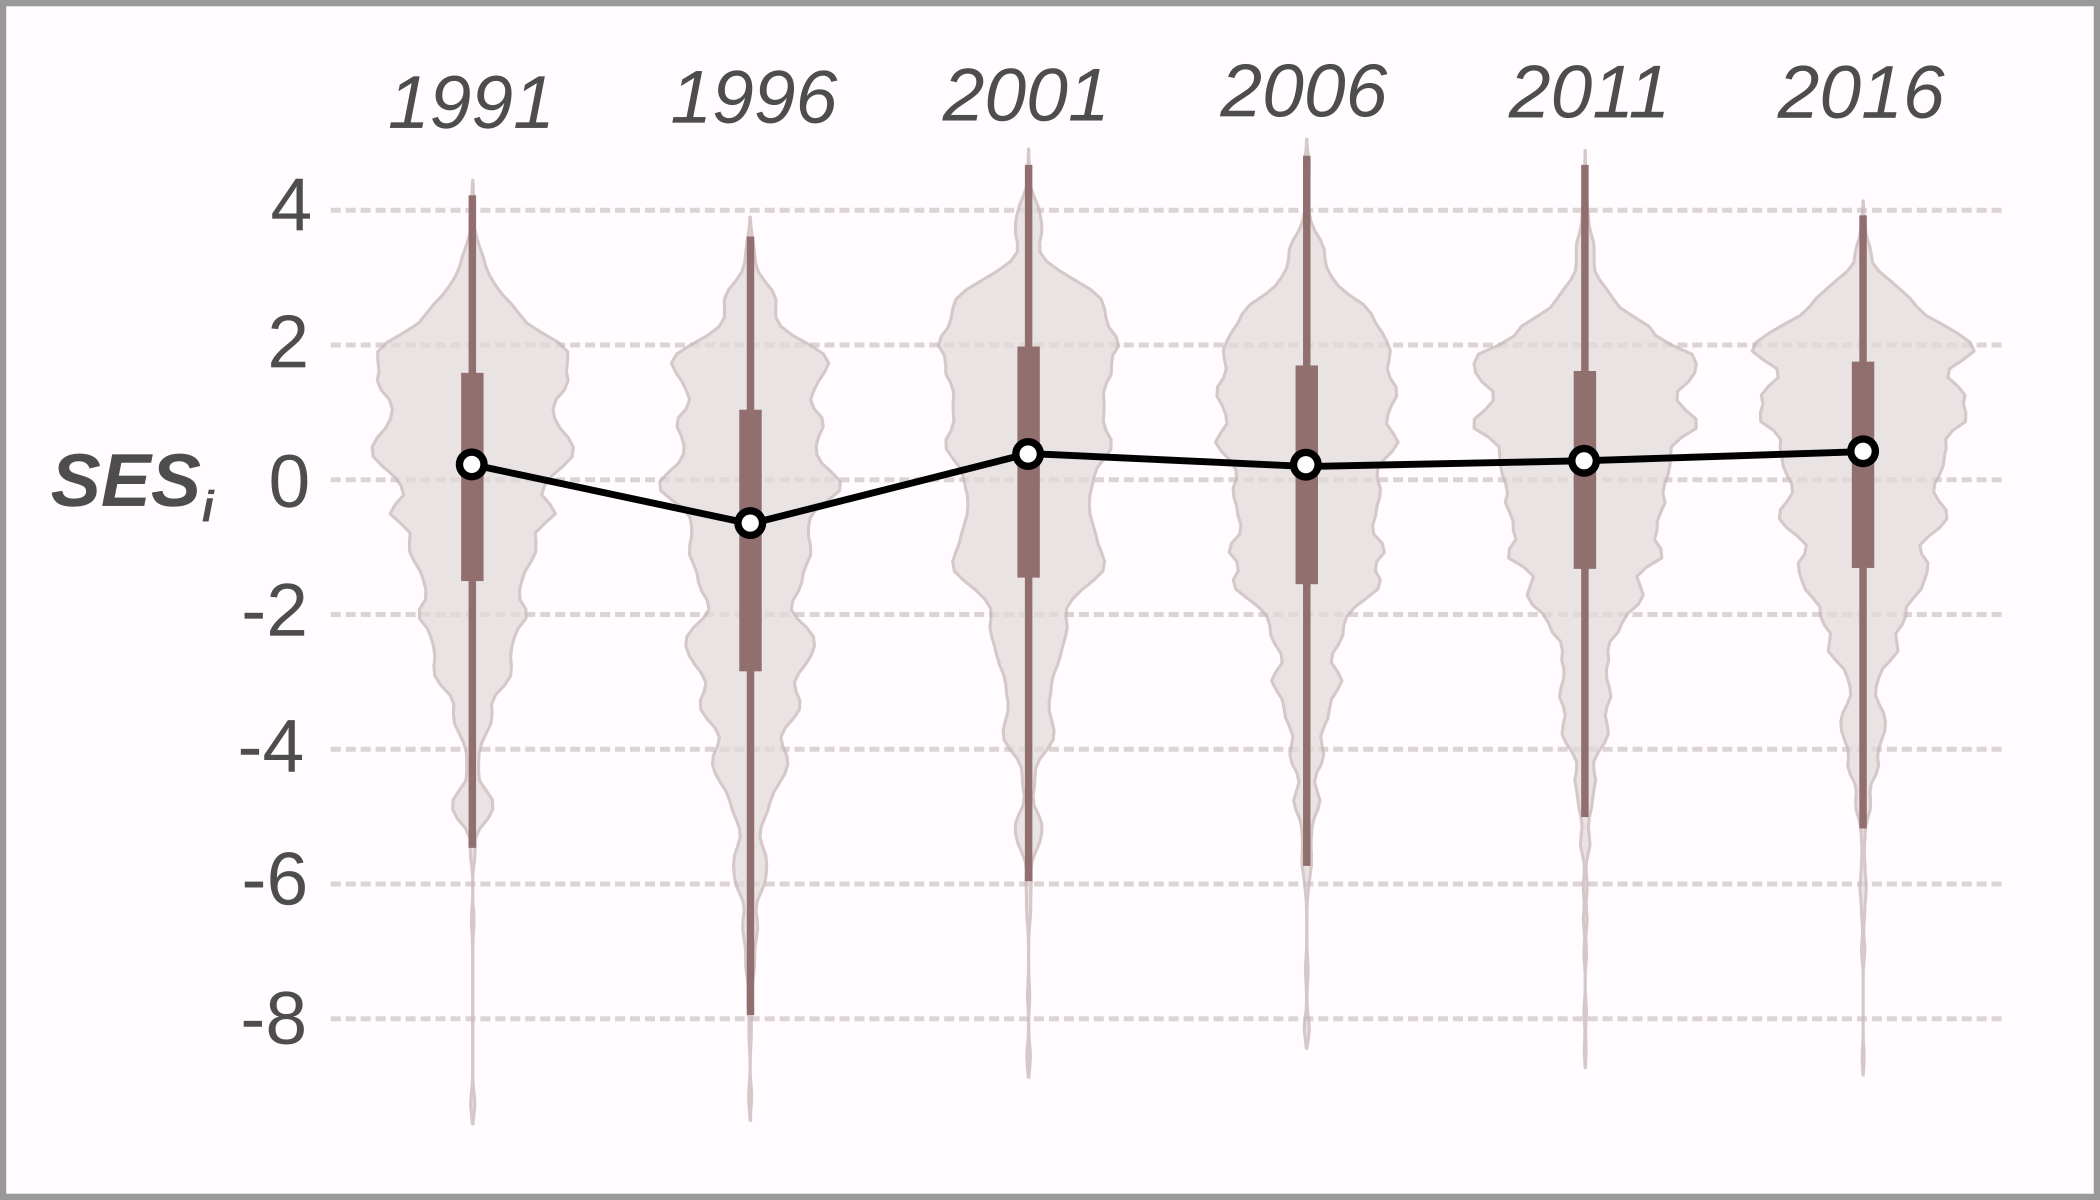
\includegraphics[width=3.5in]{figures/Fig1}
	\caption{{Population weighted distribution in $SES_i$ by year}}
	\label{fig:SES_violin}
	
\end{figure}




\subsection{Measuring Transport Disadvantage}

Transport disadvantage can be considered both in terms of opportunity and outcomes \cite{banister_inequality_2018}. 

For outcomes, we use two travel behaviour variables: activity participation and commute times. Commute times for our analysis are based on historical travel time matrices linked to origin-destination survey data. These travel times were extracted from historical travel demand models of the region for the morning commute period (6:30am to 9:30am) \cite{tmg_gtamodel_2016}. Commute times were averaged by neighborhood. Activity participation is defined as the neighborhood average of the number out-of-home activities people travel to over the course of a day, based on the TTS. At an individual level, the extent of daily activity participation could be a result of preferences or constraints. For example, low levels of activity participation could either be due to not wanting to travel to a destination or due to transport disadvantage (e.g. lack of car access) impeding travel. Moreover, high levels of activity participation may not always be based on choice, but could also be due to the time pressures of working more than one job and balancing household activities. Overall, though, previous research has highlighted how low levels of activity participation predominantly indicates that residents are experiencing barriers to daily travel, and furthermore, has been used as evidence of increased risks of transport-related social exclusion \cite{martens_transport_2016,lucas_is_2018}. For instance, mapping neighbourhood-level "participation deserts" have been used as a transport planning tool to assess which neighbourhoods within are region are suffering the most from transport disadvantage \cite{allen_planning_2020}.  

For opportunity, we consider this in two dimensions as well: transit accessibility and auto availability. For the latter, we compute the percent of households without cars in each neighborhood from the TTS. While it is true that just because a household has a car, it does not necessarily mean that it provides an adequate form of mobility for all members of a household (e.g. there may be competition for its use, and the car itself may not be reliable). However, lack of auto availability has been shown to be a substantial barrier for daily travel within North American urban contexts \cite{blumenberg_car-deficit_2018,allen_planning_2020}, and in the long-term, it is negatively associated with social outcomes such as income and employment \cite{blumenberg_driving_2014,smart_disentangling_2020}. 

Alongside auto availability, we also use the TTS combined with historical travel times to derive place-based measures of transit accessibility in order to describe the quality of public transit service across different neighborhoods. Accessibility is generally understood by transport geographers as how easy or difficult it is for people to reach activity destinations in a reasonable amount of time \cite{hansen_how_1959,geurs_accessibility_2004,el-geneidy_access_2006}. Transit accessibility is also a good proxy for measuring how centralized or suburban a neighborhood is since the greater the level of transit accessibility, the more connected it is to major activity hubs, and the less likely people in a neighborhood are dependent on private cars for daily travel. Relating accessibility to the distributions of populations (e.g. low-income households) can thus also tell us how centralized or suburbanized they are relative to the overall population, and how this may be changing over time. For our study, we compute measures of access to daily non-work activity destinations and access to employment. The first measure can be considered as a general measure of access to activity participation and social interaction in the region. This is calculated as follows:

\begin{equation}
A_{i,D,\lambda} = \sum_{j \in J} D_{j} f(t_{i,j,\lambda})
\end{equation}

$A_{i,D,\lambda}$ is the measure of access to destinations for zone $i$ and travel mode $\lambda$. It can be interpreted simply as the travel-time weighted number of activity destinations reachable from $i$. In the calculation, $D_j$ is the total number of non-work travel destinations in a zone, $j$, $t_{i,j,\lambda}$ is the travel time by mode $\lambda$ from zone $i$ to zone $j$, and $f(t_{i,j,\lambda})$ is an impedance function that weights nearby locations more than those that are further away. We use the same negative exponential impedance function across all study years to allow for comparison over time.

\begin{equation}
f(t_{i,j,\lambda}) = e^{\beta t_{i,j,\lambda}}
\end{equation}

$\beta$ is selected such that the median trip time returns a value of 0.5 with a maximum value of 1 at $t_{i,j,\lambda} = 0$. This selection of an impedance function is based on previous research showing how it can adequately approximate origin-destination trip flows in spatial interaction modelling as well as for its ease of interpretation \cite{osth_new_2016}. Spatial interaction models, specifically doubly-constrained models, include balancing factors which are akin to measures of accessibility. The median non-commute trip duration across all waves of the TTS used in this study (1991-2016) was 15 minutes, resulting in $\beta = -0.0462$. Values of $\beta$ derived for travel demand models in the Toronto region have consistently been within the range of -0.02 to -0.06 \cite{kasraian_multi-decade_2020}.

A measure of access to employment is derived similarly, but it is expanded to also account for the size of the labour force in the region that is competing for employment opportunities. Therefore, this accounts for both job growth and growth of the labour force over time. For example, there are more jobs in the region in 2016 that people can access than in 1991, but there are also more workers in the region competing for these jobs. Measures of accessibility that account for this competition have a basis in doubly constrained spatial interaction modelling, and have been used to analyze accessibility across different spatial contexts \cite{horner_exploring_2004,allen_measure_2020}. This is computed as follows.

\begin{equation}
A_{i,E,\lambda} = \sum_{j \in J} \frac{E_{j}  f(t_{i,j, \lambda})}{L_{j,P}} 
\end{equation}
\begin{equation}
L_{j,P} = \sum_{\lambda \in \Lambda} \sum_{i \in I} \frac{\alpha_{\lambda,i} P_{i}  f(t_{i,j, \lambda})}{A_{i,E,\lambda}} 
\end{equation}

$A_{i,E,\lambda}$ is the access to employment measure for zone $i$ and mode $\lambda$ and $L_{j,P}$ is a measure of access to the labour force. $A_{i,E,\lambda}$ can be interpreted as the number of jobs per worker. $E_{j}$ is the total number of jobs in zone, $j$, and $P_i$ is the number of workers in zone $i$. $\alpha_{\lambda,i}$ is the mode share for travel mode $\lambda$ such that $\sum_{\lambda \in \Lambda} \alpha_{\lambda,i} = 1$. Since $A_{i,E,\lambda}$ and $L_{j,P}$ are dependent on each other, they are estimated in an iterative fashion until they reach convergence. We use the same impedance function, $f(t_{i,j, \lambda})$, described in equation (3), but with a different decay parameter ($\beta = -0.0277)$ that corresponds to a value of 0.5 for a 25 minute commuting trip (the median commute time across all waves of the TTS). % 

The two accessibility measures are then combined into a single index, scaled between 0 (lowest) and 1 (highest). This is partly due to the high correlation between them ($r$ = 0.98), and to streamline the subsequent analysis. Given that both forms of activity participation are theoretically important, we also thought it would be best to combine them, even though just using one would only have a slight variation in terms of any subsequent results.

\begin{equation}
A_{i,\lambda} =  \frac{0.5 A_{i,E,\lambda}}{\max{(A_{i,E,\lambda})}} + \frac{0.5 A_{i,D,\lambda}}{\max{(A_{i,D,\lambda})}}
\end{equation}

Table \ref{table:tts} shows summary statistics of the TTS and the accessibility measures. The percent of zero-car households has remained relatively consistent over time, with a mild peak in 1996 corresponding to the recession. But again, because the population has grown, so has the overall number of zero-car households. Transit accessibility has increased slightly over time. This is indicative that transit service has kept pace with outward expansion, and that inner-city development has occurred in more accessible areas. 


\begin{table}[h]
	\small
	\centering
	\caption{{Summary statistics of transportation metrics from 1991 to 2016 for the Toronto CMA}}
	\label{table:tts}
	\begin{tabular}{lcccccc}
		\hline
		\textbf{}                          & \textbf{1991} & \textbf{1996} & \textbf{2001} & \textbf{2006} & \textbf{2011} & \textbf{2016} \\
		\hline
		
		
		% Jobs (millions)                                                    & 1.87    & 1.96    & 2.22   & 2.28    & 2.50     & 2.60     \\
		% Activity destinations (millions)                                             & 2.39    & 2.42    & 2.79   & 3.07    & 3.55    & 3.25    \\
		\% of households without cars                            & 15.0\%  & 18.0\%  & 16.7\% & 16.6\%  & 14.1\%  & 17.3\%  \\
		Mean transit accessibility ($A_{i,\lambda}$) & 0.33 & 0.35 & 0.37 & 0.37 & 0.39 & 0.37 \\
		
		%Mean access to jobs (transit)                               & 0.41    & 0.42    & 0.44   & 0.44    & 0.46    & 0.45    \\
		%Mean access to activities (transit)                          & 102,100 & 115,000 & 122,000 & 126,000 & 145,300 & 124,800 \\
		%Mean access to jobs (transit / auto)            & 0.29    & 0.31    & 0.32   & 0.30    & 0.32    & 0.31    \\
		%Mean access to activities (transit / auto)  & 0.16    & 0.18    & 0.18   & 0.17    & 0.18    & 0.17    \\
		Mean one-way commute duration (min)                              & 31.0    & 29.8    & 31.4   & 32.0    & 32.3    & 33.2    \\
		%Mean Non-Commute Trip Duration (min)                     & 21.3    & 19.7    & 20.3   & 20.0    & 19.6    & 20.9    \\
		%Mean trips per day                                       & 2.5     & 2.4     & 2.5    & 2.4     & 2.3     & 2.2     \\
		Mean activities per day                                  & 1.39     & 1.32     & 1.37    & 1.31     & 1.30     & 1.20    \\ 
		\hline
	\end{tabular}
\end{table}

In terms of travel behaviour, commute times have remained stable over time, with a slight increase in later years. This aligns with theory that travel time budgets remain relatively stable over time \cite{zahavi_travel_1974,marchetti_anthropological_1994}. Activities per day have decreased over time. This could be due to a number of factors such as changing demographics and preferences (e.g. aging populations travel less, millennials travel less than previous generations, information technology reduces desire for out-of-home activities) \cite{newbold_insights_2018,xu_good_2018}. However, travel barriers could be a factor as well, particularly for the poor who live in auto-dependent neighborhoods.







\section{Analysis and Results}

\subsection{Spatio-temporal Analysis}

Regional statistics like those noted in the previous section do not allow us to examine nuanced spatial changes over time. Accordingly, we map the rate of change of different social and transport variables by neighborhood in order to visually examine where there are growing clusters of change. Specifically, for each variable $x$ we estimate neighborhood-specific linear models as follows:

\begin{equation}
x_i = \alpha_{i,x} + \delta_{i,x} \gamma + \epsilon_{i,x}
\end{equation}

Where $i$ specifies a census tract, $\gamma$ is the year, and $\alpha_{i,x}$, $\delta_{i,x}$, and $\epsilon_{i,x}$ are estimated by ordinary least squares regression. The slope of the line, $\delta_{i,x}$, can be interpreted as the average rate of change of the variable in each neighborhood per year from 1991 to 2006. Such an approach is limited since it does not consider non-linear effects of change over time, but we believe that this is an improvement over simply mapping differentials between two years, which has been common practice in previous Canadian neighborhood change studies \cite<e.g.>{ades_are_2012,hulchanski_three_2010,walks_social_2001}. 

Maps of neighborhood change ($\delta_{i,x}$) are displayed in Figure \ref{fig:change_maps}, and correlations between these rates of change are displayed in Figure \ref{fig:beta_cormod}. 



\begin{figure}[H]
	\centering
	\vspace{-0.2in}
	\hspace*{-0.333in}
	\includegraphics[width=6.5in]{figures/Fig2}
	\caption{{Neighbourhood change in SES and transport disadvantage in Toronto from 1991 to 2016}}
	\label{fig:change_maps}
	
\end{figure}


The top-left panel in Figure \ref{fig:change_maps} indicates where population growth and decline has occurred, with the majority of growth occurring in the suburbs as well as a few pockets of intensification in older urban areas. Areas of population loss have primarily occurred in older, pre-war, neighborhoods just east and west of the downtown core. These neighborhoods have also witnessed the greatest increase in SES, as evidenced in the top-right panel (the correlation between change in population density and change in SES is -0.09). These older centrally located neighborhoods are also often described as those that have undergone gentrification. On the other hand, neighborhoods that have witnessed substantial declines in SES are primarily located in more suburban areas. There is also some growth in low-SES households directly in the city centre. This could be due to a number of factors; increases in post-secondary students, rising housing costs relative to income, or deprivation within social housing and older apartment buildings. Overall, these spatial patterns of changing SES corroborate results of neighborhood change analyses in other research papers \cite{ades_are_2012,breau_pulling_2018,hulchanski_three_2010,pavlic_declining_2014}. 


For car ownership, we observe pockets of zero-car households growing within central and inner-suburban areas. This could be due to high costs of living limiting people's ability to purchase a car, or it could be due to increased preferences to live a car-free lifestyle \shortcite{habib_household-level_2014,papaioannou_study_2020}. Within central areas there are adequate levels of transit accessibility and walkable environments such that having a car is not a necessity. However, it is concerning that carlessness is growing in the inner-suburbs since this could be evidence of a reduction in people's capabilities for daily travel.

Looking at the map of transit accessibility, we see that very few neighborhoods have witnessed a decline in transit accessibility. Most neighborhoods have witnessed no change or achieved increases in transit accessibility. Gains are clearly greatest in the western half of the region. These are areas that have seen some increases in transit service, but also importantly, have witnessed high levels of job growth \cite{blais_planning_2018}, which in tandem has increased accessibility over time. The eastern part of Toronto, known as Scarborough, has not experienced the same levels of job growth nor has it received significant transit investments over the past 25 years, causing a stagnation in transit accessibility over time.


Changes in commute times are less clustered overall but are found more in the periphery. Commute times have increased more in the east, corresponding with transit access stagnation. Activity participation rates also show the greatest declines away from the centre and in areas with decreasing SES. This aligns with both theory on transport poverty \cite<e.g.>{lucas_transport_2012}, as well as empirical research \cite{roorda_trip_2010,allen_planning_2020}, that low activity participation rates are related both to transport disadvantage and SES.


\begin{figure}[H]
	\centering
	\vspace{2mm}
	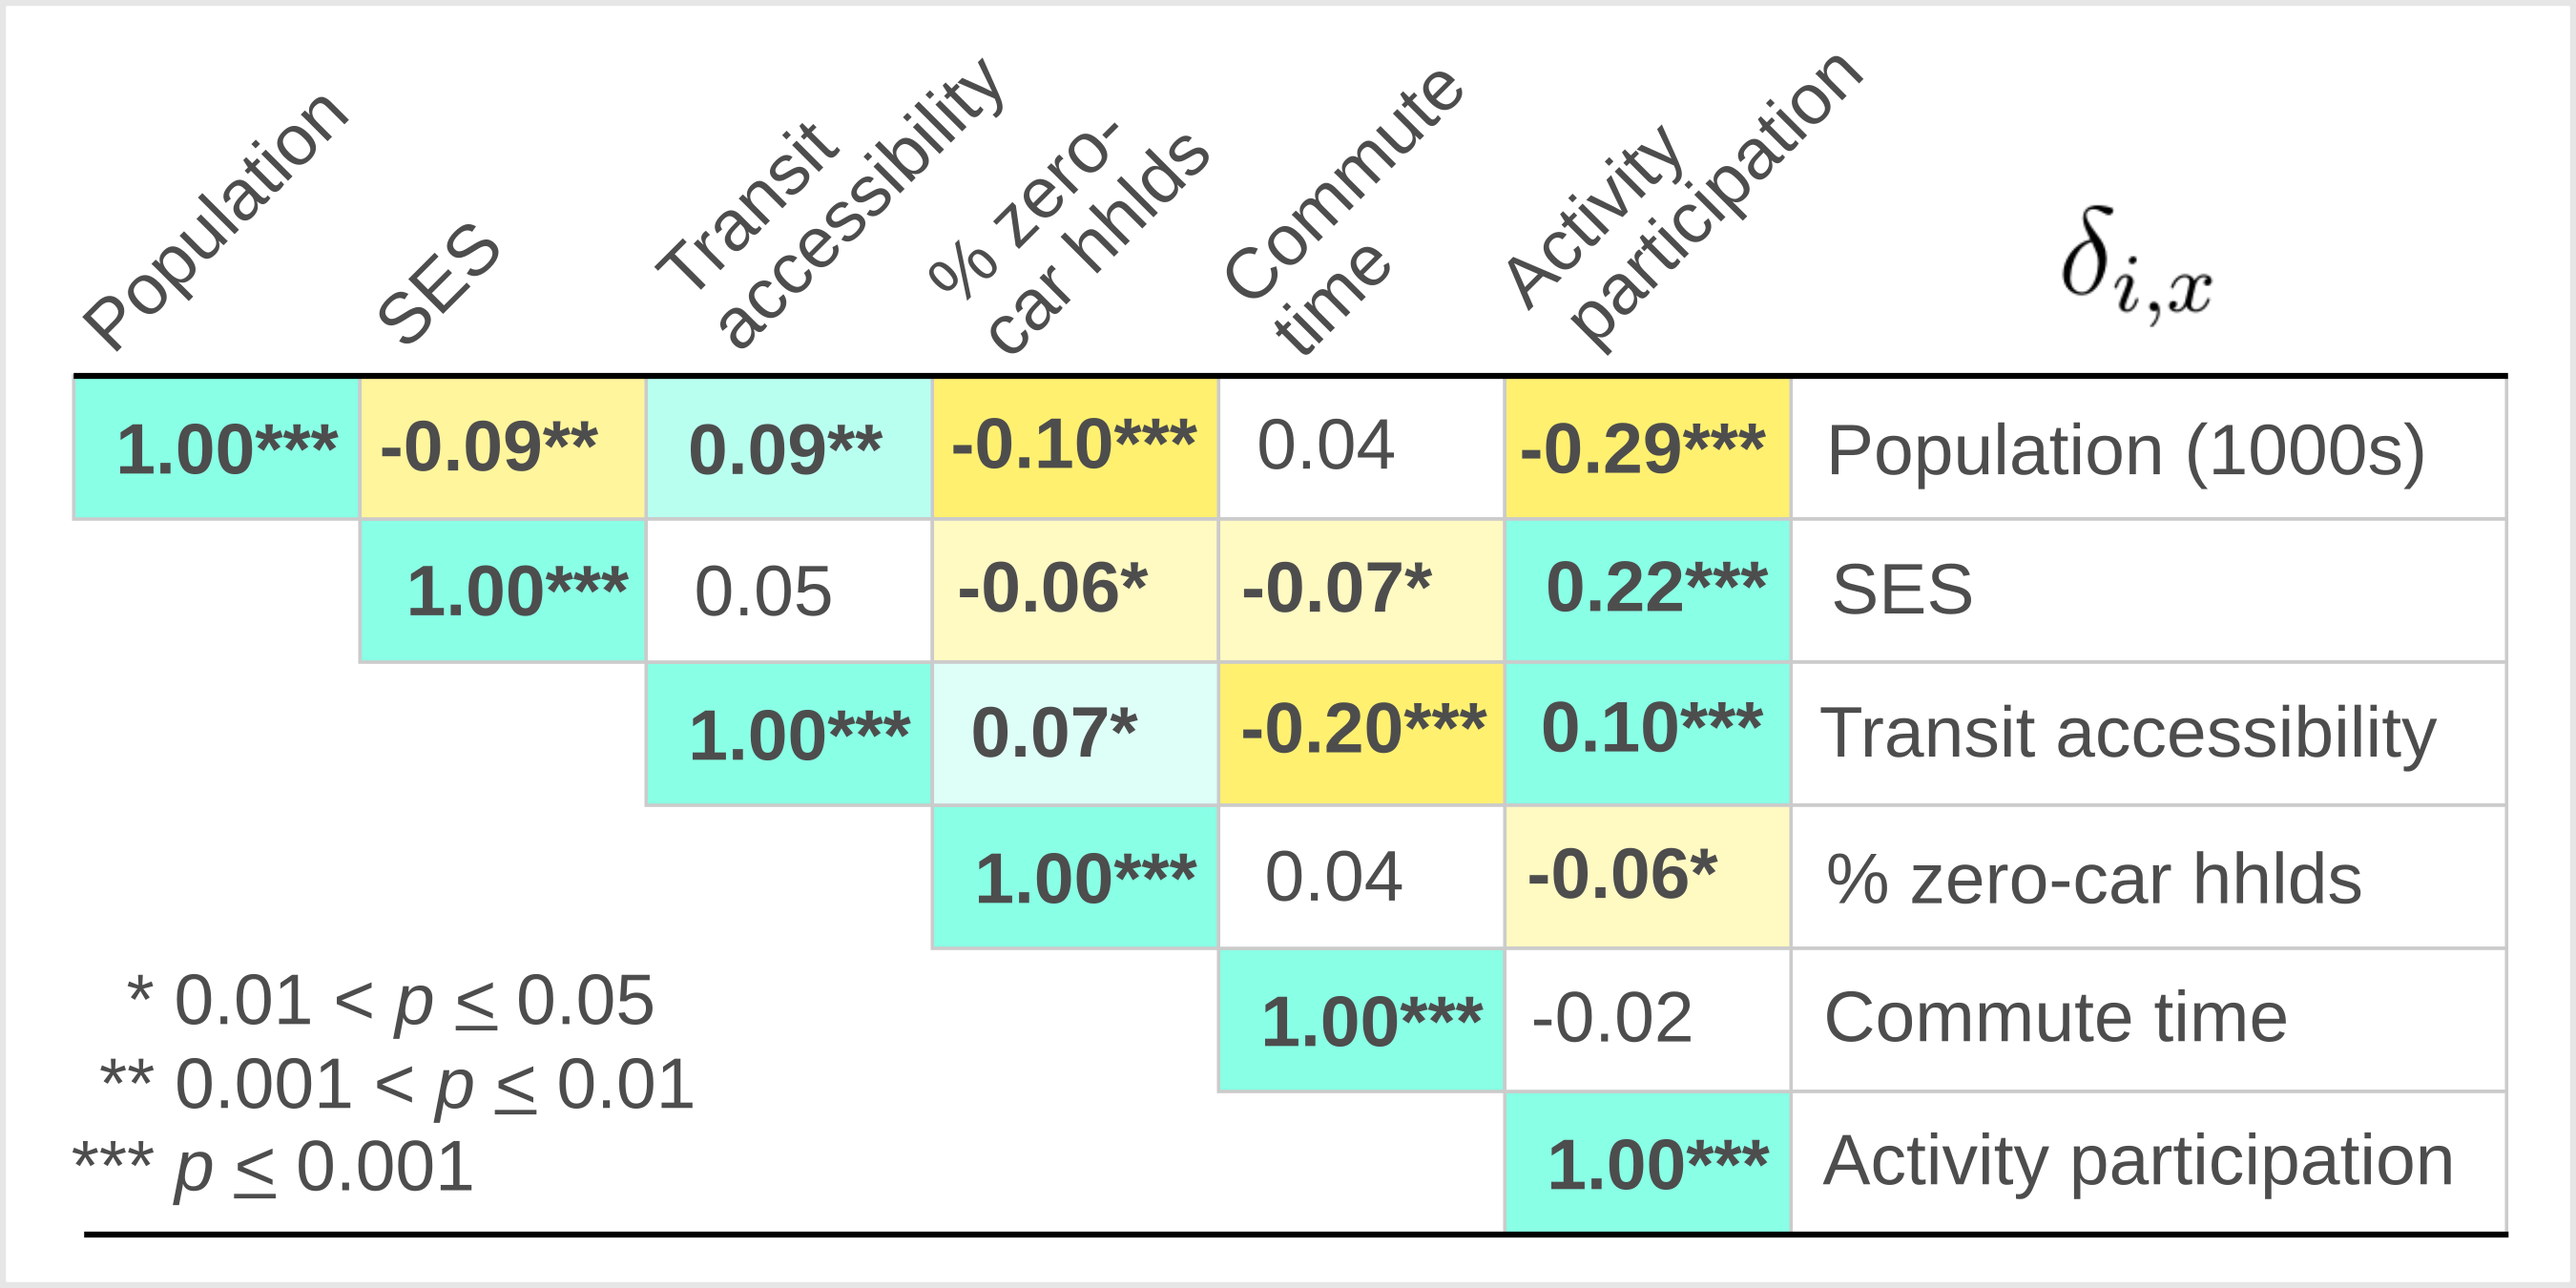
\includegraphics[width=4.5in]{figures/Fig3}
	\caption{{Correlation coefficients between neighborhood change variables}}
	\label{fig:beta_cormod}
\end{figure}


To further explore these relationships, we generate two models to examine the multivariate effects of social and transport disadvantage on adverse travel behaviour outcomes: increasing commute times and declining activity participation rates. These are modelled as follows.

\begin{equation}
Y = \rho W Y + \Theta X + \epsilon
\end{equation}

Where $Y$ is the vector of dependent variables (change in neighborhood averages of commute times and activity participation rates, respectively), $X$ is a matrix of independent variables, $\Theta$ is a vector of coefficients, and $\epsilon$ are the error terms. The models were originally specified using ordinary least squares regression, but we found significant positive spatial auto-correlation among the residuals, leading to specifying a model that incorporates spatial effects \cite{anselin_spatial_1988}. A Lagrange multiplier test was used to decide on using a spatial lag model rather than a spatial error model \cite{anselin_exploring_2005}. This is incorporated via a spatial auto-regressive component, $\rho W Y$, where $\rho$ is a spatial lag parameter and $W$ is a row normalized Queen connectivity spatial weights matrix. Results are displayed in Table \ref{table:model}. In addition to the variables included in the map in Figure \ref{fig:change_maps}, we also included an independent variable representing change in the percent elderly population in each neighborhood since previous research has noted that the elderly travel less than the non-elderly population \shortcite{newbold_travel_2005,xu_good_2018}.


\begin{table}[h]
	\small
	
	\caption{{Model results showing how neighborhood change in social and transport disadvantage effects changes in travel behaviour}}
	\label{table:model}
	\begin{adjustwidth}{-1in}{-1in}
		
		\centering
	\begin{tabular}{lcccc}
		\hline
		& \multicolumn{2}{c}{\textbf{Change in activity participation}} & \multicolumn{2}{c}{\textbf{Change in commute time}} \\
		\hline
		n                & \multicolumn{2}{c}{1133}      & \multicolumn{2}{c}{1133}       \\
		pseudo-R2               & \multicolumn{2}{c}{0.26}      & \multicolumn{2}{c}{0.16}       \\
		\hline
		& \textbf{Coefficient}      & \textbf{\textit{p}-value}         & \textbf{Coefficient}     & \textbf{\textit{p}-value}         \\
		\hline
		$\alpha$ & -0.004           & 0.000     & 0.145           & 0.000     \\
		$\rho$      & 0.400            & 0.000     & 0.388           & 0.000     \\
		Change in population (1000s)      & -0.019           & 0.000     & 0.091           & 0.142     \\
		Change in $SES_i$      & 0.019            & 0.000     & -0.159          & 0.235     \\
		Change in $A_{i,\lambda}$       & 0.281            & 0.003     & -16.250         & 0.000     \\
		Change in \% zero-car households   & -0.002           & 0.002     & 0.044           & 0.013     \\
		Change in \% elderly (65+)  & -0.003           & 0.003     & -0.111         & 0.000    \\
		\hline
	\end{tabular}

	\end{adjustwidth}
\end{table}

The commute time model indicates that increases in transit accessibility and car ownership are linked to reduced commute times, indicating a strong relation to transport disadvantage, overall. Change in SES over time, however, is not found to have a significant association with changing commute times, after controlling for other variables. 


For the activity participation models, we find that growing social and transport disadvantages are both related to declining participation rates. This shows that the fewer resources people have, transport and socio-economic, the less likely they are able to travel to and participate in daily activities. This corroborates previous theoretical and cross-sectional findings on how social and transport disadvantage limit the ability to travel and participate in daily activities, a key indicator of transport poverty \cite{roorda_trip_2010,lucas_transport_2012,lucas_is_2018,allen_planning_2020}. The findings in Table \ref{table:model} show that these trends are also true when examining changes in transport and social disadvantage over time, and lend a somewhat more causal explanation to the observed changes.




\subsection{Suburbanization of Transport Poverty}

In this section, we further examine whether neighborhoods with increasing social and transport disadvantage are occurring more in suburban areas compared to central neighborhoods. To do so, we first need to consider what counts as "suburban". Previous research has used metrics like distance to the urban centre, age of housing stock, and population or housing density, and often result in binary definitions of city versus suburb to describe how centralized or suburbanized a neighborhood is \cite{massey_dimensions_1988,cooke_suburbanization_2015}. Instead, we use our transit accessibility measure to quantify suburbanization, as it is a combination of land-use patterns and connectivity. Transit accessibility is also a predictor of auto-ownership \cite<e.g.>{klein_millennials_2017} and can thus be used to explain how auto-dependent a neighborhood is. Specifically, we take $A_{i,\lambda}$ and average it over the 1991 to 2016 period, $\bar{A}_{i,\lambda}$, as a proxy for neighborhood-level suburbanization. 

We then plot how changes in social and transport disadvantage are related to this accessibility-based level of suburbanization. This is displayed in Figure \ref{fig:sub_pov}. The Y-axes on these plots are values of rates of change from 1991 to 2016 for different variables computed in the previous section. The X-axes are $\bar{A}_{i,\lambda}$ and the legend on the bottom of this figure approximately describes the type of urban form that is associated with different ranges of accessibility. Each dot represents a neighborhood and the curves displayed were fitted via a generalized additive model based on regression splines \cite{wood_smoothing_2016}. The curves describe a moving-window average of how each variable has changed over time for different levels accessibility.

\begin{figure}[H]
	\centering
	\vspace{2mm}
	\hspace*{-0.333in}
	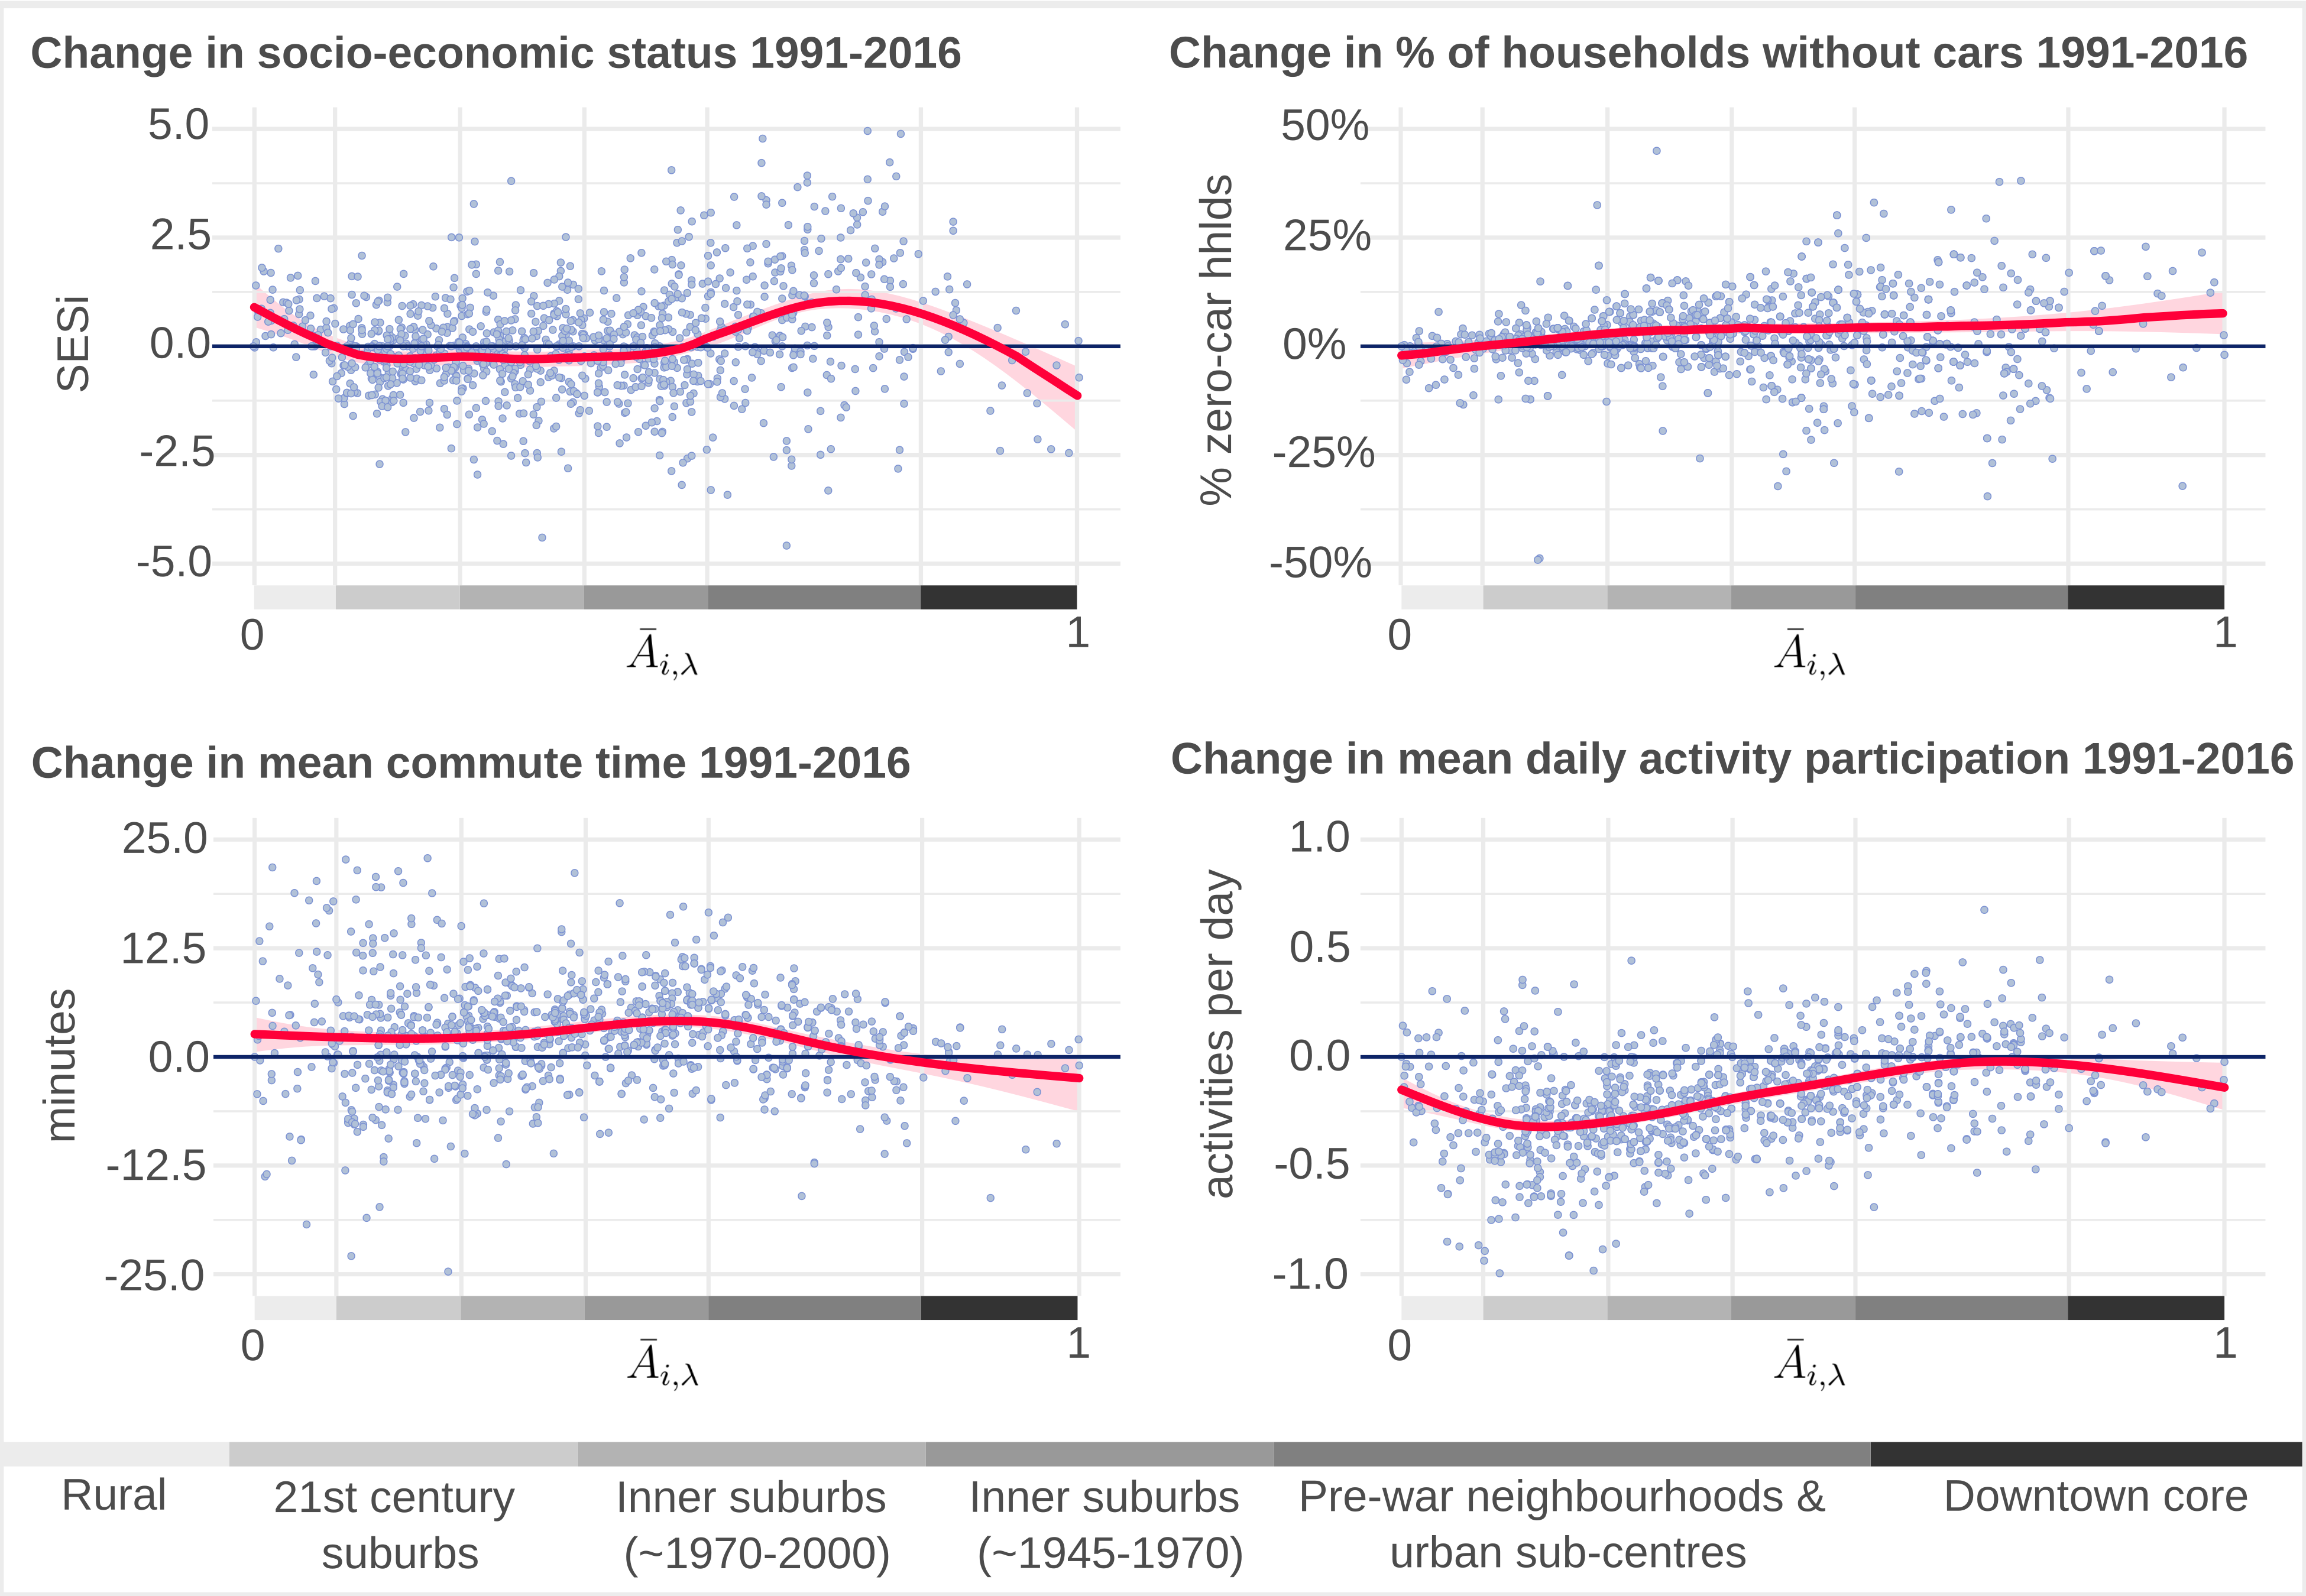
\includegraphics[width=6.5in]{figures/Fig4_sub_plot_4.png}
	\caption{{Change in SES, car ownership, and travel behaviour in Toronto by an accessibility-defined measure of urban form}}
	\label{fig:sub_pov}
\end{figure}

The top-left of this figure shows change in SES by neighborhood. We find that pre-war neighborhoods have substantially improved in terms of SES and that suburban neighborhoods have on average slightly declined in terms of SES. This confirms previous research that has highlighted trends of gentrification occurring close to the core and a decline or stagnation in SES in many suburban neighborhoods \cite{ades_are_2012,hulchanski_three_2010,walks_social_2001,ades_is_2016}. The top-right shows that zero-car households have increased relatively evenly throughout the spectrum of urban structure, with the greatest increase occurring in the downtown core, where there are the highest levels of transit accessibility. The downtown core has also experienced the greatest increase in housing costs over this 25 year period.

Looking at the bottom two plots on changes in travel outcomes over time, we find that commute times have increased more within suburban areas, with a small bump particularly within the inner-suburbs. Only central neighborhoods have witnessed a reduction in commute times on average. Activity participation rates have declined overall, but we observe that this decline is occurring predominantly in suburban neighborhoods. Suburban areas are thus experiencing the brunt of increasing adverse travel behaviour outcomes in the region.

Transport poverty has been described as the compounding of both social and transport disadvantage \cite{lucas_transport_2012, lucas_is_2018}. Accordingly, for our last piece of analysis, we generate a composite measure for examining the extent to which neighborhoods are increasing or decreasing signs of experiencing transport poverty, $\delta_{TP,i}$, and then visualize it's spatial distribution. In particular, we are interested in whether transport poverty is increasing more within the suburbs than central neighborhoods. To generate $\delta_{TP,i}$, we sum the standard scores of $\delta_{i,x}$ for five pertinent variables $x$: change in socio-economic status ($SES_i$), transit accessibility ($A_i$), percent zero-car households, mean commute times, and mean daily activity participation rates. 

\begin{equation}
\delta_{TP,i} = \sum_x \frac{\delta_{x,i} - \mu_{\delta_{x}}}{\sigma_{\delta_{x}}}
\end{equation}

The signs of each $\delta_{i,x}$ are set that positive values of $\delta_{TP,i}$ can be interpreted as neighborhoods with increased travel barriers and worse travel behaviour outcomes over time. Conversely, negative values of $\delta_{TP,i}$ can be interpreted as neighborhoods where signs of transport poverty are decreasing over time, on average. Figure \ref{fig:tpov} visualizes the spatial distribution of $\delta_{TP,i}$ (right) as well as plots $\delta_{TP,i}$ relative to mean levels of transit accessibility $\bar{A}_{i,\lambda}$ (left).

We observe that transport poverty is decreasing substantially in older, centrally located, neighborhoods; gentrifying neighborhoods with salutary levels of transit accessibility and walkable built environments. Conversely, more auto-oriented suburban neighborhoods, on average, are witnessing increases in risks of transport poverty over time. There is, however, quite a bit of variation across this spectrum of urban form. The orange and red areas on the map are those in which transport poverty has increased substantially from 1991 to 2016. Clearly this has occurred in inner-suburban neighborhoods in the east (primarily in Scarborough), as well as more distant suburban areas to the east, north, and northwest. However, this is not to say that all suburbs follow this trend, there are still a number of suburban neighborhoods showing signs that transport poverty is declining over time. These tend to be a combination of neighborhoods where SES has not declined and neighborhoods where transit accessibility has improved. This is particularly evident in the western suburban areas that have witnessed improvements in transit accessibility. Overall, the key finding here is that risks of transport poverty are increasing more within auto-oriented suburban areas than compared to centrally located neighborhoods. 


\begin{figure}[H]
	
	\centering
	
	
	\hspace*{-0.333in}
	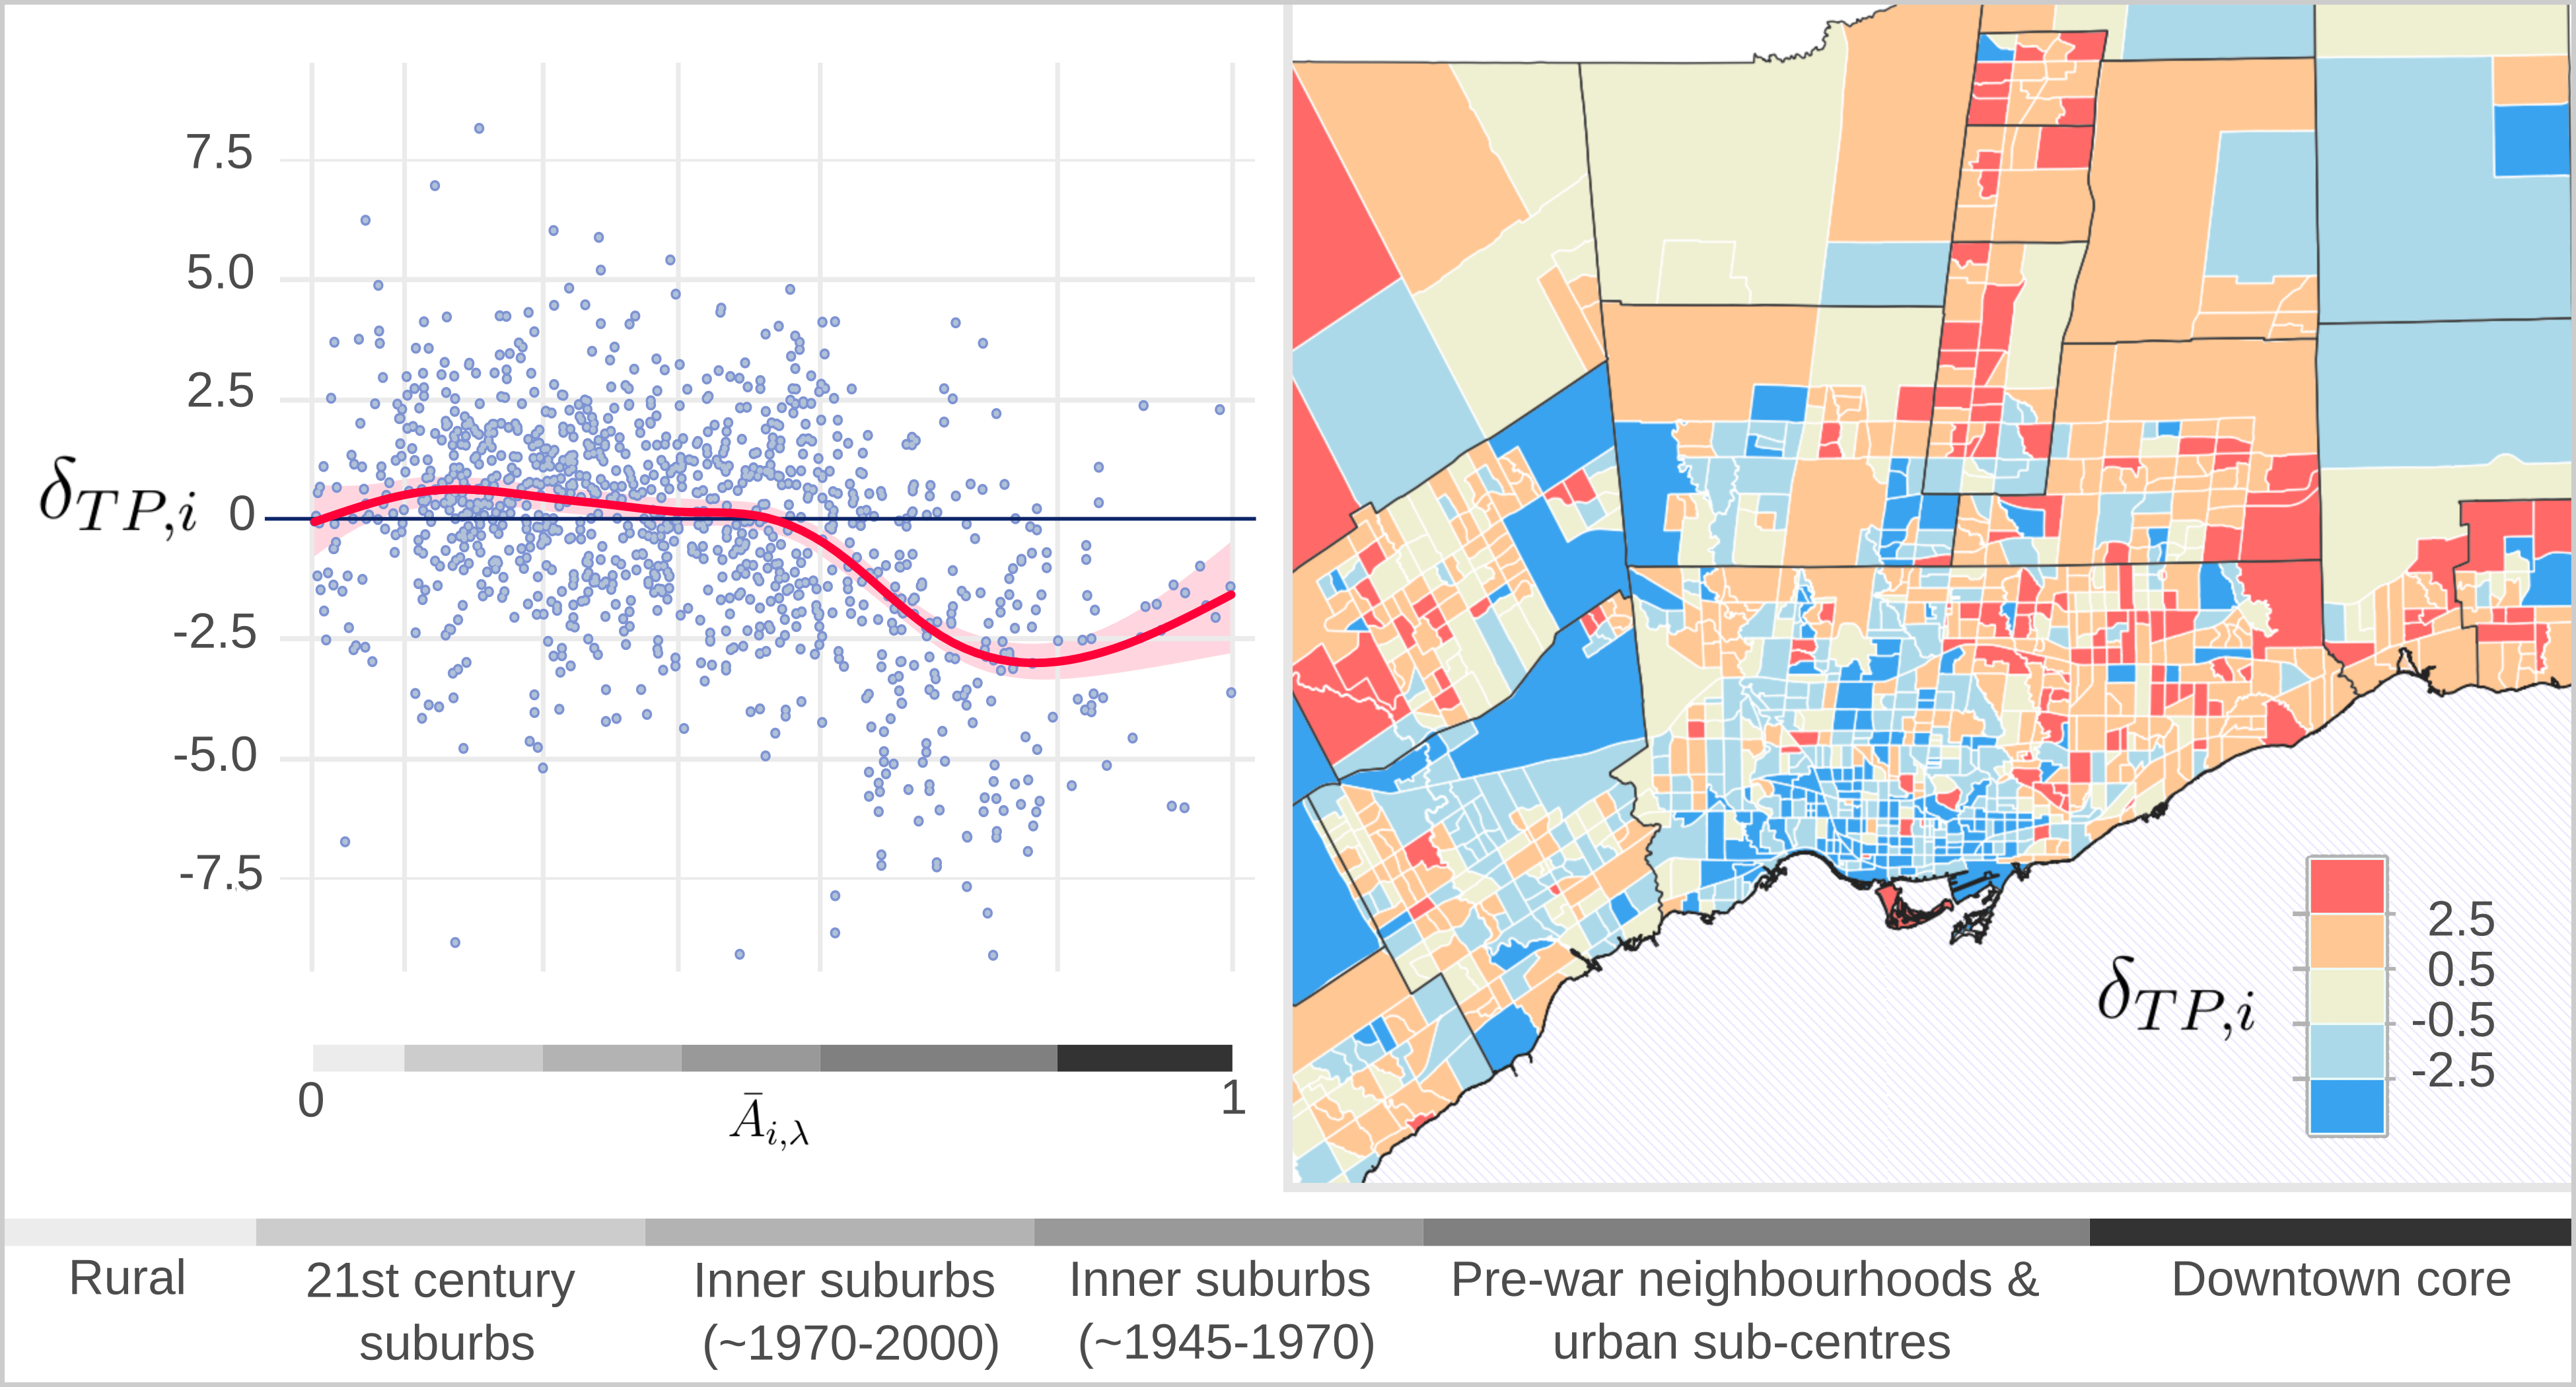
\includegraphics[width=6.5in]{figures/Fig5_tp_time.png}
	
	
	\caption{{Change in transport poverty, $\delta_{TP,i}$, by mean level of accessibility (left). Map of change in $\delta_{TP,i}$ (right).}}
	\label{fig:tpov}
\end{figure}



\section{Conclusions}

% limitations
Our study was not immune to limitations, and thus offers directions for future work. For one, our research focused on transport (dis)advantage in terms of transit access to destinations and auto ownership, but we did not consider other components of urban form that could either benefit or detriment urban living. For example, despite gains in transit access, suburban built environments typically remain focused on the car, which have a number of safety and environmental concerns (e.g. speed limits are greater, safe crossings are more spread out, creating barriers to active travel). On the other hand, some suburban areas offer better access to green space, which can have a positive effect on health and well-being. Future research should consider other positive and negative environmental impacts of less-centralized urban living for low-SES populations. This could prove challenging, however, since there is little readily available historic data on urban form, walkability, and access to green space.

Our study also had some other data limitations. We relied on a travel survey that represented a 5\% sample of the population, limiting analysis at smaller geographic scales. Secondly, there may have been some inconsistencies with how data were collected across survey years. We did select variables that were consistently defined over time based on survey documentation, but there were likely some imperfections in interpretation and administration of survey questions. As well, in terms of data, there was likely some inaccuracy caused by the data harmonization process of apportioning data to the same spatial units. These issues are unavoidable when dealing with longitudinal survey data that has been aggregated to different areal units \cite{allen_new_2018}. 

As well, our neighbourhood-level analysis could be masking individual effects since we only analyzed change at a neighborhood level. For example, there could be more extreme levels of travel be outcomes in later years than earlier years in certain neighborhoods. However, the data are limited in that specific individuals are not tracked over time, preventing the possibility of a true individual-level panel study. These problems highlight the need in the future for individual-level linked datasets, similarly to how medical records have been linked to census data in health research. Analyzing individual panel data would be helpful for examining pathways to suburban poverty and whether improvements in transit accessibility are either more likely to alleviate poverty or result in gentrification and displacement.

Despite these limitations and important directions for future work, our study provides solid evidence that transport poverty in Toronto is increasing more in the suburbs relative to central areas. Eastern suburbs in particular have suffered the most, indicative by having the greatest combination of increased transport and social disadvantage, and evidenced by increasing commute times and declining daily activity participation rates. Our research thus confirms theoretical pathways of transport poverty \cite{lucas_transport_2012}, and moreover, shows that it is occurring more within suburban neighborhoods.

Policy to reduce these effects should thus have a two-pronged approach. The first is to curb the growth of suburban poverty through focusing on increasing the supply of affordable housing in areas with high transit accessibility, having strong rent controls, and preventing forced eviction and displacement from central to suburban neighborhoods. The second is to upgrade suburban environments through transport planning and urban design strategies that improve transit accessibility and walkability (i.e. improving accessibility at both neighborhood and regional scales). These are not new ideas. Many of them have been advocated for previously in terms of reducing the negative population health and environmental impacts associated with auto-oriented environments \shortcite{cervero_travel_1997,ewing_relationship_2003,ewing_compactness_2015}, and limiting the detrimental impacts suburbanization of poverty has on increasing polarization and segregation of urban space as well as the negative impacts caused by eviction and displacement on individual well-being and community cohesion  \shortcite{hulchanski_three_2010,ades_are_2012,walks_income_2013,august_challenging_2014,august_its_2016}. Our research provides one more important piece of evidence showing that such strategies would also be progressive options in reducing barriers to daily travel and transport-related social exclusion.








\section*{3.A \hspace{1mm} Appendix}
\addcontentsline{toc}{section}{3.A \hspace{1mm} Appendix}

\subsection*{3.A.1 \hspace{2mm} Selection of distance decay parameters for measuring accessibility}
\addcontentsline{toc}{subsection}{3.A.1 \hspace{2mm} Selection of distance decay parameters for measuring accessibility}


For our accessibility measures, we used a negative exponential impedance function in order to weight nearby destinations more than those further away (see Section 3.3). This was defined as follows:

\[f(t_{i,j}) = e^{\beta t_{i,j}}\]

Where $t_{i,j}$ is the travel time and $\beta$ is a decay parameter. As we noted in the main text, we followed the advice by \citeA{osth_new_2016} that $\beta$ can be approximated by selecting the curve which returns 0.5 for the median travel time. This is based on their argument that such a selection can adequately approximate origin-destination trip flows in spatial interaction modelling as well as for its ease of interpretation \cite{osth_new_2016}. This led to the selection of $\beta = -0.0277$ for access to jobs and $\beta = -0.0462$ for access to non-work destinations

To further assess the validity of this selection of $\beta$, we first looked at previous research which has measured accessibility over multiple time periods in the Toronto region. There are four studies that we are aware of. The first, by \citeA{foth_towards_2013} claims to use a gravity-based formulation to measure access to jobs. Unfortunately, they do not describe how this function is defined. Two papers, one by \citeA{farber_transit_2017} and the other by \citeA{deboosere_understanding_2019} use cumulative measures of accessibility in their analysis. Cumulative measures are less theoretically sound than those which use continuous decay functions as they over-simplify what is accessible by use of a single isochrone. Most applicable to our study is a recent paper \citeA{kasraian_multi-decade_2020} who select a $\beta$ value of -0.05 when measuring access to population in the Greater Toronto and Hamilton Area. \citeA{kasraian_multi-decade_2020} derive this value of $\beta$ from another rule of thumb \cite{batty_proximate_1984}, where $\beta$ is equal to one divided by the mean travel time (20 minutes was the mean travel time for all trips selected for use in their study). They also justify their selection based on that "travel time parameters in operational travel demand models for the region have consistently fallen within the 0.02–0.06" range \cite{kasraian_multi-decade_2020}. For our study, initially based on the advice from \citeA{osth_new_2016} we used a $\beta$ value of -0.0277 for access to jobs and -0.0462 for access to non-work destinations. These both fall within this -0.02 to -0.06 range. Moreover, if we followed the 
\citeA{batty_proximate_1984} approximation used by \citeA{kasraian_multi-decade_2020}, our values of $\beta$ would be -0.0316 (difference of 0.0039) for access to jobs, an -0.0505 (difference of 0.0043) for access to non-work destinations. These are very close to our selected values.

For the sake of sensitivity, we computed access to jobs using $\beta$ values of 0.02, 0.03, 0.04, 0.05, and 0.06 to show the similarity in results across this range. Below is a correlation matrix of the resulting accessibility measures.

\begin{table}[h]
	\vspace{2mm}
	\small
	\centering
	\caption{Correlation among measures of access to jobs by transit for different values of $\beta$}
	\label{table:beta_cor}
	\begin{tabular}{llllll}
		\hline 
		$\beta$  & -0.02 & -0.03 & -0.04 & -0.05 & -0.06 \\
		\hline
		-0.02 & 1.000 & 0.985 & 0.950 & 0.903 & 0.850 \\
		-0.03 &       & 1.000 & 0.989 & 0.960 & 0.921 \\
		-0.04 &       &       & 1.000 & 0.991 & 0.967 \\
		-0.05 &       &       &       & 1.000 & 0.993 \\
		-0.06 &       &       &       &       & 1.000   \\ \hline 
	\end{tabular}
\end{table}

Clearly there is quite high correlation among these measures, and selecting any value within this range (-0.02 to -0.06) would likely have only very minor differences in results, particularly since we were primarily concerned with relative changes in accessibility over time, rather than absolute values at a particular point in time. 

Furthermore, we also fitted negative exponential curves based on the distribution of trips by their travel times (at minute-by-minute intervals). We did this for the two types of trip purposes and subsequent accessibility measures that we generated, for home-to-work trips ($\beta_W$), and for trips to non-work activity destinations ($\beta_{NW}$). The resulting values are shown below.

\begin{table}[h]
	\vspace{2mm}
	\small
	\centering
	\caption{Values of $\beta$ fitted from travel survey data for Toronto}
	\label{table:beta_fit}
	\begin{tabular}{lll}
		\hline
		Year & $\beta_{W}$ & $\beta_{NW}$ \\ \hline
		1991 & -0.0269   & -0.0389       \\
		1996 & -0.0255   & -0.0464       \\
		2001 & -0.0272   & -0.0399       \\
		2006 & -0.0325   & -0.0426       \\
		2011 & -0.0312   & -0.0521       \\
		2016 & -0.0279   & -0.0486       \\
		All$^*$  & -0.0289   & -0.0432      \\ \hline \\
	\end{tabular}
	
	$^*$All years combined before fitting
\end{table}

We find that each of these values is within a range of less than 0.01 of the $\beta$ values used in our analysis. Extrapolating from our correlation noted above, it is unlikely that selecting one of these fitted $\beta$ values will result in an accessibility measure that is substantially different from what we used. In fact, when looking at the correlations between accessibility measures only 0.01 apart, they are all above 0.98.

To conclude, we believe our selection of $\beta$ is appropriate for our analysis given precedent in the literature, fitted values from data, correlation between accessibility measures, and comparing with the range of values that have been used in previous studies (-0.02 to -0.06). 

Overall, the goal of our study was focused more on the application of accessibility alongside several other socio-economic and transport-related variables to study suburbanization of poverty, rather than specifically and solely focused on developing accessibility measures. Nevertheless, we do think that more work could be done in the future to derive more accurate accessibility measures that are suitable for longitudinal analyses. Clearly our paper, and some of the other papers that we cited above, would benefit from such work to move beyond these relatively simplistic approximations. Doing so would require additional thought about how to appropriately work with matrices from multiple time periods, multiple travel modes, changes in infrastructure, and different sample sizes when fitting spatial interaction models.





\chapter{Pathways to Suburban Poverty}
\label{ch:pathsubpov}


\section*{{Abstract:}}


	Suburbanization of poverty is a concerning trend in many urban regions. While research has described patterns of suburbanization of poverty at regional and neighbourhood levels, there are open questions about how lower-income households have agglomerated in the suburbs in recent history. Is suburban poverty primarily a result of 1) residential sorting within cities of low-income residents from central to suburban neighbourhoods (e.g. gentrification and displacement), 2) patterns of immigrant settlement in cities directed towards the suburbs, or 3) becoming and remaining poor while staying in the suburbs? The objective of this paper is to describe and quantify the propensity of these predominant individual geographic pathways of being poor and living in the suburbs. We do so via a cluster analysis of census and land-use data to define typologies of suburban neighbourhoods and then link this categorization to a large-scale panel dataset representing 20\% of tax filers in Canada (from 2006 to 2016). These data allow for analyzing how different pathways are observed within the context of large Canadian cities, specifically to what extent poverty in suburban neighbourhoods stems from intra-urban residential mobility, external immigration, and becoming poor in-place. We find that becoming poor while staying in the suburbs encompasses a greater proportion of suburban poverty than immigration and centre-to-suburb residential mobility combined. Overall, this research provides insight into the changing structure of urban neighbourhoods while also providing pertinent information to aid preventative policy aimed at reducing suburban poverty in Canada.
	


\section*{{Keywords:}}

suburbs, poverty, residential mobility, immigration, panel data



\section{Introduction}

Many urban regions have witnessed inner-city gentrification and growing concentrations of poverty in the suburbs over the past several decades \cite{ehrenhalt_great_2012,ades_are_2012,grant_changing_2020}. These trends have led to concerns of polarization and segregation of urban space by class and income \cite{hulchanski_three_2010}, negative impacts caused by gentrification and displacement on individual well-being \cite{elliott-cooper_moving_2020}, low quality of low-income housing in the suburbs \cite{august_gentrification_2018}, and that living in auto-oriented suburban environments can reduce accessibility and the ability to travel to daily activities \cite{allen_planning_2020}, which can further compound poverty in suburban areas \cite{lucas_transport_2012}.

Ample research has described trends of suburbanization of poverty at regional and neighbourhood levels, for example by mapping neighbourhood changes in income or poverty rates, and showing how poverty is increasing in some suburban areas \cite{hulchanski_three_2010,ades_are_2012,breau_pulling_2018,grant_changing_2020}. However, neighbourhood-level analyses are limited in understanding how lower-income households have concentrated in more peripheral auto-oriented environments in recent history. Growth in poverty in neighbourhoods with suburban built environments could mainly be due to 1) residential sorting within cities of low-income residents from central to suburban neighbourhoods (e.g. gentrification and displacement), 2) patterns of immigrant settlement in cities directed towards the suburbs, or 3) becoming and remaining poor while living in the suburbs.  Understanding the propensity of these pathways can provide important knowledge regarding the urban dynamics that lead to contemporary suburban geographies of poverty concentration. Such knowledge can also be helpful for planning and policy including (but not limited to) public transit prioritization, providing resources for recent immigrants, protections against displacement, and social housing policy; and overall, aiming to reduce the burdens of being poor and living in the suburbs.

The objective of this paper is to document the predominant geographic pathways of becoming poor and living in the suburbs in Canada. We first provide a background and conceptual framework of different individual geographic pathways leading to suburban poverty. We then conduct an empirical analysis of census tract-level land-use data linked with an individual panel dataset pertaining to 20\% of Canadian tax filers to quantify the extent of different pathways to suburban poverty from 2006 to 2016 in the nine largest Census Metropolitan Areas (CMAs) in Canada. 
% Specifically, we use a combination of census and transportation network data to create a typology of suburbanization via a hierarchical $k$-means cluster analysis. We then link this typology to panel data representing 20\% of tax filers across Canada to examine immigrant settlement patterns and residential mobility trajectories of low-income households, grouped by typologies of suburbanization. 
Our analysis allows us to estimate to what extent suburban poverty stems from intra-urban residential mobility, external immigration, and remaining poor in-place---thus providing an important link between theory and empirical evidence on the urban dynamics that lead to suburbanization of poverty.


% 1) There is an increase in demand for inner-city living, specifically for housing in areas with high levels of accessibility. These rising costs could be driving lower-income households to move from central to suburban areas due to affordability issues i.e. due to gentrification and displacement \cite{freeman_displacement_2005,zuk_gentrification_2018}. 2) Similarly, suburban poverty could be forming due to spatial patterns of immigration. Recent immigrants often settle in the most affordable parts of cities, which due to the geograpahy of housing markets in many regions, are located in the suburbs \cite{bourne_changing_2001,bauder_residential_2002}. 3) Becoming and remaining poor within the suburbs. Low-income suburban areas could be forming due to compounding factors of poverty in place (such as social and transport disadvantage) limiting people's ability to access opportunities (e.g. jobs, education) needed for poverty reduction \cite{lucas_transport_2012,wilson_truly_2012}.


% We find that while the overall poverty rate has declined over time in Canadian cities, the total amount and relative rate of poverty in the suburbs has increased during this period. ... (more key findings here)

% This provides insight into the changing structure of urban environments as well as provide pertinent information to aid preventative policy aimed at reducing suburban poverty.

% \newpage


\section{Background}

% 1) background - what are the characteristics of suburbs, very brief history
% theory ? urban re-structuring

%From an economic perspective, the social and physical patterns of urban spatial structure can be considered as a result of competition for desirable space (demand), available land and property (supply), and the development of transportation technologies and networks \cite{alonso_location_1964,anas_urban_1998,glaeser_sprawl_2004}. 
% Early theories of urban growth saw this as combinations of aggregations of urban populations and expansion of urbanized land (i.e. expansion and intensification, concentration and de-centralization), that manifested itself in decreasing density and increasing wealth as one moves away from the city centre \cite{burgess_growth_1925}. People were seen to move up the social hierarchy by moving out away from the city via processes of succession and filtering, while the inner-city was the locus for in-migration and the working class \cite{burgess_growth_1925}. In the late 19th and early 20th century of early-industrializing nations, factories and industry tended to locate in the city centres, near major transport hubs. This lead to urban migration, people locating near the employment offered by such industry. However, these facilities also worsened the livability of central cities because of their noise and pollution, and the wealthy tended to live at further distances from the city centre, but still within commuting distance. During the 20th century, the private car, combined with auto-oriented planning and development led to expansive lower density built environments that were home to many middle- and upper-income households \cite{glaeser_sprawl_2004, baum-snow_did_2007,harris_creeping_2020}. 

% Today, many suburbs consist of dispersed detached dwellings centred around the car for daily mobility.

% The private car is often seen as a catalyst that took these ongoing trends, and put them into overdrive. The benefits of having a car were clear, it increased people's mobility and accessibility. They could travel to destinations more quickly, it increased the number of possible destinations that could be reached in a reasonable travel time, and it also increased the distances people were able to live to daily activity destinations. Indeed, many scholars have discussed theoretically, as well as shown empirically, that cars were a major driver of low-density auto-oriented suburban development during the 20th century \cite{glaeser_sprawl_2004, baum-snow_did_2007}. 
% aided by CMHC, etc. policy in the 20th century? - see Harris chapter

% HARRIS copied
% Government intervention also played a key role,
% encouraging mortgage indebtedness, amortization, and
% building and subdivision regulations to become the subur-
% ban norm.


% 2) urban restructuring - theory

Since the mid 20th century, many early-industrializing cities have witnessed a decline in middle-income jobs, increasing levels of wage and income inequality, and socio-spatial polarization. \cite{glaeser_inequality_2009,walks_income_2013,grant_changing_2020}. Many inner-city neighbourhoods have gentrified---i.e. once stagnating and declining urban neighbourhoods have undergone substantial investment and revitalization \cite{lees_gentrification_2013}. A result is that some lower-income households are being priced out of central parts of these cities, and are subsequently re-locating to less central, but more affordable neighbourhoods \cite{atkinson_measuring_2000,lees_gentrification_2013,zuk_gentrification_2018}. 

The reciprocal to inner-city gentrification is economic decline in suburbs \cite{ehrenhalt_great_2012}. Newer suburban housing stock in Canada remain predominately designed for middle- to upper-income households. However, lower-income residents are not primarily located in this typical suburban housing stock (e.g. single detached homes), but are often clustered in apartments in the suburbs \cite{skaburskis_filtering_2014,cooke_suburbanization_2015}. In Canada, these inner-suburban apartments include some social housing, but are mostly owned by private companies. These buildings are often noted at being at the bottom of the housing ladder due to their age (most were built during the mid-20th century), deterioration, and non-central locations \cite{skaburskis_filtering_2014, august_gentrification_2018}. Despite the presence of apartment towers, many of these neighbourhoods have built environments designed around the automobile, and have insufficient transit service \cite{allen_sizing_2019}. In major cities in Canada, the most affordable parts of cities are now found in the inner-suburbs, particularly in cities like Toronto and Vancouver where there has been substantial gentrification and increased demand for housing in older neighbourhoods near the core \cite{ades_are_2012,walks_income_2013,breau_pulling_2018,grant_changing_2020}. 




% 3) emp research sub poverty quick overview - should re-write this para to be different from prev paper

Research on suburbanization of poverty is typically based on longitudinal analysis of neighbourhood level census data, using this data to examine changes in the spatial distribution of low-income households or other socio-economic variables over time. Within the Canadian context, neighbourhood level studies have shown evidence of increasing intra- and inter-regional income inequalities \cite{bolton_growing_2012,chen_why_2012,walks_income_2013} and growing accounts of low-income residents concentrating in less central neighbourhoods, particularly in the inner-suburbs of Montreal, Toronto, and Vancouver \cite{ades_are_2012,pavlic_declining_2014,ades_is_2016,breau_pulling_2018, grant_changing_2020}. 

These existing studies on suburbanization of poverty focus on changes at a neighbourhood level (e.g. mapping the poverty level within neighbourhoods, and how this has changed over time). Neighbourhood level studies, while important for investigating patterns of regional socio-spatial restructuring, can suffer from ecological fallacies and are unable to directly examine individual pathways to suburban poverty. For example, inner-city gentrification and growing suburban poverty does not necessarily mean that low-income residents are being disproportionately displaced from central to suburban neighbourhoods. Observed neighbourhood changes might be due to upward mobility and downward mobility of residents who stay in these neighbourhoods. However, individual or household analyses addressing suburbanization of poverty are scarce relative to their neighbourhood-level counterparts, despite their importance in examining the causes and pathways to observed neighbourhood-level changes. This is mainly due to a lack of available panel-data with appropriate geographic precision, particularly for making population-level conclusions. Most neighbourhood change research uses publicly available census data, that due to privacy reasons, are pre-aggregated to spatial units (e.g. census tracts) \cite{logan_interpolating_2014,allen_new_2018}. These data are not available longitudinally at an individual level in most countries. 

There are a few studies that use other individual-level panel data sources to assess whether gentrification is linked to out mobility of low-income households, often framed in terms of displacement \cite{zuk_gentrification_2018}. In the United States, studies have made use of the Panel Study of Income Dynamics to examine residential mobility of low-income households. For example, studies using this data by \citeA{freeman_displacement_2005} and \citeA{delmelle_new_2020} have found that while low-income households are more likely to move than high income households overall, they are not more likely to move out of gentrifying areas \cite{freeman_displacement_2005} or from neighbourhoods proximate to newly opened transit lines \cite{delmelle_new_2020}. Other studies using panel data stemming from medical records in New York City \cite{dragan_does_2019} and tax records in Philadelphia \cite{ding_gentrification_2016} found similar results. Overall, recent reviews of literature summarizing whether, and to what extent, gentrification leads to displacement show mixed results and often focuses on specific case studies meaning that the topic remains open for debate \cite{rayle_investigating_2015,zuk_gentrification_2018, padeiro_transit-oriented_2019}. Furthermore, existing studies have also focused primarily on the neighbourhoods that are gentrifying and the in- and out-movers of these neighbourhoods, not the suburban neighbourhoods where poverty is increasing. In sum, it remains an open question as to what the predominant individual pathways to suburban poverty are. 


% concerns, problems
Despite these research gaps, regional trends of suburbanization of poverty have led to concerns pertaining to increased socio-spatial polarization of urban space \cite{hulchanski_three_2010,walks_income_2013,ades_are_2012}. Moreover, residential displacement can have substantial monetary costs, can upset social connections that are particularly important for impoverished households who rely on social support networks, and in some cases, can substantially negatively effect individual well-being  \cite{vigdor_does_2002,august_challenging_2014,elliott-cooper_moving_2020}. There are also concerns that some suburban apartment buildings have few on-site services and amenities, lack rent controls, and/or consist of decaying building structures \cite{short_decline_2007,august_gentrification_2018}. Living in suburban neighbourhoods can also quell the ability of low-income residents to travel to and participate in daily activities (e.g. travelling to work, shopping, accessing social services such as aid offices and non-profits that tend to concentrate in more central areas, and visiting friends and family), especially for those who are unable to afford a private vehicle \cite{allen_planning_2020}. Inability to access important destinations can result in social exclusion, which can also feedback and lead to prolonged poverty over time \cite{lucas_transport_2012}. However, it remains understudied how households end up to be poor and live in the suburbs. Research to date has primarily focused on neighbourhoods, rather than individuals. Yet our research is needed in order to further understand processes of urban dynamics leading to suburban poverty.





\section{Conceptual Framework}

In this section, we outline a conceptual framework describing potential geographic pathways to suburban poverty. These are grouped into three theoretical pathways. The first is based on internal residential sorting of low-income households from central to suburban areas, the second on external migration, and the third relates to remaining or becoming poor while staying in the suburbs. These are summarized below.



\textit{1) Centre-to-suburb residential mobility}

There are many causes of intra-regional migration and residential mobility. These are typically considered as a combination of demographic and household stage-of-life, household income, neighbourhood preferences, and the geography of housing supply and demand \cite{lee_neighborhood_1994,morrow-jones_housing_2005,schwanen_what_2005}. Low-income residential mobility is often framed in terms of displacement \cite{atkinson_measuring_2000,freeman_displacement_2005,zuk_gentrification_2018}. Displacement can pertain to forced causes like eviction, condo conversions, or building condemnation; or it can pertain to passive effects persuading residents to move, such as rent increases, deterioration in housing quality, or neighbourhood decline and loss of community connections \cite{zuk_gentrification_2018}. These factors are often discussed in the context of gentrifying neighbourhoods. Moving can be spurred by the broader forces of land markets and housing prices combined with household and stage-of-life factors. For example, a lower-income couple living in a gentrifying neighbourhood who wish to have a child would likely want a larger living space. Historically, they may have been able to rent a larger dwelling in the same neighbourhood, but given the demand and competition for housing in the neighbourhood, they may now have to look at different neighbourhoods. Moving to the suburbs can also be due to pull factors like better access to green space, newer housing, quality of schools, proximity to suburban employment, or to be closer to friends and family \cite{lee_neighborhood_1994,kim_intrametropolitan_2011,spring_influence_2017}. Regardless of the specific reason(s) for moving out of a central neighbourhood, it can often result in moving into a more affordable suburban neighbourhood, and subsequently in some cases, loss of community and social capital \cite{august_challenging_2014} and increased barriers to access important activity destinations, especially for non-drivers \cite{allen_planning_2020}.





\textit{2) Immigrant settlement:}

Many cities in the developed world continue to grow because of immigration rather than high fertility rates. Reasons for immigration include (but are not limited to) moving for opportunity (e.g. such as employment), a greater chance at social mobility, family reunification, and to escape poverty and oppression from their initial states \cite{boyd_100_2000,hagen-zanker_why_2008}. Urban immigrants can be classified as internal or international. While there are a number of moderate- to high-income immigrants, the majority of international immigrants enter Canadian cities at relatively lower levels of socio-economic status, on average, compared to existing residents, and are thus likely to settle where housing is more affordable \cite{kazemipur_invisible_2000}. As previously mentioned, the locations in many cities with the greatest abundance of more affordable housing are the inner-suburbs. Several studies have highlighted how Canadian suburbs are increasingly home to diverse immigrant communities \cite{bourne_are_1989,bourne_changing_2001,grant_changing_2020}. As well, immigrants often self-select into areas that already have a higher concentration of similar ethnicity. This can be due to social networks or direct family connections and access to social support services (e.g. specific language classes) as well as other neighbourhood amenities, such as access to specific grocery stores \cite{zhuang_role_2017,farber_transportation_2018}. Overall, these factors can lead to agglomerations of lower-income immigrant communities in the suburbs.
% Important to note is that interrants are also often excluded from auto mobility, at least upon arrival, often because of the costs of driving and time to get a driver's license, increasing their propensity to experiencing barriers to daily travel and activity participation \cite{clark_automobile_2010,lo_relationship_2011,farber_transportation_2018}.



\textit{3) Persistence of poverty in the suburbs:}

% NEED TO ADD MORE ABOUT NON-TRANSPORT/ACCESS FACTORS

% Concentration of poverty can have further feedback effects, such as increase in crime and urban decay, barriers to social mobility (e.g. Chetty, Hendren, & Katz, 2016), and limited resources due to a declining tax-base (Wilson, 2012). Jobs and other resources also became harder to obtain because of greater spatial distances. This has been termed as a ”buffer” effect (Wilson, 2012) or as spatial mismatch (Holzer, 1991), which is when the movement of people and firms from central city areas to the suburbs causes growing employment problems for people who live in inner-cities (especially, low income, and in the US, black residents).

Residents can also become and remain poor within the suburbs. Research on poverty in-place has pointed to causes relating to exposures to crime and urban decay, broader economic affects (such as the global financial crisis of 2007–2008), lack of collective efficacy and social capital, as well as inaccessibility to various social resources that can help alleviate poverty (e.g. employment, quality education, health care, social services, etc.). Many of these factors can interact and result in feedback effects, leading to prolonged poverty in certain locales \cite{wilson_truly_2012,sampson_great_2012}. Problems of inaccessibility, in particular, can be augmented by suburban built environments, which have predominantly been designed such that they necessitate having a car to enable societal participation \cite{urry_systemautomobility_2004,farber_my_2009,farber_running_2011}. Suburban built environments can deter active travel like walking or cycling often due to a lack of pedestrian and cycling infrastructure as well as dispersion of activity destinations \cite{ewing_travel_2010}. Public transit service is also often insufficient in many suburban auto-oriented environments. Overall, accessibility in the suburbs is greatly limited for those without cars. Car ownership has substantial costs for low-income households (e.g. due to up-front costs, loan payments, fuel, insurance, etc.) that are either not tenable, or result in increased financial stress since auto costs will usually make up a greater percent of their total income and limit spending in others domains \cite{klein_car_2017,walks_driving_2018, mattioli_vulnerability_2018}. If a household cannot afford access to a car, it can create barrier to daily travel and activity participation \cite{allen_planning_2020}. This can further increase risks of social exclusion and poverty as it can lead to inabilities in accessing employment opportunities, education, healthcare, and other social services \cite{lucas_transport_2012}. 

Continued poverty in suburban locations can also be further sub-divided into whether a resident stays in the same dwelling and neighbourhood, or if they move to different locations within the suburbs. Residential mobility of low-income suburban residents can be caused by the same displacement effects noted in 1), such as forced eviction or increasing rents \cite{august_gentrification_2018}, or it can be out of choice, such as wanting to change housing type due to stage of life factors or to move closer to work to reduce commute times \cite{morrow-jones_housing_2005}. Intra-suburban residential mobility can thus also have positive or negative effects on well-being and poverty alleviation, depending on the context.

Broad categories of transitions to suburban poverty are displayed in Figure \ref{path} via the prominent red lines. Growth of suburban poverty can thus be conceptualized as a combination of urban dynamics of housing markets and land use as well as preferences leading to 1) residential sorting within cities of low-income residents from central to suburban neighbourhoods, 2) patterns of immigrant settlement in cities directed towards the suburbs, or 3) becoming or remaining poor in the suburbs. The nodes \textit{centre} and \textit{suburb} on the graphic can also be interpreted as proxies for transport (dis)advantage. (It should be noted that this is a simple dichotomy, and could certainly be expanded to account for more than two discrete types of urban form). The following empirical research in this paper sets out to uncover the extent of these different pathways across Canadian cities and how they have changed over time.



\begin{figure}[h]
	\setlength{\fboxsep}{0pt}%
	\setlength{\fboxrule}{0pt}%
	\begin{center}
		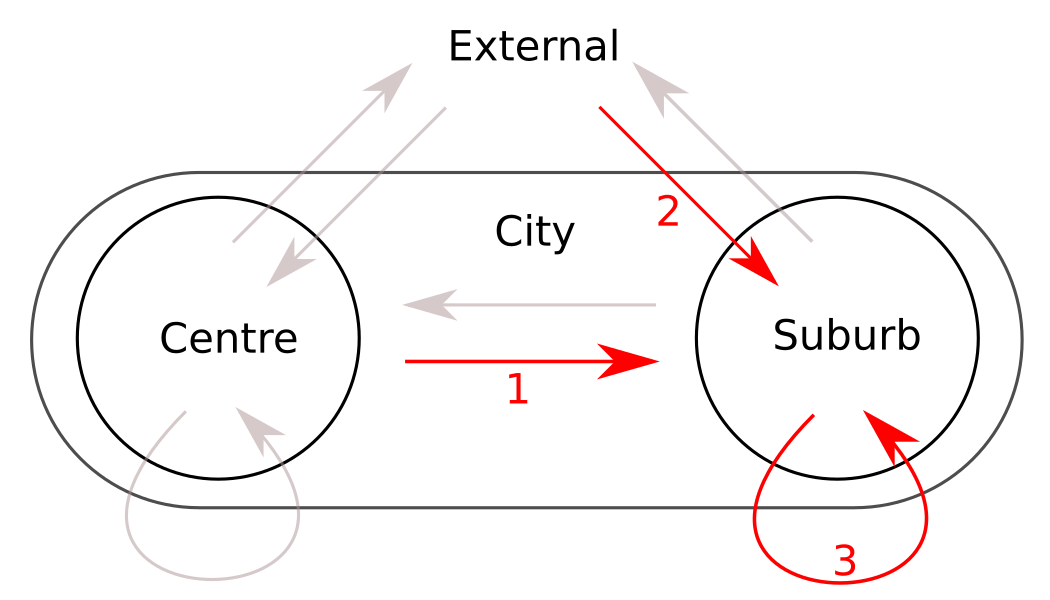
\includegraphics[width=3in]{figures/pathways.png}
		\caption{Theoretical individual geographic pathways to suburban poverty}
		\label{path}
	\end{center}
\end{figure}




\section{Data \& Methods}

Our methodology consists of several steps. First we use census and land use data to cluster neighbourhoods, specifically categorizing whether or not they are suburban (see Section 4.1). Second, we link this suburb-centre typology to an individual-level panel dataset of tax filers across Canada. Once we have this linked data, we describe overall trends of suburbanization of poverty by region (see Section 4.2). We then use this linked data to quantify the propensity of different pathways to suburban poverty described in our conceptual framework. Specifically for this analysis, we tabulate among residents in suburban poverty, the proportions of whom were living in different locations a year prior (e.g. what percent moved from a central neighbourhood, what percent immigrated in the past year, etc.), and examine how these proportions vary by CMA and how they change over time (see Section 4.3). In sum, our results provide new evidence of suburbanization of poverty in Canadian cities and how it is being formed.

Our analysis examines the nine largest Census Metropolitan Areas (CMA) in Canada. CMAs are agglomerations of municipalities where at least 50\% of the employed labour force works in the region's core \cite{statistics_canada_dictionary_2016-1}. While not perfect definitions of what consist of an urban area, CMAs are commonly used as study areas for urban research in Canada, and have been specifically used to examine neighbourhood change \cite{walks_income_2013,grant_changing_2020} and suburbanization of poverty \cite{ades_are_2012,allen_suburbanization_2021}. In descending order of their population in 2016, the nine CMAs for this study are Toronto, Montréal, Vancouver, Calgary, Edmonton, Ottawa-Gatineau, Winnipeg, Québec, and Hamilton. Each of these CMAs had a population of greater than 700,000 in 2016, while all other CMAs in Canada had a population of less than 600,000. In 2016, these nine CMAs accounted for 55\% of Canada's population.



% could do a line plot of popultion over time?

% para on their prev research of neigh change in these cities

%In  Canada,  there  is  evidence  of  increasing  income  inequalities  both  within  and  between  re-gions  (Walks,  2013;  Bolton  &  Breau,  2012;  Breau,  2015;  Chen,  Myles,  &  Picot,  2012),  as  wellas concentrations of low-income households forming in some inner-suburban neighborhoods(Ades  et  al.,  2012;  Pavlic  &  Qian,  2014;  Ades  et  al.,  2016;  Breau  et  al.,  2018).   For  example,Pavlic and Qian (2014) classified census tracts by density, age of housing stock, and distance todowntown and found that there has been decline or stagnation in prosperity in inner-suburbanareas relative to central areas and newer outer-ring suburbs. Research by Ross et al. (2004) andAdes et al. (2012) computed spatial segregation indices on low-income households and house-holds in poverty in Canadian cities, each finding that economic segregation is increasing at aneighborhood level and that low-income households are becoming increasingly concentratedand isolated within cities’ spatial units. Statistical mapping exercises have also highlighted thatneighborhoods with higher concentrations of low-income households are located further fromthe downtown core over the past several decades (Ades et al., 2012; Breau et al., 2018).


% rough description, e.g. Cg and Ed a bit newer, 

% Age of their development. Calgary and Edmonton, for example, have undergone the vast majority of their growth since World War Two, QQQ suburban compared to eastern cities. - move to results?



\subsection{Classifying Suburbs}

Our analysis begins by classifying neighbourhoods based on their urban form via a cluster analysis. The main objective of this analysis is to encode the suburban status of different neighbourhoods in order to subsequently link to data on residential mobility.

Creating classifications of neighbourhoods has a long history \cite{booth_life_1902,shevky_social_1955} and there is currently a rich literature on generating typologies of neighbourhoods via quantitative cluster analysis techniques  \cite{delmelle_differentiating_2017,silver_markov_2021}. However, most existing research has focused on clustering based on demographic and socio-economic characteristics (often framed in terms of geodemographics or market segmentation). Fewer studies have used clustering on urban form variables to try to specifically characterize whether or not a neighbourhood is suburban. Previous research that has attempted to identify suburban neighbourhoods within a city have instead adopted threshold approaches that define suburbs based on whether a neighbourhood has certain attributes above or below specific thresholds (e.g. if the population density is less than $\theta$) \cite{moos_suburban_2015,airgood-obrycki_suburban_2019}. While simple to interpret, these approaches are limited by their arbitrary selection of thresholds (e.g. the selection $\theta$). 

% Other previous research has also adopted creating numeric indices of sprawl-compactness, based on dimensionality reduction techniques like factor analysis \cite{ewing2014measuring}. However, such indices are limited in terms of discerning qualitative differences among neighbourhoods with similar scores as well as inability to assess hierarchical grouping of neighbourhoods. 

To generate classifications of Canadian suburbs, we adopt a combined hierarchical $k$-means approach. Similar approaches have been used in studies generating socio-economic typologies of neighbourhoods in Toronto \cite{silver_markov_2021} and across the United Kingdom \cite{vickers_creating_2005} to limit the drawbacks of solely using hierarchical or partitional methods (e.g. such as the random selection of cluster centres in $k$-means).
% Importantly, for our analysis, this approach allows us to initially differentiate between suburbs and central neighbourhoods (as in our conceptual framework shown in Figure \ref{path}), and it further allows us to examine different groups of suburban neighbourhoods. 
Specifically, the hierarchical $k$-means method is a three step process; it first uses hierarchical clustering to cut the tree into $k$-clusters, then it computes the means of each cluster, and third it uses $k$-means to group observations based on these cluster means. For our study, we initially aim to generate two clusters, \textit{centre} and \textit{suburb}, in order to subsequently examine pathways to poverty in the suburbs. However, our approach could be extended to generate sub-groups of each (this is noted as a direction for future work in the concluding section of this paper).

We use Census Tracts (CT) as spatial representations of neighbourhoods, because of data availability and because they are the most common spatial unit used in neighbourhood change studies in Canadian cities \cite{allen_new_2018,grant_changing_2020}. CTs usually have a population between 2,500 and 8,000 residents. Variables inputted into our cluster analysis are described below. These variables were selected based on their use in previous studies to measure how suburbanized a neighbourhood is, each capturing an important dimension of suburbanization, as well as data availability for Canadian CMAs at the CT level.

\begin{itemize}
	\item \textit{Population density.} Suburbs are often characterized as having lower densities than central neighbourhoods \cite{torrens2000measuring,hanibuchi_does_2012, massey_suburbanization_2018,airgood-obrycki_suburban_2019}. We thus use population density based on data from the 2016 Canadian census as an input into our cluster analysis.
	
	\item \textit{Age of housing}. While the history of suburbs in North America date back to before the 20th century, the sprawling scale and hyper-automobile focused design of suburbs expanded greatly after World War Two \cite{airgood-obrycki_suburban_2019,harris_creeping_2020}. Similar to previous studies measuring suburbanization \cite{hanibuchi_does_2012,ades_is_2016,airgood-obrycki_suburban_2019}, we also include a variable into our cluster analysis that pertains to age of housing, specifically the percentage of dwellings in a neighbourhood that were built after 1945.
	
	\item \textit{Type of housing}. Suburban housing is commonly characterized as being composed of single-detached dwellings 	\cite{moos_suburban_2015, ades_is_2016}. 
	% In Canadian cities, some suburban neighbourhoods also include semi-attached housing and apartment buildings. Particularly during the mid-20th century, there were a number of apartment buildings erected in the inner-suburbs. In the late 20th and early 21st centuries, there were also development of new urbanist neighbourhoods with a variety of housing types in peripheral suburban locations \cite{xu_is_2017}. 
	As such, we include a variable for the percent of dwellings in an neighbourhood that are single-detached.
	
	\item \textit{Regional accessibility}. Accessibility, within the context of urban and transportation geography, often refers to the ability to reach activity destinations in a reasonable amount of time \cite{hansen_how_1959,geurs_accessibility_2004}. (A very simple measure of regional accessibility is distance from a neighbourhood to the central business district). More detailed accessibility to jobs measures are often used as a proxy for regional accessibility, and have specifically previous been used to assess how centralized (or suburbanized) a neighbourhood is \cite{torrens2000measuring,zhang_dynamics_2020}. For our study, we make use of previously generated measures of transit accessibility to jobs that were designed to allow for comparison between regions by accounting for competition for employment and multi-modal transportation networks, including detailed transit schedules \cite{allen_measure_2020}. We use a transit accessibility measure, rather than an auto accessibility measure to additionally account for transit deficits in suburban areas. (However, it should be noted that transit accessibility and auto accessibility measures are quite correlated, with $r = 0.84$, so they would likely achieve similar results). The mathematical formulation and description of input datasets for the transit accessibility measure borrowed from \citeA{allen_measure_2020} are described in the Appendix.
	
	\item \textit{Local accessibility}. Local built environment and accessibility measures are often used to assess the effects of sprawl on health outcomes \cite{ewing_relationship_2003}, travel behaviour \cite{ewing_travel_2010}, and specifically to quantify how suburban a neighbourhood is \cite{ewing2014measuring}. For this study, we use the Proximity Measures Database (PMD) produced by Statistics Canada, which consists of walking distances to various amenities at the census dissemination block level \cite{statistics_canada_proximity_2020}. We sum the standard scores of walking access to eight types of destinations; pharmacies, childcare, healthcare, primary education, secondary education, libraries, parks, and grocery stores to create an overall metric of local amenity proximity and walkability. Details on each individual component are included in the Appendix.
	
\end{itemize}

Prior to clustering, CTs from all nine CMAs were combined into one dataset, and then all variables are normalized. This allows for direct comparison of results between cities, since all variables and results are based on the same scale. All input data were based on data circa 2016 when there were 3,947 CTs across all nine CMAs in total. However, 44 CTs were missing data in 2016, so they were not included in the cluster analysis, resulting in an $n = 3,903$. The omitted 44 CTs only accounted for 0.006\% of the overall population. 


\subsection{Measuring Suburbanization of Poverty}

Next we link this neighbourhood typology to longitudinal micro-data, specifically to the Longitudinal Administrative Database (LAD) \cite{government_of_canada_longitudinal_2020}. The LAD is a 20\% Bernoulli sample of tax filers across Canada. Sampling is completely random across Canada, so there is no non-random bias for any particular geographic area. The data consists of an annual panel, and includes a suite of information that residents note on their tax returns. In 2006, $n = 2,551,013$ in all nine CMAs combined, and in 2016, $n = 2,965,778$. The data include a vector of sampling weights, which we use for all of our analysis and presenting data as population totals. The data also denote births and are additionally linked with immigration records indicating whether, and if so when, residents immigrated into Canada. The LAD has primarily been used for research on examining usage of tax saving accounts \cite{berger_empirical_2019}, regional labour markets \cite{albouy_local_2019}, and income over the life course \cite{denton_age-income_2019}. Importantly, the LAD denote the six-digit postal code (which usually consist of a single apartment building or city block) as well as the CT of residence on December 31st for each tax year meaning they have great potential to also be used for research on residential mobility, and specifically for this paper, analyzing individual pathways to suburban poverty. Given the individual nature of the data, the data were accessed at Statistics Canada's secure Research Data Centre (RDC). Because of privacy concerns, any tabular data outputs from the RDC could only be exported as population-level weighted totals and individual cells of exported tabular data had to have a minimum of 100 unweighted observations.

The main variable of interest is the low-income status of tax filers. We use this variable as an indicator of household poverty. In the LAD, low-income status is pre-coded as a binary classification based on the Low-Income Measure (LIM). The LIM is a threshold defined by Statistics Canada whether the household has an income less than 50\% of the regional median adjusted household income---where adjusted pertains to dividing a household's income by the square root of the number of members in the household. This is to account for when a household increases in size, its needs increase, but at a decreasing rate. The LIM is provided as a before-tax and as an after-tax measure. We use the after-tax measure for our analysis. The LIM has previously been used to assess poverty in Canada among recent immigrants \cite{picot_immigration_2014}, in relation to transit accessibility \cite{allen_sizing_2019}, and analyzing food insecurity \cite{brown_money_2019}. 

For our study, linking this data to the results of the cluster analysis described in the previous section allows for describing the growth or decline of poverty in Canadian suburbs. We track this with three indices. The first is simply the total number of residents living below the poverty line in the \textit{suburbs}, $L_S$. This allows for understanding the overall scale of suburban poverty and how it has changed over time. Our next two indices are similar to the centralization indices described by \citeA{duncan_methodological_1955} and previously used in Canada with census data \cite{ades_are_2012}, but are re-focused on poverty concentration in the suburbs rather than the centre. Specifically, the second index we calculate is the percent of that population that is below the LIM threshold who live in the \textit{suburbs}, $L_S / (L_S + L_C)$, i.e. this is the probability of living in the \textit{suburbs} if living under the poverty line. However, this index is limited since it does not account for the overall population, or the growth or decline of such, in the \textit{suburbs} relative to the \textit{centre} (i.e. $L_S / (L_S + L_C)$ may be increasing mainly because the overall population in the suburbs, $N_S$, is increasing as well). As such, thirdly, we compute a relative measure to show whether poverty has suburbanized over time relative to the centre. This is the poverty rate in the \textit{suburbs} divided by the poverty rate in the \textit{centre}, $(L_S / N_S) / (L_C / N_C)$. An increase in this ratio indicates that poverty is suburbanaizing over time. This index is similar to the commonly used centralization index \cite{duncan_methodological_1955,massey_dimensions_1988}, but is based on the dichotomous results of our multivariate cluster analysis, rather than distance to the central business district.


% LAD data dictionary (2014) https://www23.statcan.gc.ca/imdb-bmdi/document/4107_D9_T15_V2-eng.pdf

% LAD more info https://crdcn.org/datasets/lad-longitudinal-administrative-databank





\subsection{Mobility Pathways to Suburban Poverty}

Importantly, this linked data allows for describing the individual geographic pathways to suburban poverty based on the conceptual framework outlined in Section 3. The data are annual panel data, meaning that individuals can be tracked over time. For our study, we are interested in whether and how residential locations changes over time, specifically in reference to those who are poor and living in the suburbs. 

We first quantify for each year, $t$, for different population groups, population counts pertaining to where they were living the year prior (i.e. in $t-1$). These counts are represented as $N_{i,j}$. For example, if $i$ is living in a city centre in year $t-1$, and $j$ is living in the suburbs in year $t$, then $N_{i,j}$ is the number of residents currently living in the suburbs ($j$) that lived in the city centre ($i$) the year prior. We have several categories of prior residential states ($i \in I$). For states 1-4, the data are further divided by low-income status.


% $P_{i|j}$ where $i$ and $j$ pertain to residential locations at time periods $t-1$ and $t$ respectively.   For our main analysis, proportions are held to $\sum_j P_{i|j} = 1$. 

\begin{enumerate}
	\item Same postal code (i.e. most likely did not move during the one-year time period).
	\item Moved from the \textit{centre} of their CMA (based on the cluster analysis results).
	\item Moved from a \textit{suburb} in their CMA (based on the cluster analysis results).
	\item Moved from elsewhere in Canada, but from outside their current CMA.
	\item Immigrated from another country.
	\item Persons born within the past year (included because the data represent entire populations)
\end{enumerate}

And we have four current residential states, $j \in J$, at time $t$, as follows. Our focus is on the transitions to low-income prevalence in the suburbs, while the other three serve as comparisons. 

\begin{enumerate}
	\item Low-income people living in a \textit{suburb}. 
	
	\item Low-income people living in the \textit{centre}
	
	\item Not low-income people living in a \textit{suburb}, 
	
	\item Not low-income people living in the \textit{centre}
\end{enumerate}

We use $N_{i,j}$ to then estimate the probability of coming from state $i$, given being in state $j$. In other words, this directly allows for showing among those in suburban poverty, the percent of which came from each of the different states, $i$. Similar statistics have been computed in residential mobility research tracking moves between different types of tenure \cite{withers_methodological_1997} and components of housing quality \cite{patel_effects_2020}. These are computed as follows:



\begin{equation}
P(i|j) = 100 \frac{N_{i,j}}{\sum_j N_{i,j}}
\end{equation}


The multiplication by 100 is to represent results as percents. We generate $P(i|j)$ and first summarize our results for the average proportions across a 10 year period (2006 to 2016). Second, we plot $P(i|j)$ for each pair of years in order to examine how these have changed over time. And third, we summarize for each CMA to highlight how different urban regions have varying propensities in their pathways to suburban poverty. 

Additionally we compute what the probability is of moving to state $j$, given previously being in state $i$. For example, this allows for showing, for different groups of people (e.g. international immigrants), what the probability is that they will end up in poverty and living in the suburbs in the following year. This is computed as follows:


\begin{equation}
P(j|i) = 100 \frac{N_{i,j}}{\sum_i N_{i,j}}
\end{equation}





\section{Results}

\subsection{Classifying Suburbs}

We first present the results of grouping neighbourhoods based on their urban form. The initial partition ($k = 2$) of our analysis classifies census tracts as \textit{suburb} and \textit{central} neighbourhoods. The means of the cluster input variables for these two groups are shown in Table \ref{table:k2}. Similar to previous research, we find that one of our groups (which we thus term as \textit{suburban}), neighbourhoods have a much lower population density \cite{hanibuchi_does_2012, massey_suburbanization_2018,airgood-obrycki_suburban_2019}, local accessibility \cite{ewing2014measuring}, and regional accessibility \cite{torrens2000measuring,zhang_dynamics_2020}, while having a much greater propensity of single-detached dwellings \cite{moos_suburban_2015, ades_is_2016}.


\begin{table}[h]
	\small
	\centering
	\caption{{Summary statistics (2016) of the partition of census tracts into two groups}}
	\label{table:k2}
	\begin{tabular}{lll}
		\hline
		& \textit{Centre}    & \textit{Suburb}   \\ \hline
		\textit{n} census tracts   & 994     & 2,909     \\
		Total population (1000s)         & 4,080   & 14,319 \\
		Mean population density (persons / km$^2$)        & 10,217   & 2,772     \\
		Mean detached dwellings         & 13.5\%   & 53.7\%    \\
		Mean post-1945 dwellings           &  75.1\%       &  97.1\%        \\
		Mean regional accessibility (Z) & 1.26    & -0.446   \\
		Mean local accessibility (Z)    & 1.23    & -0.428   \\
		\hline
	\end{tabular}
\end{table}

\begin{figure*}[h]
	\setlength{\fboxsep}{0pt}%
	\setlength{\fboxrule}{0pt}%
	\begin{center}
		\centering
		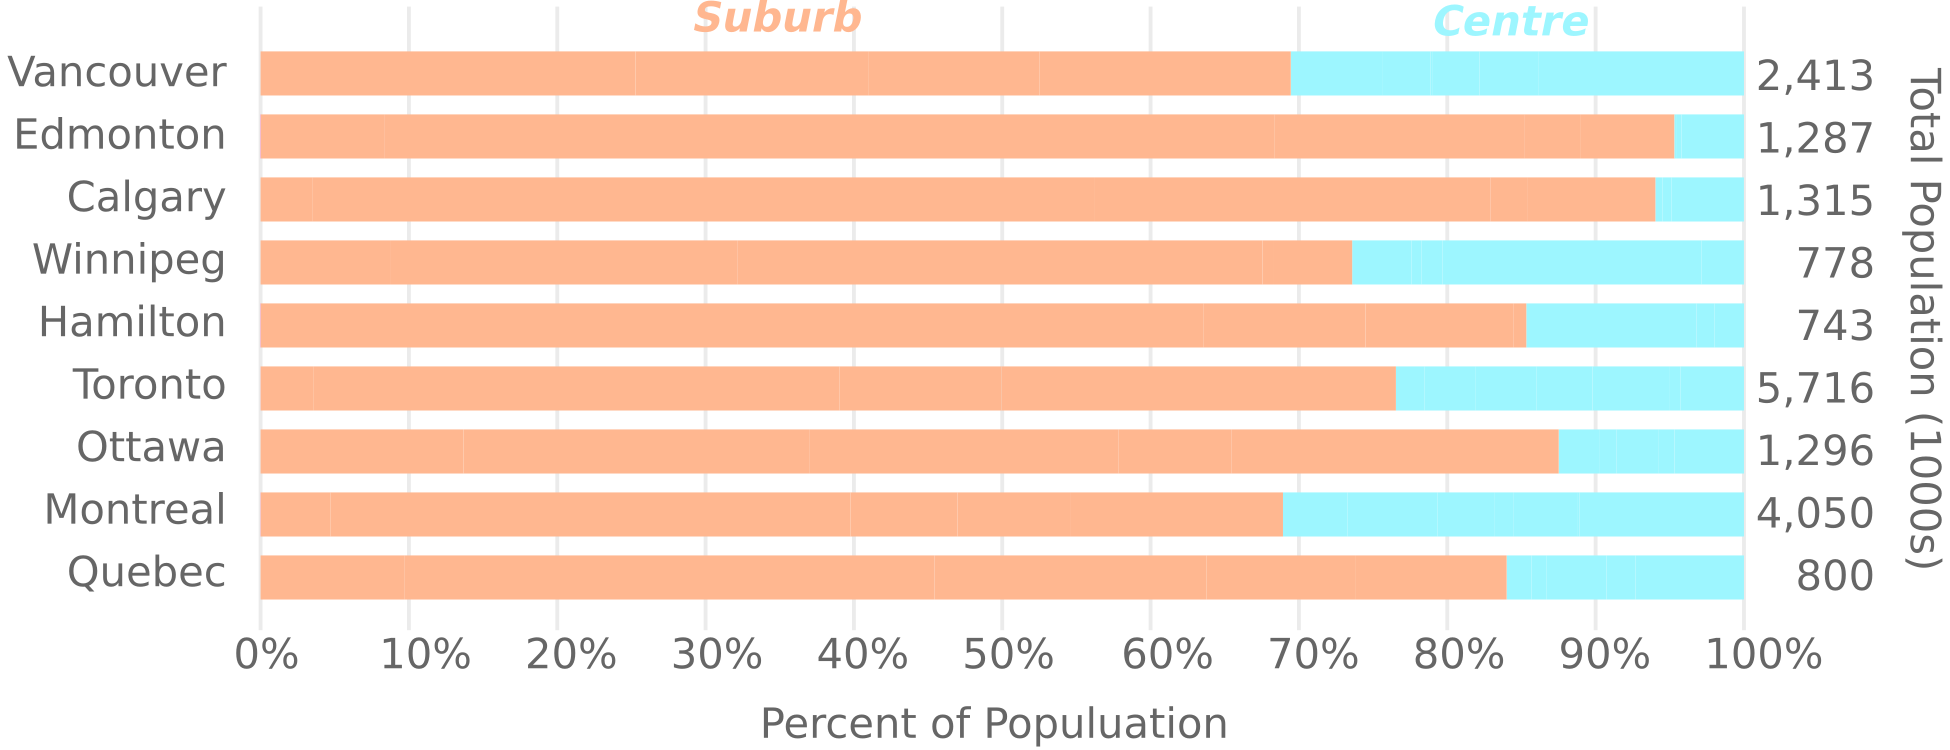
\includegraphics[width=5in]{figures/cluster_by_city.png}
	\end{center}
	\caption{Distribution of population for each cluster group by CMA}
	\label{kcma}
\end{figure*}



Census tracts from nine CMAs were inputted into the cluster analysis. However, because of the varying histories of growth and local policies as well as environmental constraints in each CMA, each has a different spatial distribution of urban form typologies, and importantly, different proportions of neighbourhoods that are classified as a \textit{suburb}. Figure \ref{kcma} displays the distribution of cluster groups in each CMA (maps of each CMA are included in the Appendix). For all CMAs, the majority of the population lives in suburban neighbourhoods. This is expected since the population of most of these CMAs has more than tripled since 1945, and the majority of urban development has been of a suburban form. Montreal and Vancouver have the lowest percent of their population living in suburban areas, with just under 70\%. In Montreal's case, this is mainly because it was the largest Canadian city during the 19th and early 20th century, and thus has the greatest extent of pre-auto-oriented development. For Vancouver, the relatively lower percent of suburbs is partly due to geographic constraints (mountains and the ocean) limiting sprawl. Conversely, in Calgary and Edmonton, approximately 95\% of the population lives in the suburbs. These two Albertan cities have few topographic constraints and the vast majority of their urban development has occurred during the auto-oriented post-war period.




% \newpage

%\begin{figure*}[h]
%	%	\setlength{\fboxsep}{0pt}%
%	%	\setlength{\fboxrule}{0pt}%
%	\begin{center}
%		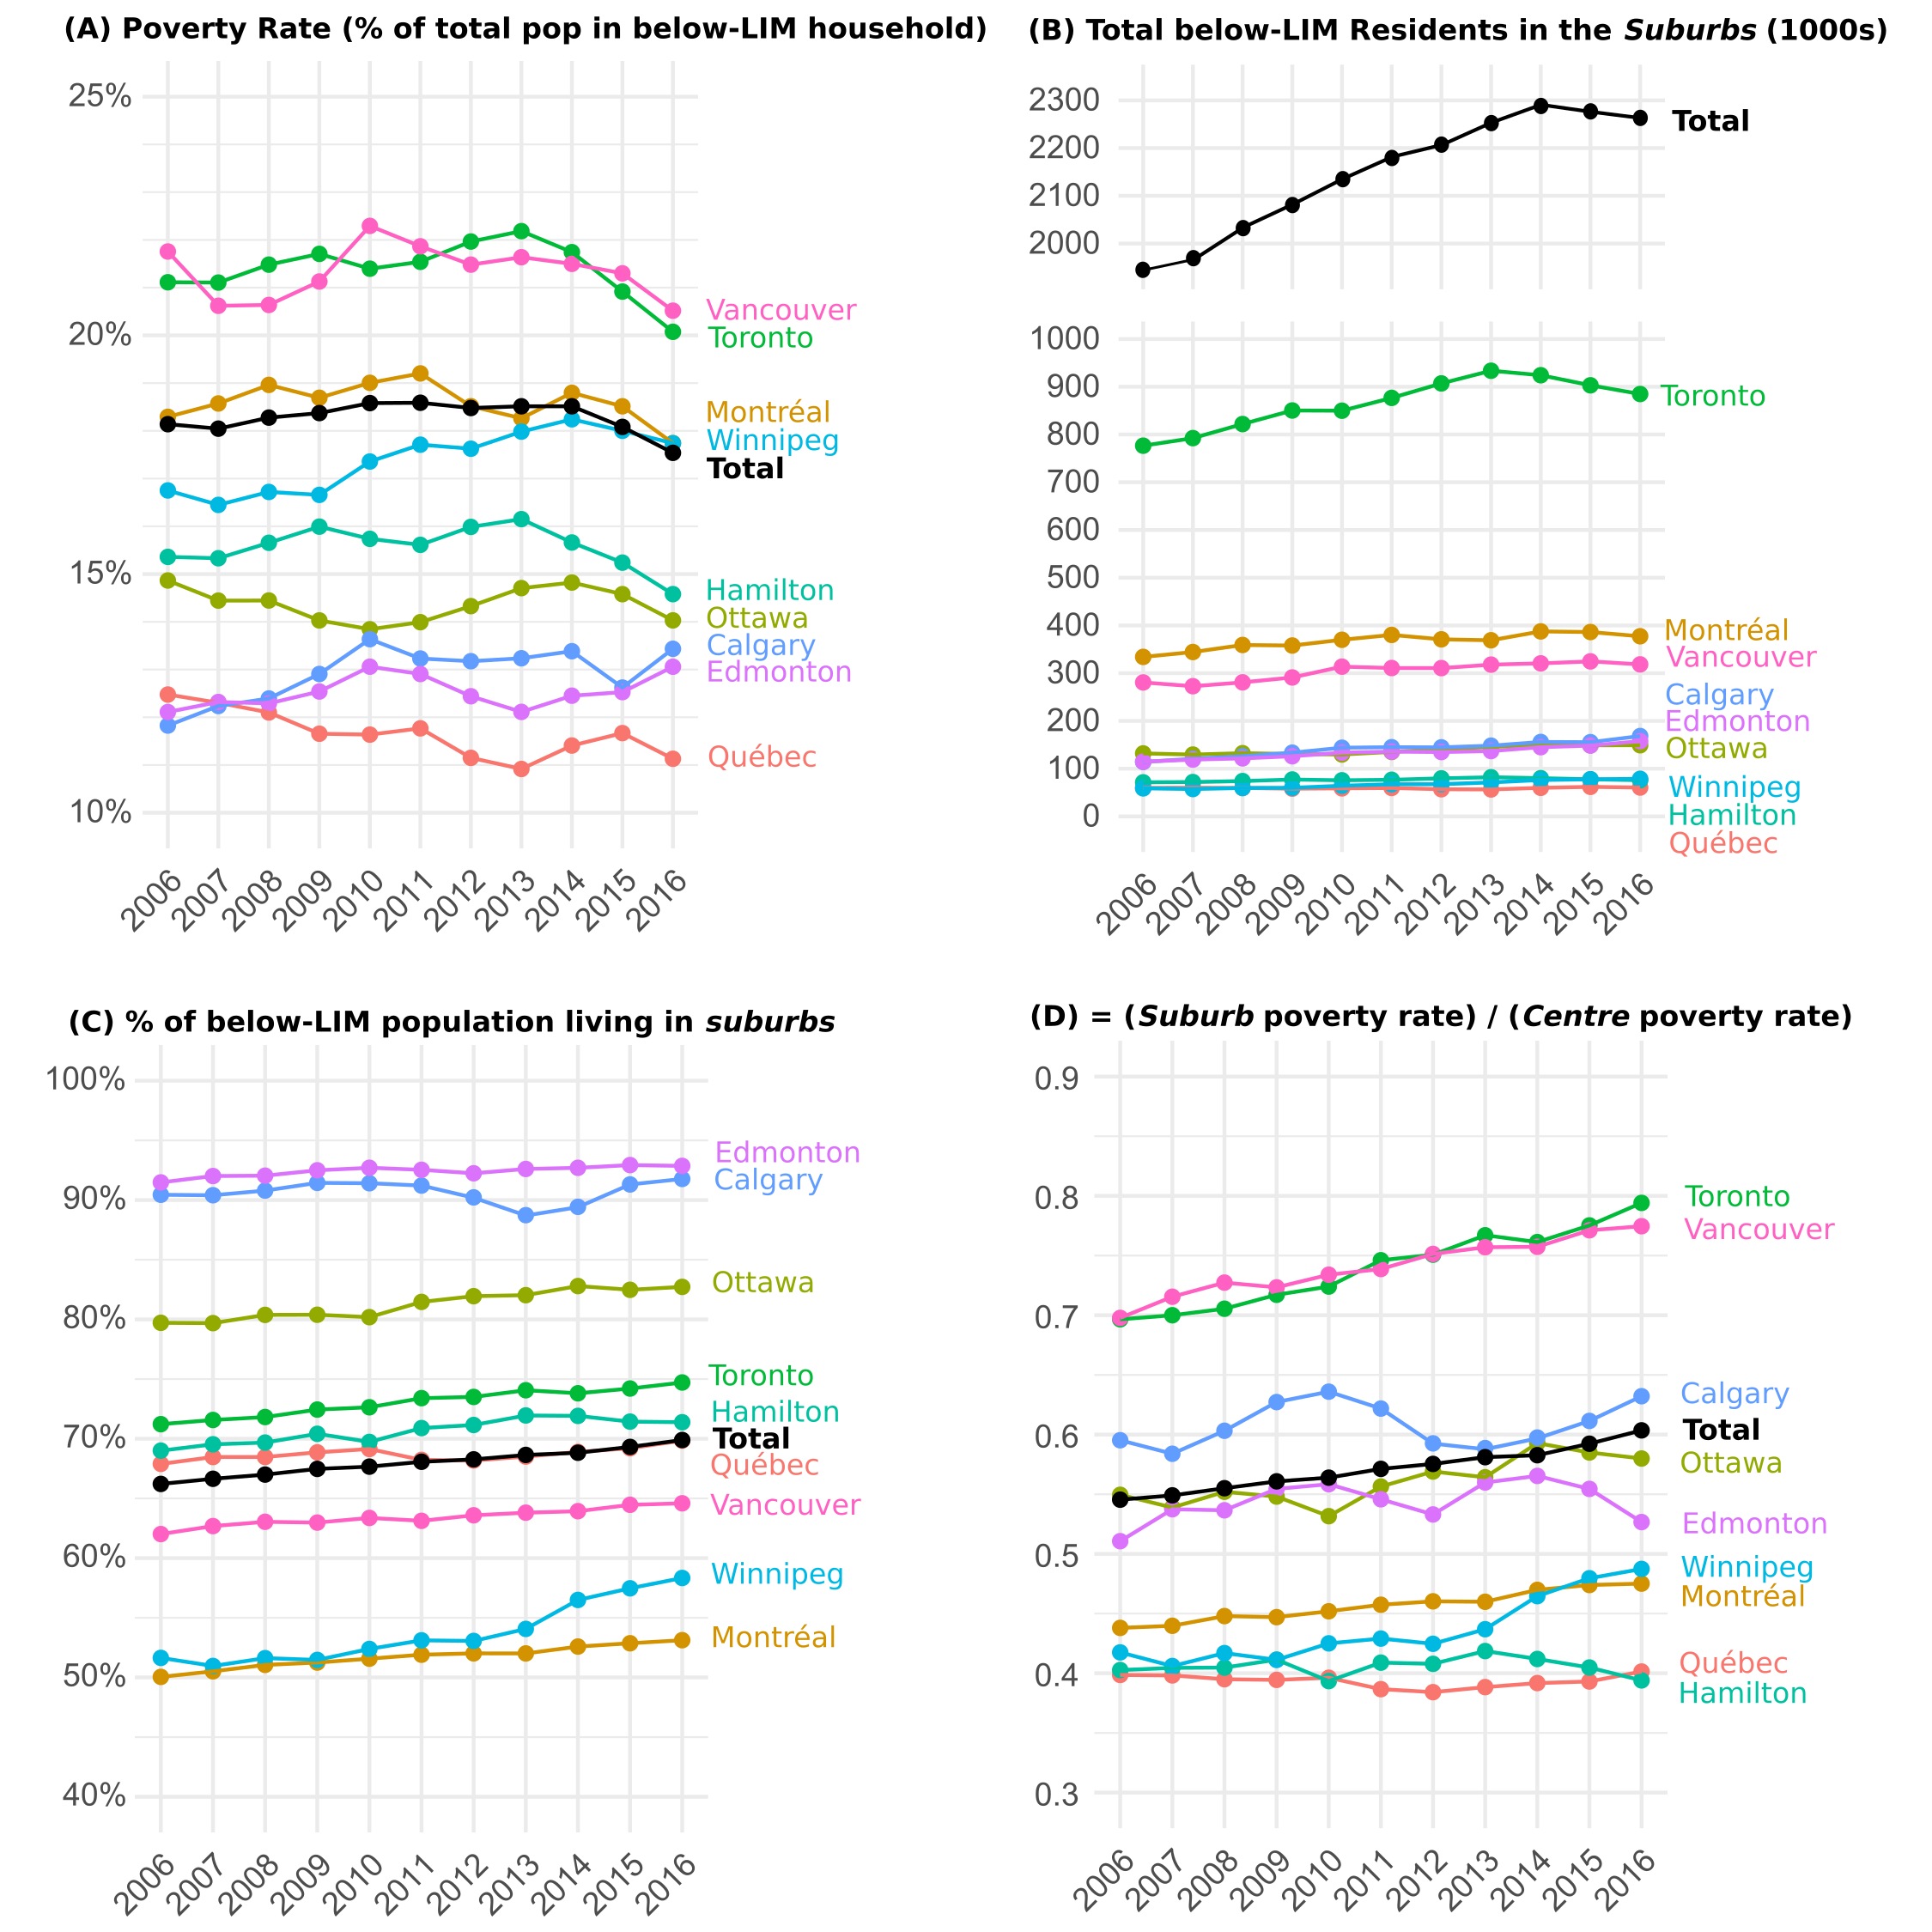
\includegraphics[width=6.5in]{figures/E_subpov4.png}
%	\end{center}
%	\caption{Plots tracking suburbanization of poverty in Canadian CMAs (2006 to 2016)}
%	\label{fig:subpov4}
%\end{figure*}





\begin{figure}[H]
	\centering
	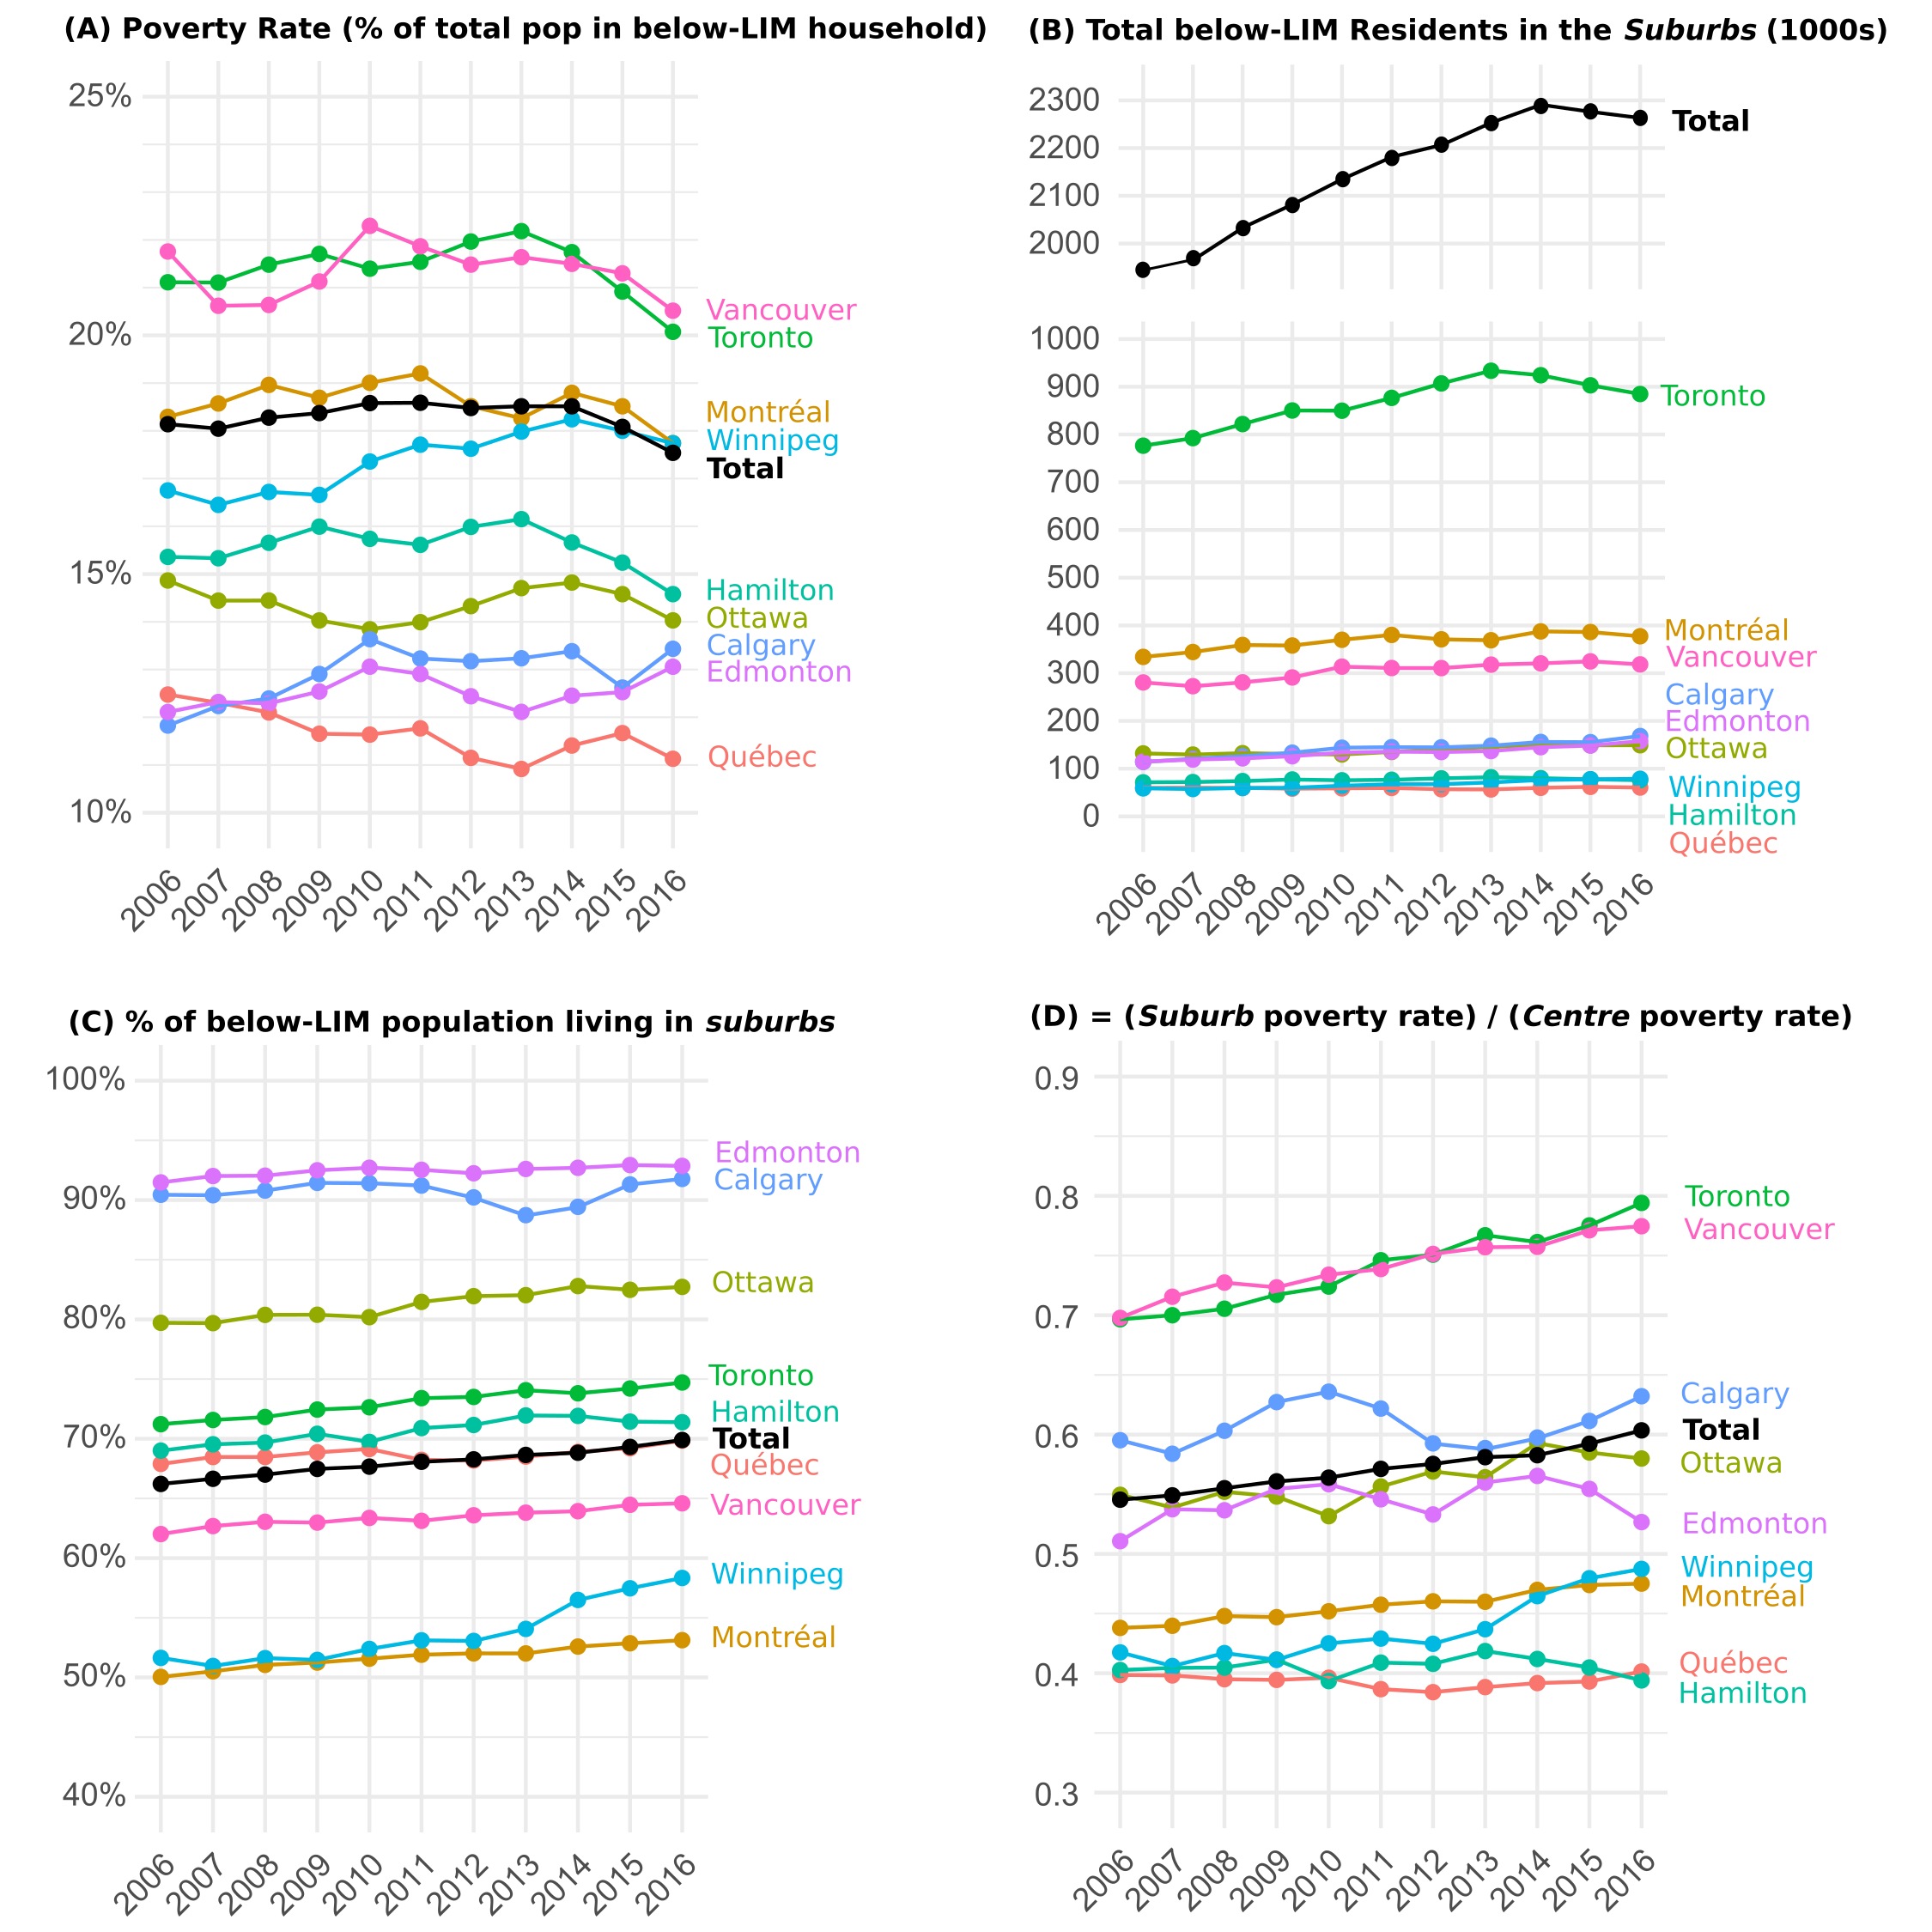
\includegraphics[width=6.5in]{figures/E_subpov4.png}
	\caption{Plots tracking suburbanization of poverty in Canadian CMAs (2006 to 2016)}
	\label{fig:subpov4}
\end{figure}


\subsection{Measuring Suburban Poverty}

In this section, we show how the prevalence suburban poverty has changed over the study period (2006 to 2016) via a series of plots (Figure \ref{fig:subpov4}). First, for context, Figure \ref{fig:subpov4} (A) shows the overall poverty rate within each CMA based on the LIM. The larger cities (Vancouver, Toronto, and Montreal) have the greatest poverty rate, and overall, the poverty rate has declined over this ten year period, in particular form 2014 to 2016. Figure \ref{fig:subpov4} (B) shows the total count of residents under the poverty line living in neighbourhoods classified as \textit{suburbs}. We see that this is increasing up until 2014, when it drops slightly in concordance with an overall drop in the poverty rate. Figure \ref{fig:subpov4} (C) plots the percent of poverty in a CMA located in the \textit{suburbs}, showing increasing trends over time. However, the overall population living in the suburbs may also be increasing over this time period. Thus in Figure \ref{fig:subpov4} (D) we plot a ratio of the poverty rate in the \textit{suburbs} to the poverty rate in the \textit{centre}. Since this ratio is less than 1 in all cases, this indicates that the poverty rate remains greater in the centre than in the suburbs. However the gap between these two poverty rates is closing. Toronto and Vancouver are the two CMAs where this gap is narrowest and closing the quickest. These plots indicate that while the overall poverty rate in Canadian cities has declined slightly from 2006 to 2016, poverty in the suburbs has increased both in absolute and relative terms.






\subsection{Mobility Pathways to Suburban Poverty}

In our conceptual framework, we outlined three aggregate mobility pathways to suburban poverty: 1) centre-to-suburb, 2) immigration, and 3) staying in the suburbs. We now examine to what the extent of these pathways occur in Canadian CMAs. These pathways are summarized as proportions in Table \ref{table:p1} with current states, $j$, dichotomized by above-LIM and below-LIM households and by \textit{suburb} and \textit{centre}. Including these four states allows for showing how mobility pathways to suburban poverty (the rightmost column) differ from other states. We find that overall, for those in suburban poverty in Canadian CMAs, 88.5\% lived in the suburbs a year prior (12.7\% moved within the suburbs, 75.8\% stayed in the same postal code), 2.9\% moved from the \textit{centre}, and 6.6\% immigrated from elsewhere (4.6\% internationally). Overall, transitioning to suburban poverty on an annual basis is more due to staying or moving within the \textit{suburbs} compared to external immigration and moving from \textit{centre} neighbourhoods. Part of this finding is due to the suburbs being home to the majority of residents (77.8\%), but this doesn't tell the whole story. Importantly, looking at the low-income suburban residents who lived in the \textit{suburbs} a year prior, 21.5\% were not categorized as low-income in the previous year, meaning that becoming poor while staying in the suburbs encompass a greater percent of suburban poverty than moving in from elsewhere. Comparatively, those in poverty in the \textit{centre}, 15.4\% had dropped into poverty during the previous year. This difference indicates that residents are more likely to drop into poverty in suburban locations than in central, more accessible, neighbourhoods. This is likely partly explaining the trends shown in Figure \ref{fig:subpov4} (D) where the poverty rate in the \textit{suburbs} is increasing more than the poverty rate in the \textit{centre}. Similar to previous research in the United States \cite{delmelle_new_2020}, Table \ref{table:p1} also shows that residents in poverty are much more likely to have moved in the past year. Particularly notable is the extent of suburb-to-suburb mobility, 12.7\% for those in suburban poverty, compared to only 7.5\% for those not in poverty. 

\begin{table*}[h]
	\small
	\centering
	\begin{center}
		
		\caption{{Mobility pathways, $P(i|j)$, to different states, $j$, averaging across from 2006 to 2016 for residents in all 9 CMAs}}
		\label{table:p1}
		\begin{tabular}{llrrrr}
			\hline
			\multicolumn{2}{l}{}                        & \multicolumn{4}{c}{Current state, $j$}                  \\
			\multicolumn{2}{c}{}          & \multicolumn{2}{c}{Above poverty line} & \multicolumn{2}{c}{Below poverty line} \\
			Prior state, $i$                  & Prior poverty status      & \textit{Centre}       & \textit{Suburb}       & \textit{Centre}      & \textit{Suburb}    \\ \hline
			{International immigrant} &  & \textbf{0.6}          & \textbf{0.3}          & \textbf{5.2}         & \textbf{4.6}       \\ \arrayrulecolor{lightgray}\hline
			Internal migrant        & No              & 1.2          & 0.9          & 0.8         & 0.7       \\
			& Yes             & 0.2          & 0.1          & 1.2         & 1.3       \\ 
			\multicolumn{2}{l}{}                        & \textbf{1.4}          & \textbf{1.0}          & \textbf{2.0}         & \textbf{2.0}      \\ \arrayrulecolor{lightgray}\hline
			Moved from \textit{centre}         & No              & 5.8          & 1.2          & 2.3         & 0.7       \\
			& Yes             & 1.0          & 0.2          & 8.1         & 2.2       \\
			\multicolumn{2}{l}{}                        & \textbf{6.8}          & \textbf{1.4}         & \textbf{10.5}       & \textbf{2.9}      \\ \arrayrulecolor{lightgray}\hline
			Moved from \textit{suburbs}        & No              & 3.4          & 6.8          & 1.7         & 4.0       \\
			& Yes             & 0.5          & 0.8          & 3.8         & 8.7       \\
			\multicolumn{2}{l}{}                        & \textbf{3.9}          & \textbf{7.5}          & \textbf{5.4}         & \textbf{12.7}      \\ \arrayrulecolor{lightgray}\hline
			Stayed in same               & No              & 80.3         & 85.0         & 13.1        & 17.5      \\ 
			postal code & Yes             & 5.8          & 3.5          & 62.3        & 58.3      \\
			\multicolumn{2}{l}{}                        & \textbf{86.1}         & \textbf{88.5}         & \textbf{75.3}        & \textbf{75.8}      \\ \arrayrulecolor{lightgray}\hline
			\multicolumn{2}{l}{Births}                  &\textbf{ 1.2}         & \textbf{1.3}          & \textbf{1.6}         & \textbf{1.9}      \\ \arrayrulecolor{black}\hline
			\multicolumn{2}{l}{Total}                   & 100.0        & 100.0        & 100.0       & 100.0   \\ \arrayrulecolor{black}\hline
		\end{tabular}
	\end{center}
\end{table*}






\begin{figure}[H]
	\centering
	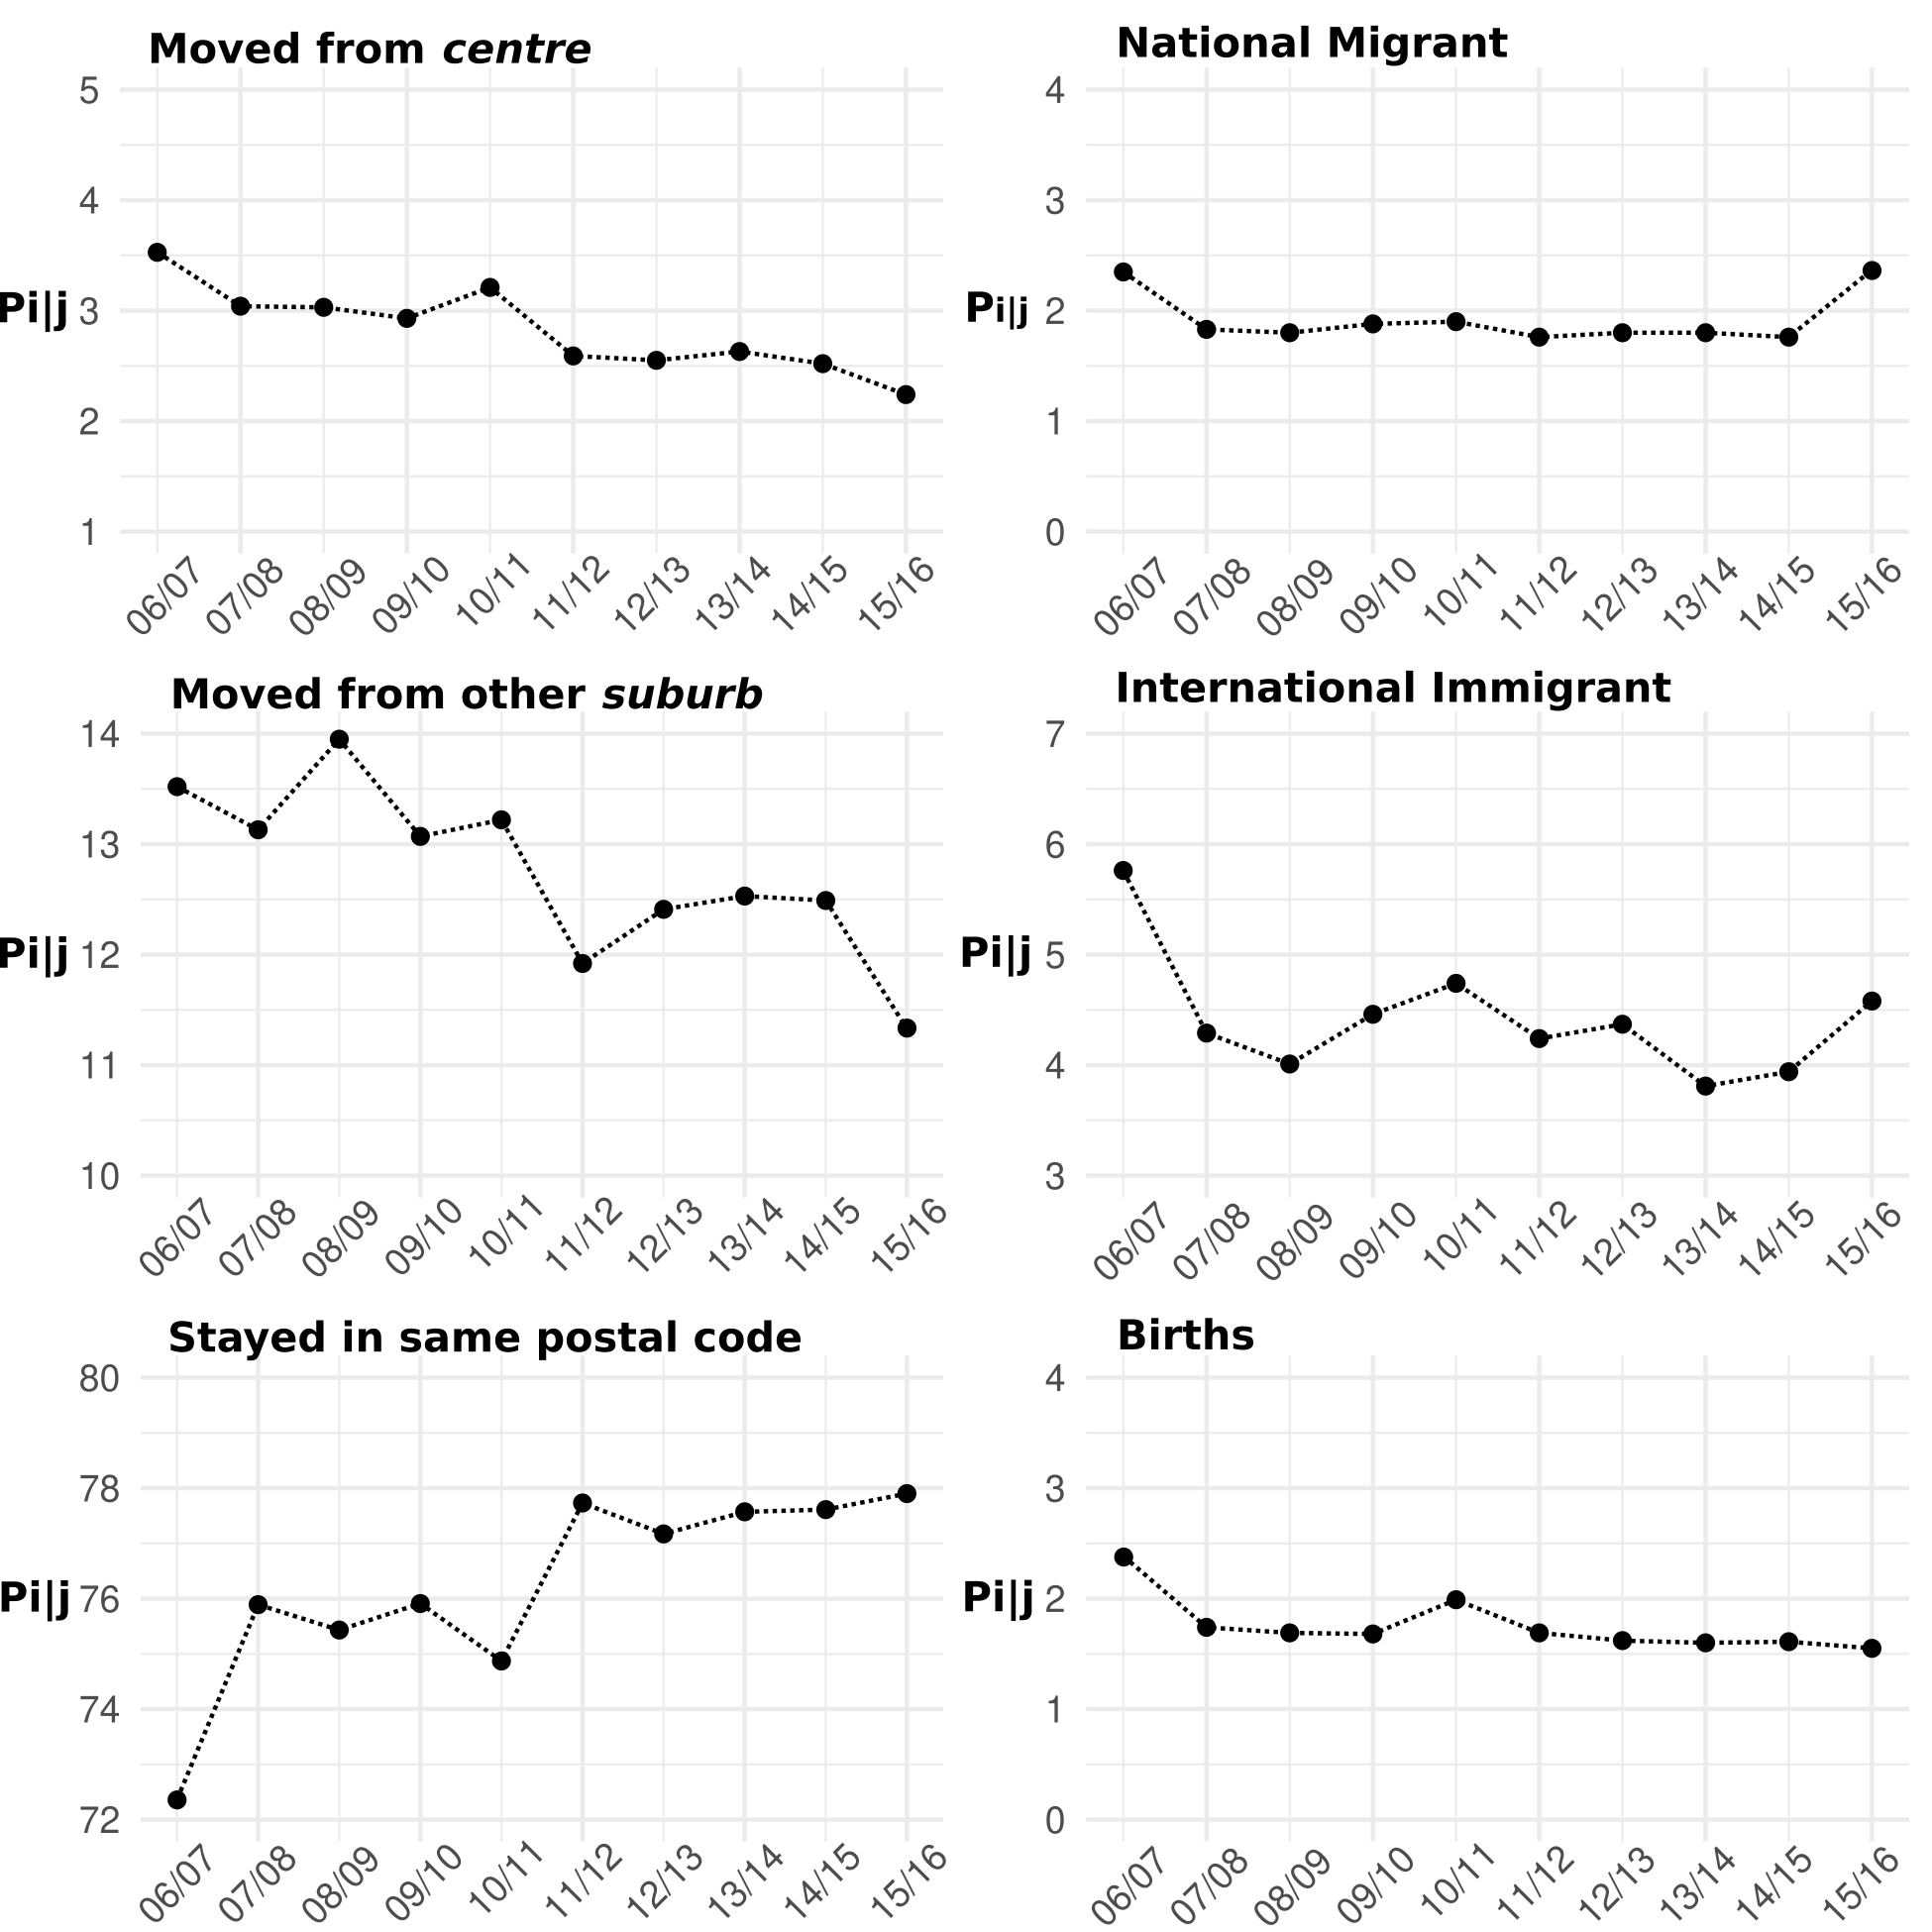
\includegraphics[width=4.9in]{figures/transitions_by_year.png}
	\caption{Mobility pathways, $P(i|j)$, to suburban poverty by year}
	\label{fig:tbyr}
\end{figure}


Figure \ref{fig:tbyr} shows how yearly transitions to suburban poverty have changed from 2006 to 2016. Overall, there has been a decline in the percentage of people in suburban poverty who moved from a different location within the region a year prior, both in terms of moving from another \textit{suburb} and moving from the \textit{centre}. This is offset by the proportion for not moving increasing over this time period. The percent of low-income immigrants from elsewhere in Canada and new births have remained relatively stable over time, while the proportion of international immigrants is a bit more sporadic.



We then turn our attention to differences in mobility transitions to suburban poverty by CMA (see Table \ref{table:pcma}). While the trends are relatively similar across all regions, there are some notable differences. The prairie cities of Edmonton, Calgary, and Winnipeg, show that not moving has lower proportions than the rest of Canada, while immigration, particularly international immigrants, account for a greater proportion of poverty in the suburbs in these cities. \textit{Suburb}-to-\textit{suburb} mobility is also greater in Edmonton and Calgary, mainly because the suburbs account for a relatively greater extent of the region than other cities (e.g. see Figure \ref{kcma}).  \textit{Centre}-to-\textit{suburb} residential mobility is greatest in Winnipeg, Vancouver, and Montreal indicating that gentrification-induced displacement may be greater in these three CMAs than in others. International immigration accounts for a greater proportion in Vancouver and Toronto than in other eastern cities. These two cities have high immigration rates over the study period, and have been described as having growing ethnic enclaves in suburban areas \cite{grant_changing_2020}. Of all nine CMAs, Hamilton has the greatest proportion of suburban poverty stemming from residents immigrating from elsewhere in Canada.






\begin{table}[h]
	\small
	\centering
	\caption{{Mobility pathways, $P(i|j)$, to suburban poverty by CMA (averaged from 2006 to 2016)}}
	\label{table:pcma}
	
	\makebox[\textwidth][c]{
		\begin{tabular}{ll p{1.2cm}p{1.2cm}p{0.9cm}p{1.1cm}p{1.1cm}p{1.0cm}p{0.9cm}p{1.0cm}p{1.0cm}}
			\hline
			&  &
			\multicolumn{9}{c}{CMA}                                                                                                                       \\
			Prior state, $i$                & Prior LIM & Vancouver     & Edmonton      & Calgary       & Winnipeg      & Hamilton      & Toronto       & Ottawa        & Montreal      & Quebec        \\ \hline
			International migrant &            & \textbf{4.6}  & \textbf{5.3}  & \textbf{6.5}  & \textbf{8.5}  & \textbf{2.6}  & \textbf{4.7}  & \textbf{3.4}  & \textbf{2.9}  & \textbf{2.5}  \\ \arrayrulecolor{lightgray}\hline
			Internal immigrant      & No         & 0.6           & 1.4           & 1.5           & 0.6           & 1.6           & 0.4           & 1.0           & 0.4           & 1.0           \\
			& Yes        & 1.2           & 2.7           & 2.6           & 1.0           & 3.0           & 1.0           & 1.9           & 0.7           & 1.5           \\
			\multicolumn{2}{l}{}                 & \textbf{1.8}  & \textbf{4.1}  & \textbf{4.1}  & \textbf{1.6}  & \textbf{4.6}  & \textbf{1.4}  & \textbf{2.9}  & \textbf{1.1}  & \textbf{2.5}  \\ \arrayrulecolor{lightgray}\hline
			Moved from \textit{centre}       & No         & 0.8           & 0.4           & 0.4           & 1.2           & 0.6           & 0.6           & 0.5           & 0.9           & 0.8           \\
			& Yes        & 2.5           & 0.9           & 0.8           & 3.8           & 1.9           & 1.8           & 1.8           & 3.0           & 2.2           \\
			\multicolumn{2}{l}{}                 & \textbf{3.3}  & \textbf{1.3}  & \textbf{1.2}  & \textbf{4.9}  & \textbf{2.6}  & \textbf{2.4}  & \textbf{2.3}  & \textbf{3.9}  & \textbf{2.9}  \\ \arrayrulecolor{lightgray}\hline
			Moved from \textit{suburbs}      & No         & 3.7           & 6.4           & 5.8           & 3.4           & 3.5           & 3.3           & 4.2           & 4.1           & 5.0           \\
			& Yes        & 8.7           & 10.6          & 9.5           & 7.5           & 6.9           & 8.6           & 9.3           & 7.8           & 7.3           \\
			\multicolumn{2}{l}{}                 & \textbf{12.4} & \textbf{17.0} & \textbf{15.3} & \textbf{10.9} & \textbf{10.4} & \textbf{11.9} & \textbf{13.5} & \textbf{11.9} & \textbf{12.2} \\ \arrayrulecolor{lightgray}\hline
			Stayed in same            & No         & 17.4          & 21.3          & 22.4          & 17.1          & 18.2          & 16.4          & 16.3          & 17.3          & 17.3          \\
			postal code & Yes        & 59.2          & 48.4          & 48.2          & 54.6          & 59.9          & 61.7          & 59.8          & 61.5          & 61.6          \\
			\multicolumn{2}{l}{}                 & \textbf{76.6} & \textbf{69.7} & \textbf{70.6} & \textbf{71.7} & \textbf{78.1} & \textbf{78.1} & \textbf{76.1} & \textbf{78.8} & \textbf{78.9} \\ \arrayrulecolor{lightgray}\hline
			\multicolumn{2}{l}{Births}           & \textbf{1.3}  & \textbf{2.6}  & \textbf{2.3}  & \textbf{2.4}  & \textbf{1.8}  & \textbf{1.6}  & \textbf{1.9}  & \textbf{1.4}  & \textbf{1.0}  \\ \arrayrulecolor{black}\hline
			\multicolumn{2}{l}{Total}            & 100.0         & 100.0         & 100.0         & 100.0         & 100.0         & 100.0         & 100.0         &  100.0         & 100.0 \\ \arrayrulecolor{black}\hline       
		\end{tabular}
	}
	
\end{table}



\vspace{5mm}

Lastly, we present probabilities of transitioning to states $j$ (such as suburban poverty), for different prior states $i$. This is presented in Table \ref{table:pji}. Noticeable from this table is that international immigrants, as well as internal migrants who were previously in poverty, have high propensities of moving to the suburbs and remaining under the poverty line. For international immigrants, this could partly be due to not having a full year of income (and thus being more likely to be classified as below the poverty line). Immigrating to the \textit{centre} also remains relatively high. We also find that those in poverty in the suburbs have a 24.9\% chance of moving out of poverty while staying in the suburbs. Included in Table \ref{table:pji} is the population size of $N_i$, averaged over the ten year period. Multiplying this by the percents can give is overall flows (the full flow matrix is also provided in the Appendix). This allows for showing the total flows in and out of suburban poverty. On average from 2006 to 2016, 471,000 residents living in the suburbs dropped into poverty per year, while 502,000 escaped poverty. While in the \textit{centre}, 157,000 dropped into poverty per year while staying in the \textit{centre}, while 181,000 escaped poverty. The relative difference in these ratios indicates that that poverty alleviation in-place is greater in the \textit{centre} than the \textit{suburbs} 



\begin{table}[h]
	\small
	\centering
	\caption{Propensities among different groups, $i$, of moving into suburban poverty}
	\label{table:pji}
	\begin{tabular}{llrrrrr}
		\hline 
		\multicolumn{2}{c}{}                        & \multicolumn{4}{c}{Current state, \textit{j}}   &               \\
		\multicolumn{2}{l}{Prior state, \textit{i}}          & \multicolumn{2}{c}{Non-LIM} & \multicolumn{2}{c}{LIM}  & \\ 
		Location                  & LIM status      & \textit{Centre}       & \textit{Suburb}       & \textit{Centre}      & \textit{Suburb}  & $\bar{N}_i$  \\ \hline
		International immigrant & & 8.1\%        & 15.7\%       & 26.4\%      & 49.8\%  &  196,626 \\ 
		\arrayrulecolor{lightgray}\hline
		Internal migrant        & No              & 20.9\%       & 64.6\%       & 5.0\%       & 9.5\% &  151,588   \\
		& Yes             & 7.8\%        & 22.1\%       & 21.1\%      & 49.0\%  &  58,251 \\
		\arrayrulecolor{lightgray}\hline
		\textit{Centre}                    & No              & 88.2\%       & 5.2\%        & 6.0\%       & 0.6\%  &  2,599,460  \\
		& Yes             & 18.8\%       & 2.0\%        & 74.3\%      & 4.8\%  & 961,042   \\
		\arrayrulecolor{lightgray}\hline
		\textit{Suburb}                    & No              & 0.8\%        & 94.8\%       & 0.2\%       & 4.2\%  & 11,213,758   \\
		& Yes             & 0.7\%        & 24.9\%       & 1.9\%       & 72.5\%   & 2,013,613 \\
		\arrayrulecolor{lightgray}\hline
		\multicolumn{2}{l}{Births}                  & 13.4\%       & 62.8\%       & 6.8\%       & 17.0\% & 229,551   \\ \arrayrulecolor{black}\hline
		Overall Totals            &                 & 15.3\%       & 66.4\%       & 5.8\%       & 12.5\%  & 17,423,889 \\ \hline
	\end{tabular}
\end{table}



\section{Conclusions}

Suburban poverty is an increasing phenomenon in Canadian cities. This is evident in our analysis of tax records (see Figure \ref{fig:subpov4}) as well as previous research using census and other survey data \cite{ades_are_2012,breau_pulling_2018,grant_changing_2020,allen_suburbanization_2021}.

In our research, we further set out to uncover the main residential mobility transitions to suburban poverty. We find that overall, transitioning to suburban poverty on an annual basis is much more a result from staying or becoming poor within the suburbs compared to immigration or due to moving (and potentially being displaced from) gentrifying neighbourhoods in the centre. On a year-by-year basis, of the low-income suburban residents who lived in the suburbs, 21.5\% dropped into poverty while staying in the suburbs on average, compared to only 2.9\% who moved from a central area or the 6.6\% who immigrated from elsewhere. We find that these trends are similar when comparing between regions and over our study period (2006 to 2016). Despite this finding, much of the discussion in Canada on suburbanization of poverty has been directly attributed to gentrification and displacement from less affordable central neighbourhoods \cite{grant_changing_2020}. This points to further consideration into the causes of dropping into poverty in the suburbs including (but not limited to), increasing rents in suburban apartments \cite{august_gentrification_2018}, automobile debt limiting spending in other areas \cite{walks_driving_2018}, or low transit accessibility impacting ability to travel to employment, education, or social services needed for poverty reduction \cite{allen_planning_2020} 

% Specifically, for those in suburban poverty in Canadian CMAs, 88.5\% lived in the suburbs a year prior (of which, 12.7\% moved residences within the suburbs and 75.8\% did not move), 2.9\% moved from a central neighbourhood, and 6.6\% immigrated from elsewhere (4.6\% internationally, 2.0\% from within in Canada). Moreover, of the low-income suburban residents who lived in the suburbs a year prior, 21.5\% were not classified as being in a low-income in the previous year. Thus becoming poor while staying in the suburbs encompasses a greater proportion of suburban poverty than immigration and \textit{centre}-to-\textit{suburb} mobility combined. 

Our results also provide pertinent information to aid preventative policy aimed at reducing suburban poverty in Canada. For one, knowledge that a substantial portion suburban poverty stems from becoming poor in-place should expedite support for urban planning and policy to make suburbs more livable and accessible. In other words, policy for reducing suburban poverty should not parochially be focused on other pathways, such as limiting gentrification and displacement. While important to quell such displacement, our findings indicate that it is also imperative to make improvements to the suburbs, such as expanding community and social resources in the suburbs alongside more compact urban design, active travel infrastructure, and improved public transit in order to provide residents the ability to access amenities and opportunities (e.g. employment, education), as these would all be worthwhile strategies aimed at poverty alleviation in the suburbs. Our findings additionally show that international immigrants have a high propensity of settling in the suburbs and being below the poverty line. This points to policy aimed at providing incentives for more housing (e.g. as vouchers) for recent immigrants, particularly in more central locations. Overall, however, since our research was primarily descriptive and exploratory, future research should be designed to study the effectiveness of different strategies of reducing the propensity of dropping into poverty in the suburbs.

This is the first paper that we are aware of that develops a conceptual framework and empirically examines residential mobility pathways to suburban poverty. But given the exploratory nature of our analysis as well as use of a large-sample dataset, we had to make a few simplifications. As such, expanding upon these would also be important directions for future research. First, we used a single binary measure of low-income status (LIM) to classify whether a resident was in poverty in a given year. We used the LIM because it was pre-defined by Statistics Canada as well as used in other research projects \cite{picot_immigration_2014,allen_sizing_2019,brown_money_2019}. However, sensitivity analysis of results for different poverty measures, including those with multiple categories, would allow for more nuanced findings. Similarly, we generated a binary measure via a cluster analysis to describe whether or not a neighbourhood is suburban. This could be expanded to looking at multiple categories of urban form, in particular, specific types of suburban neighbourhoods. The $k$-means hierarchical clustering method we used could certainly be expanded to account for this. As well, other clustering methods could be tested to examine how and to what extent they would affect results.

Our analysis focused on year-to-year transitions from 2006 to 2016. So another important direction for future work would be to analyze individual pathways to suburban poverty prior to 2006 as well as analyze individuals over the course of multiple years. The latter could be conducted via sequence analysis methods to examine whether there are common life-course and residential mobility trajectories to suburban poverty. This could also be used to connect to longer-term neighborhood-level changes (e.g. to ask whether neighbourhoods with more concentrated poverty have a larger share of low-income people who dropped into poverty or who moved from elsewhere?). However, one drawback of using this tax record data is that it lacks contextual factors about why people move. Such factors are difficult to directly infer from tax records. Another direction for future work could be to link this data to possible push or pull factors that may disproportionately affect residential mobility of low-income residents. For example research analyzing out-mobility due to gentrification and new transit infrastructure has been conducted in the United States \cite{freeman_displacement_2005,delmelle_new_2020}, but not in Canada, and nowhere that we are aware of with the sample size of the LAD (20\% of the population). Continuing research in these directions would provide further knowledge regarding the individual pathways and neighbourhood dynamics that lead to suburbanization of poverty.






\section*{4.A \hspace{1mm} Appendix}
\addcontentsline{toc}{section}{4.A \hspace{1mm} Appendix}

\subsection*{4.A.1 \hspace{2mm} Measuring Transit Accessibility to Jobs}
\addcontentsline{toc}{subsection}{4.A.1 \hspace{2mm} Measuring Transit Accessibility to Jobs}


Transit accessibility measures were borrowed from the work by \citeA{allen_measure_2020}. These were calculated as follows.

\begin{equation}
A_{i,\lambda} = \frac{\bar A^o}{\bar A^c} \sum_{j = 1}^{J} \frac{ O_j f(t_{i,j,\lambda})}{L_{j}}
\end{equation}

$A_i$ is the accessibility measure from a zone $i$ for a transport mode $\lambda$. Where $O_j$ is the number of jobs at a zone $j$. $t_{i,j,\lambda}$ is the travel time from zone $i$ to $j$ by travel mode $\lambda$. $f(t_{i,j,\lambda})$ is a decay function weighting nearby locations more than those further away, computed as $f(t_{i,j,\lambda}) = e^{-0.023 t_{i,j,\lambda}}$. $L_j$ is a measure of access to the labour force from zone $j$. This accounts how in some regions places, there may be more jobs in proximity, but there may also be more people competing for those jobs (i.e. each job can only be filled by one worker). $L_j$ is computed as follows.

\begin{equation}
L_j = \sum_{\forall \lambda \in \Lambda} \sum_{i = 1}^{I} \frac{ \alpha_{i,\lambda} P_i f(t_{i,j,\lambda})}{A_{i,\lambda}}
\end{equation}



Where $P_i$ is the size of the labour force in zone $i$ and $\alpha_{i,\lambda}$ is the mode share for travel to work trips for mode, $\lambda$. $\Lambda$ is the overall set of travel modes, and the total mode share in each zone sums to 1, i.e. the above equation is subject to $\sum_{\forall \lambda \in \Lambda} { \alpha_{i,\lambda} = 1}$.

Since $L_j$ and $A_{i,\lambda}$ are dependent on each other, they were estimated iteratively. The fractional term in (1), $\frac{\bar A^o}{\bar A^c}$, standardizes after each iteration due to aggregate differences in the size of the labour force and total jobs in each region due to varying unemployment rates. $\bar A^o$ is the mean accessibility after the first iteration, and $\bar A^c$ is the mean accessibility after each iteration $c$.

Travel times, $t_{i,j,\lambda}$ were computed using OpenTripPlanner, incorporating walking networks from OpenStreetMap and GTFS data for transit schedules. Accessibility measures were computed for every minute during a morning commute period (7am to 9am), and then averaged, to account for fluctuating transit schedules. Population and employment data were based on the 2016 Canadian census. 


\subsection*{4.A.2 \hspace{2mm} Measuring Local Accessibility}
\addcontentsline{toc}{subsection}{4.A.2 \hspace{2mm} Measuring Local Accessibility}

Local accessibility measures were derived from the Proximity Measures Database (PMD) developed by \citeA{statistics_canada_proximity_2020}. Specifically, we generate an overall index based on proximity measures for the eight destinations noted in Table \ref{table:pmd} released at the dissemination block level. Each indicator in the PMB is released on a scale from 0 to 1, where a 0 is when there are no destinations within the network distance noted in Table \ref{table:pmd}, and a 1 is the highest value across all of Canada. All eight indicators were summed and then scaled into a standardized score prior to inputting into the cluster analysis.

\begin{table}[h]
	\small
	\centering
	\caption{{Destination types and network distances used to measure local accessibility}}
	\label{table:pmd}
	\begin{tabular}{lll}
		\hline
		\textbf{Destination}    & \textbf{Network Distance}   \\ \hline
		Grocery stores & 1km \\
		Health care & 3km \\
		Pharmacies & 1km \\
		Child care & 1.5km \\
		Primary education & 1.5km \\
		Secondary education & 1.5km \\
		Neighbourhood parks & 1km \\
		Libraries & 1.5km \\ 
		\hline
	\end{tabular}
\end{table}

\newpage



\subsection*{4.A.3 \hspace{2mm} Cluster Analysis Maps}
\addcontentsline{toc}{subsection}{4.A.3 \hspace{2mm} Cluster Analysis Maps}

Figures \ref{fig:mm1} and \ref{fig:mm2} show the spatial distribution of cluster analysis results for each CMA.


\begin{figure}[H]
	\centering
	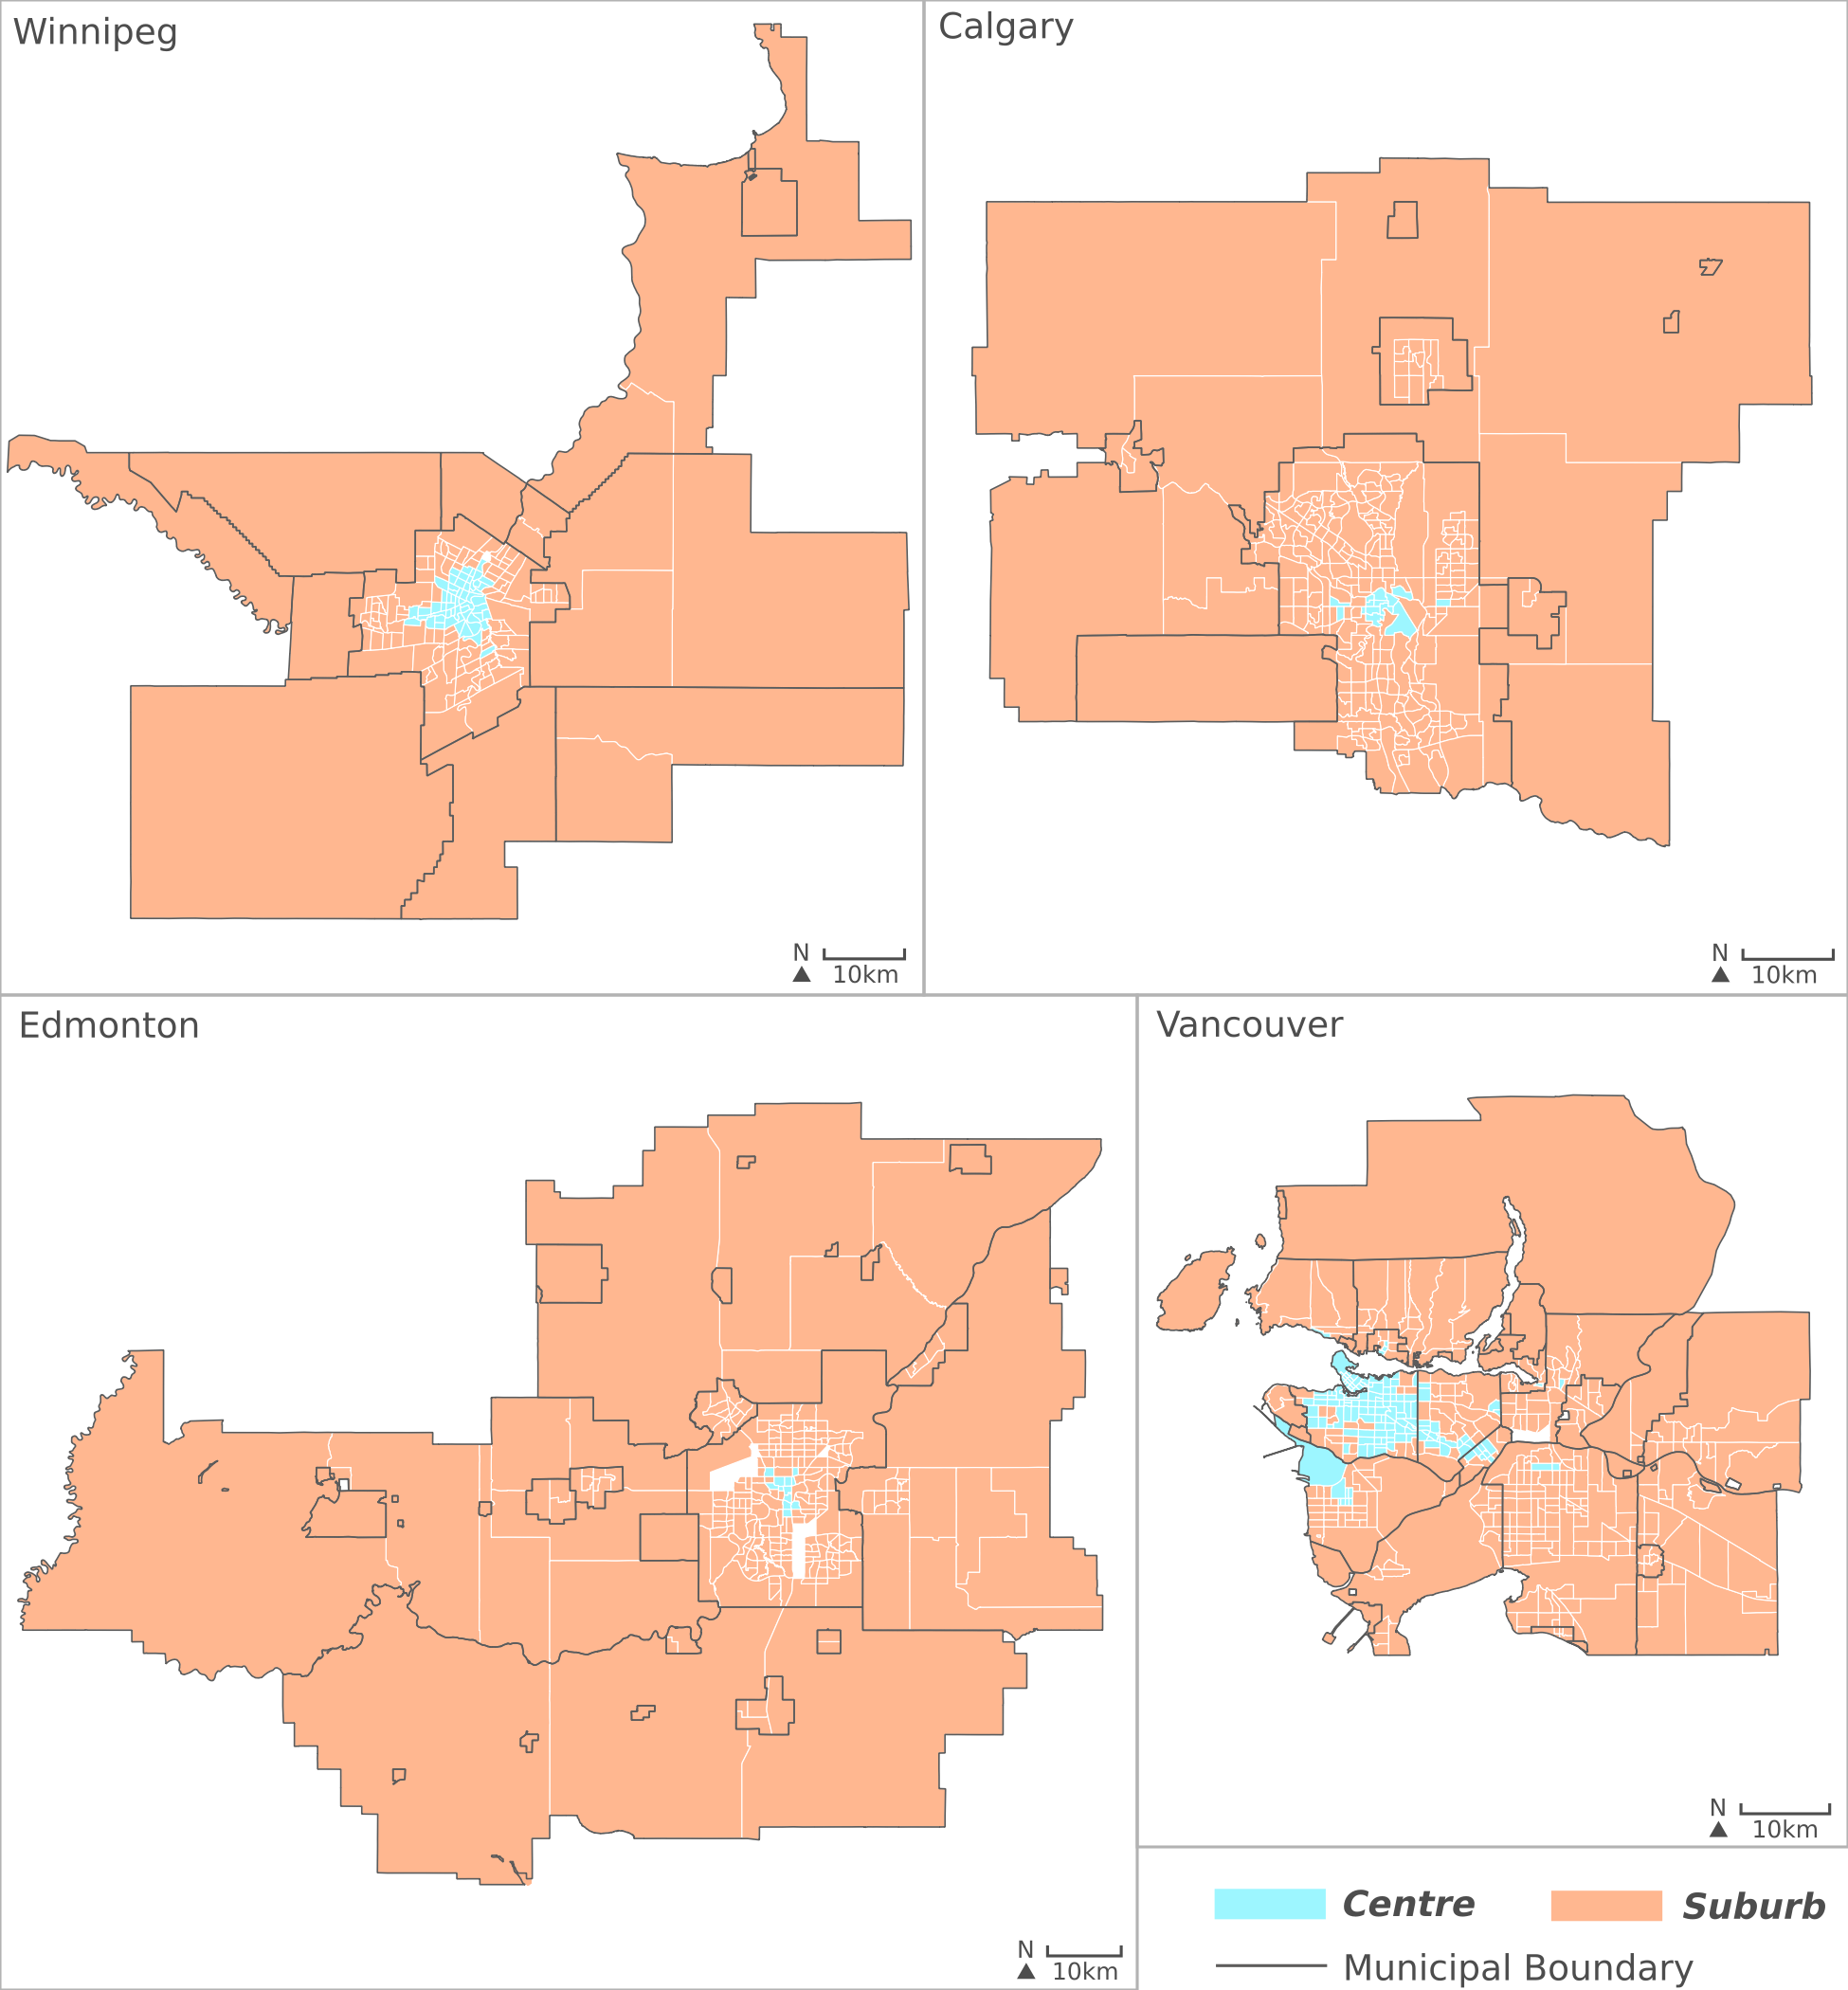
\includegraphics[width=6in]{figures/E_mini_2.png}
	\caption{Locations of \textit{centre} and \textit{subrub} clusters}
	\label{fig:mm1}
\end{figure}




\begin{figure}[H]
	\centering
	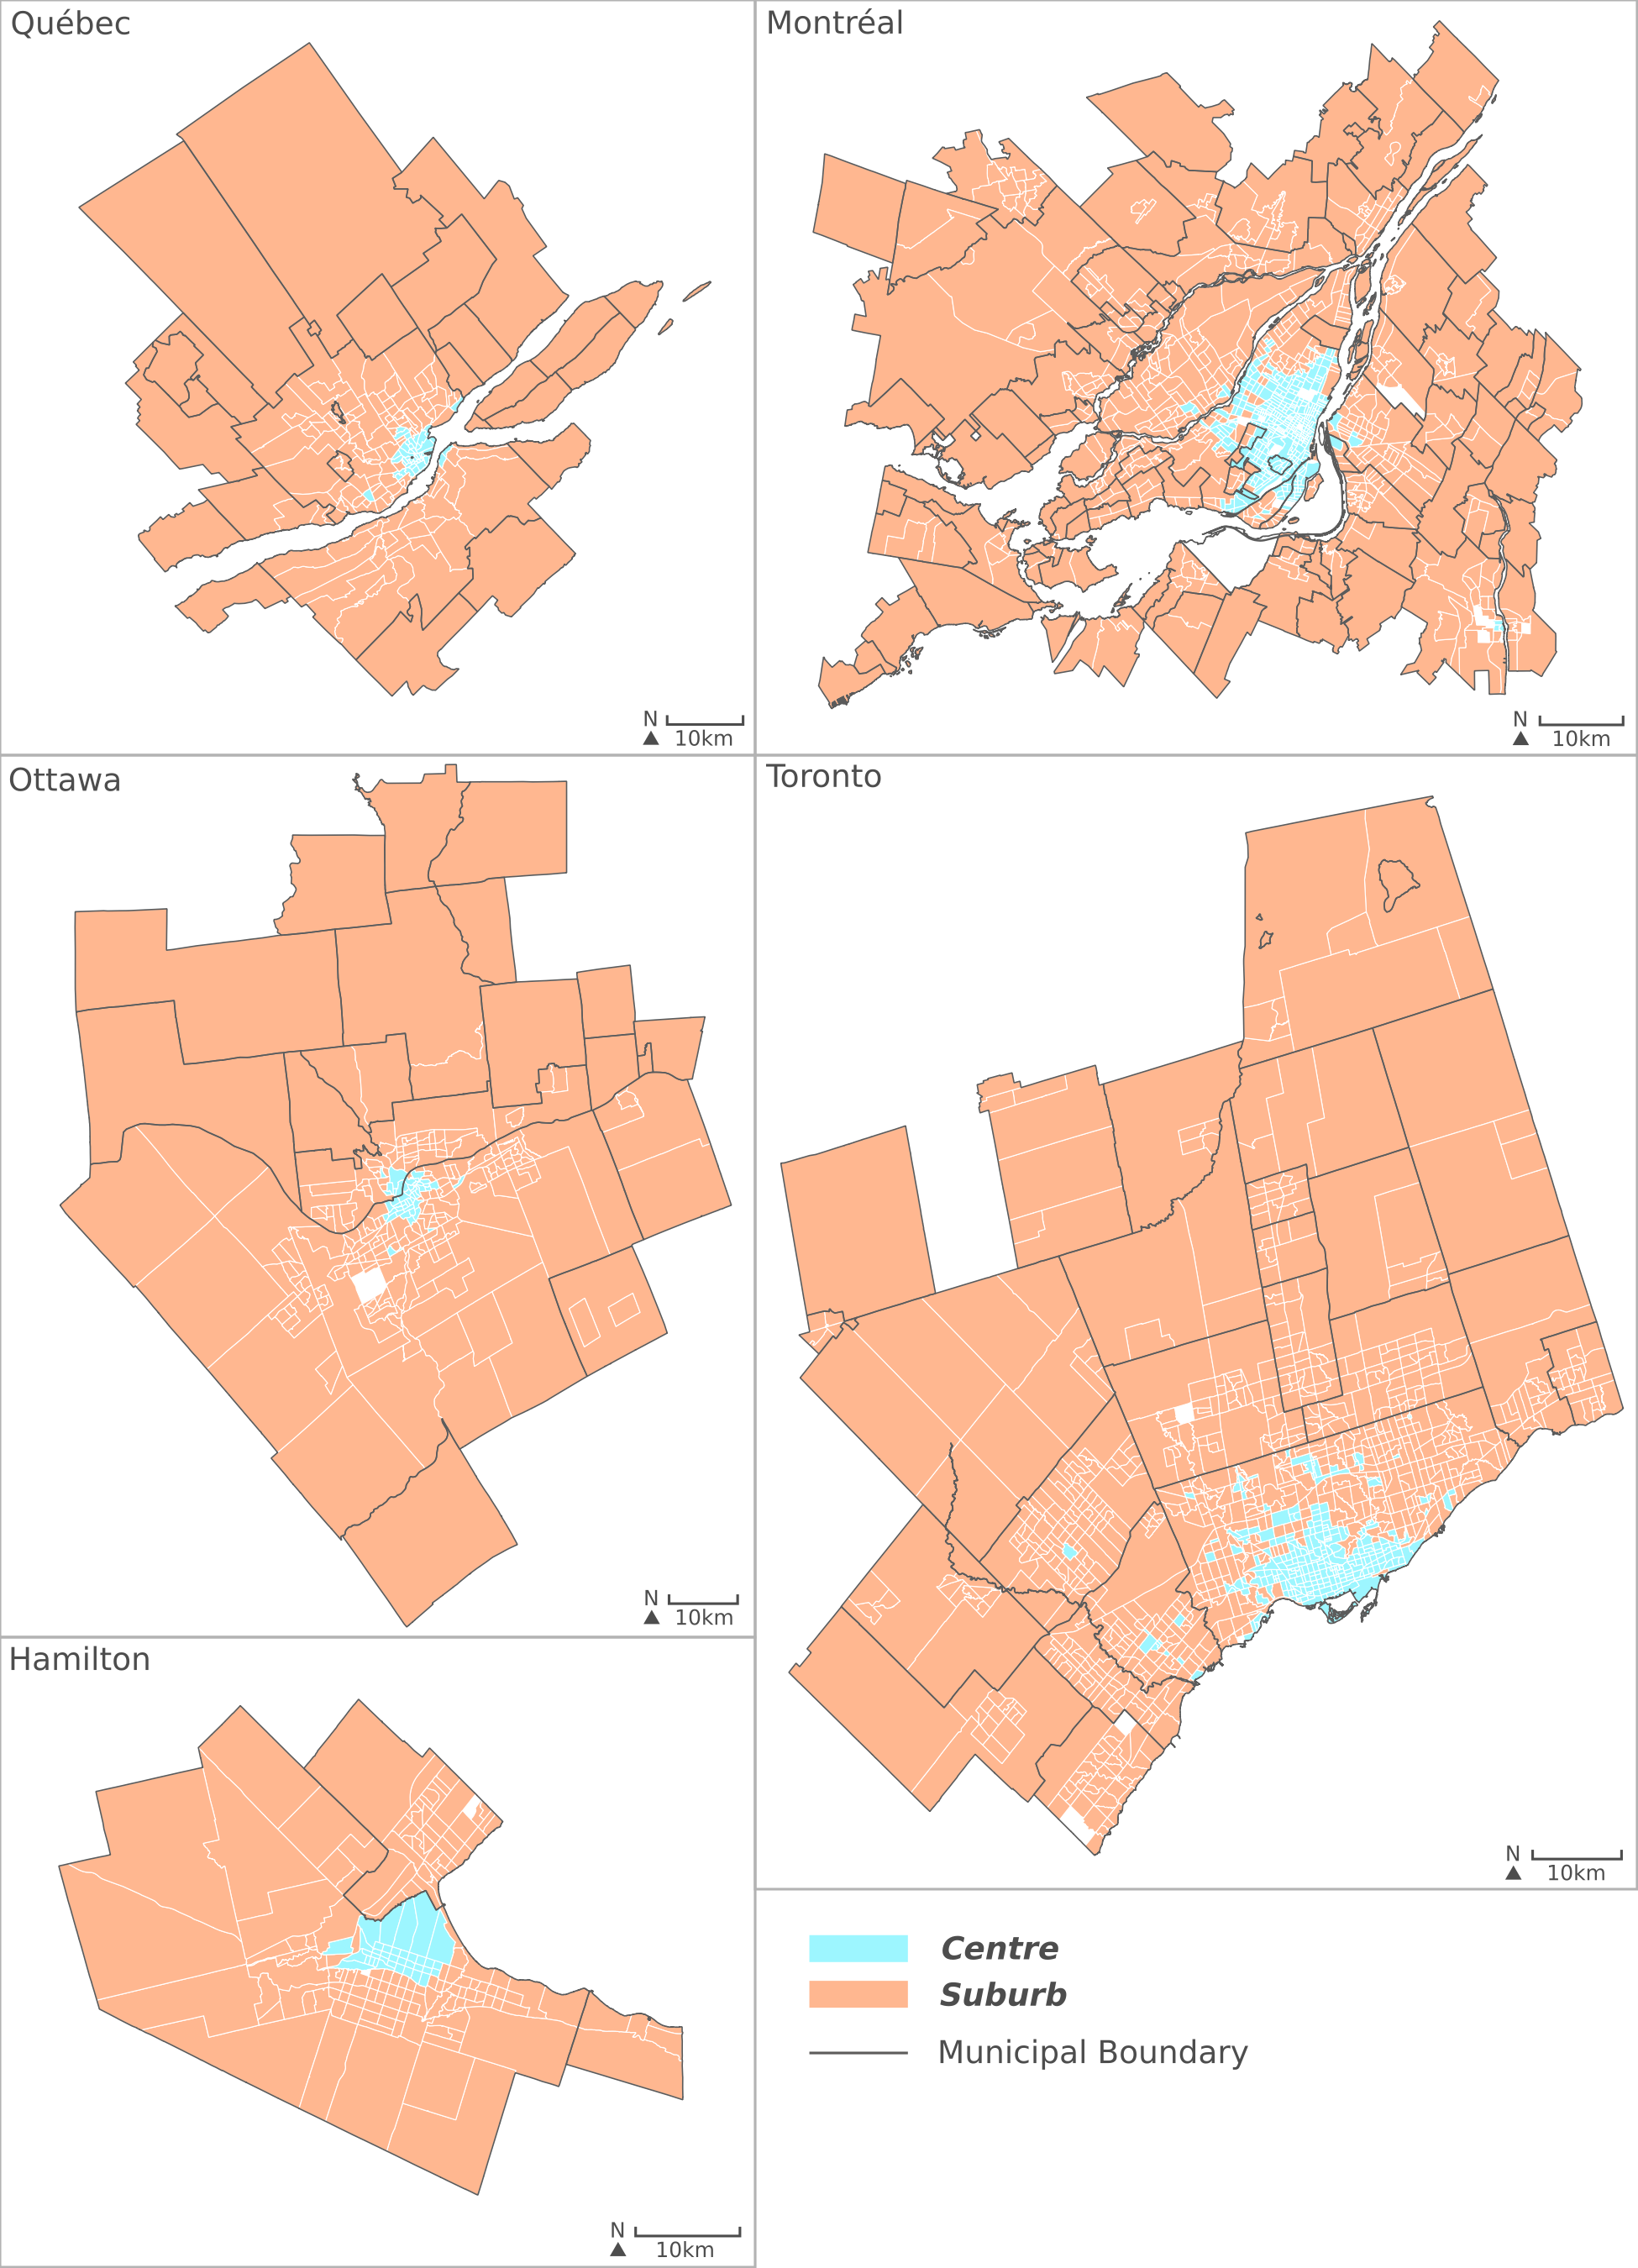
\includegraphics[width=6in]{figures/E_mini_1.png}
	\caption{Locations of \textit{centre} and \textit{subrub} clusters}
	\label{fig:mm2}
\end{figure}





\subsection*{4.A.4 \hspace{2mm} Population Flow Matrices}
\addcontentsline{toc}{subsection}{4.A.4 \hspace{2mm} Population Flow Matrices}




Table \ref{table:nij} displays average yearly population flows between different states $i$ and $j$. These values were used to generate the probabilities presented in Tables \ref{table:p1} and \ref{table:pji}.



\begin{table}[h]
	\small
	\centering
	\caption{Average yearly population flows, $\bar{N}_{i,j}$ between different states $i$ and $j$}
	\label{table:nij}
	\begin{tabular}{llrrrrr}
		\hline 
		\multicolumn{2}{c}{}                        & \multicolumn{4}{c}{Current state, \textit{j}}   &               \\
		\multicolumn{2}{l}{Prior state, \textit{i}}          & \multicolumn{2}{c}{Non-LIM} & \multicolumn{2}{c}{LIM}  & \\ 
		Location                  & LIM status      & \textit{Centre}       & \textit{Suburb}       & \textit{Centre}      & \textit{Suburb}  & Totals ($\bar{N}_i$)  \\ \hline
		
		
		International immigrant &  & 15,919    & 30,871     & 51,979    & 97,857    & 196,626    \\
		Internal migrant           & No           & 31,694    & 97,946     & 7,587     & 14,361    & 151,588    \\
		Internal migrant           & Yes          & 4,548     & 12,849     & 12,303    & 28,551    & 58,251     \\
		Centre                       & No           & 2,292,992 & 134,348    & 156,647   & 15,473    & 2,599,460  \\
		Centre                       & Yes          & 180,973   & 19,085     & 714,380   & 46,604    & 961,042    \\
		Suburb                       & No           & 91,585    & 10,633,223 & 16,914    & 472,036   & 11,213,758 \\
		Suburb                       & Yes          & 13,227    & 501,882    & 37,947    & 1,460,557 & 2,013,613  \\
		\multicolumn{2}{l}{Births}                  & 30,873    & 144,104    & 15,616    & 38,958    & 229,551    \\
		Totals ($\bar{N}_j$)                      &              & 2,661,811 & 11,574,308 & 1,013,373 & 2,174,397 & 17,423,889 \\ \hline
	\end{tabular}
\end{table}



\chapter{Are low-income residents disproportionately moving away from transit?}
\label{ch:lowinctra}
\section*{{Abstract:}}


	Lower residents are often reliant on public transit for daily travel. They have also historically concentrated in centrally located neighbourhoods with relatively higher levels of transit accessibility. However, during the late 20th and early 21st century, many urban regions have undergone trends of inner-city gentrification and suburbanization of poverty, raising concerns that low-income residents are disproportionately moving away from relied upon transit service. In this paper, we investigate what occurs when low-income residents change dwellings within a region: do they experience a reduction in their levels of transit accessibility, how does this compare to higher-income movers, and how has this changed over time? We examine this by linking historical transit accessibility measures to annual individual-level panel data representing 20\% of tax filers in Toronto, Canada from 1988 to 2018. We then analyze changes in transit accessibility for intra-urban movers via descriptive statistics and regression models to answer whether there are significant differences in individual changes in transit accessibility by low-income status. We find that low-income residents do, on average, experience reductions in their levels of transit accessibility when moving within the region, but they do not undergo as great of a reduction in transit accessibility as higher-income movers. However, the gap in experienced changes in transit accessibility between high- and low-income movers is converging over time.


\section*{{Keywords:}}

transit accessibility, residential mobility, income, displacement, exclusion



\section{Introduction}

Public transit is immensely important among lower-income urban residents for daily travel \cite{sanchez_transit_2004,giuliano_low_2005,kramer_unaffordable_2018,barri_can_2021}. In most cities, transit accessibility is greater near the centre than in more peripheral neighbourhoods. While lower-income residents tend to live in areas of greater transit accessibility on average \cite{deboosere_evaluating_2018,allen_sizing_2019}, some North American cities have undergone trends of inner-city gentrification and suburbanization of poverty over the past several decades \cite{kneebone_suburbanization_2010,ehrenhalt_great_2012,ades_are_2012, grant_changing_2020}. This means that in some places, lower-income households are increasingly living in areas with relatively lower levels of transit accessibility and thus have greater barriers to daily travel and are facing increased risks of transport-related social exclusion \cite{allen_suburbanization_2021,liu_suburbanization_2021}. 

There are also growing concerns that some transit rich neighbourhoods are becoming unaffordable and are resulting in the residential displacement and exclusion of low-income residents; but quantitative studies have mixed or inconclusive results about whether low-income residents move disproportionately out of gentrifying neighbourhoods or whether newly built transit lines directly leads to the displacement of low-income residents \cite{rayle_investigating_2015, zuk_gentrification_2018,padeiro_transit-oriented_2019,delmelle_transit-induced_2021}. However, existing research that studies income inequalities of residential mobility in relation to public transit focuses on the outcomes of specific transit routes, which serve only a fraction of the population in a region, rather than comprehensively examining changes across an entire region. As such, there is needed research to assess whether there are social inequalities at a regional level pertaining to whether lower-income residents are unequally reducing their levels of transit accessibility when they move. 

The objective of our paper is thus to answer the following: do low-income residents, on average, experience a reduction of their level of transit accessibility when they move within a region? If so, to what extent? And if so, do low-income movers witness a greater reduction in transit accessibility than higher-income movers? Specifically, we examine differences in transit accessibility resulting from intra-urban moves using an administrative dataset representing 20\% of tax-filers across an entire region (Toronto) over a 30-year period (1988 to 2018). Findings of this study are important for understanding whether there is evidence of a disproportionate number of low-income residents moving away from much relied upon public transit service, and if so, how this has changed over time. Furthermore, findings about differences in individual residential mobility patterns by income and relative to transit accessibility can offer further explanations about how contemporary trends of urban socio-spatial restructuring, such as inner-city gentrification and suburbanization of poverty, unfold within a region over time. While our empirical analysis is focused on a single region, the types of data and methods described in our paper could be applied to other regions.







\section{Background}

Many North American cities, throughout much their histories, have been characterized with income profiles of increasing wealth from the inner-city (typically where there is adequate transit service) outwards towards the suburbs (where cars are often a necessity for daily travel). Early 20th century urban sociologists described residents as moving up the social hierarchy by moving out away from the city via processes of succession and filtering, while more central neighbourhoods were places for in-migration and the working class \cite{burgess_growth_1925}. Monocentric urban conceptualizations have also been used in urban land-use theory \cite{alonso_location_1964} to explain why lower-income residents have concentrated centrally; that while households and firms make trade-offs between commuting/travel costs and housing size, the elasticity for living space for households is greater than that for travel costs, leading to central-peripheral income gradients \cite{becker_theory_1965,glaeser_why_2008}. 

The historical concentration of low-income residents in central parts of cities rather than the suburbs has also been theorized in terms of both preferences and constraints. Concentration of poverty within central areas is associated with living in a neighbourhood in which the population is overwhelmingly socially disadvantaged (e.g. crime, urban decay, pollution) as well as inaccessibility to sufficient social and community resources such as education and employment \cite{wilson_truly_2012, lucas_transport_2012,sampson_great_2012}. Such conditions can also act as push-factors persuading out-moving of residents who can afford to do so \cite{jones_neighbourhood_2021}. Land-use and transport planning can also be factors in the residential location of low-income residents in more centrally located neighbourhoods, specifically clustering in areas with greater transit accessibility. For instance, usually under sustainability objectives, regions often try to plan higher density housing (e.g. apartments) to be co-located near major transit nodes and corridors (often termed as transit-oriented development). Overall, apartments tend to have better transit connections and are also more likely to be home to low-income residents than lower-density residential dwellings. Lower-income residents also tend to have greater preferences to live near transit because of the high costs of private vehicles \cite{glaeser_why_2008}. For similar reasons, immigrants with lower incomes, on average, often tend to settle in central areas rather than in the suburbs. Immigrants also often face delays in acquiring drivers licenses, further causing reliance on and preferences for public transit \cite{blumenberg_getting_2010,blumenberg_planning_2010,lo_relationship_2011}. 

Individual decisions to move are often conceptualized as a more complex combination of household preferences at different stages-of-life as well as built environment factors, both in terms of push factors away from a neighbourhood and pull factors into desired neighbourhoods \cite{short_residential_1978,lee_residential_2010,coulter_what_2015,saghapour_role_2019}. Components of suburban living that have been considered as desirable pull factors for some households include (but are not limited to) improved access to green space, car-based lifestyles, desire for increased privacy, proximity to quality schools, perceived safety, wanting to own a home, and increased living space (larger homes and yards) that are often attractive for families with children \cite{liao_compact_2015,willing_is_2017}. Moving to the suburbs can also be due to wanting to move closer to employment \cite{huang_tracking_2018}, broader patterns of social homophily and self-selection \cite{sampson_neighborhood_2008,van_gent_sociocultural_2019}, or neighbourhood familiarity \cite{chen_decomposing_2011}. Because of the higher monetary costs (both in terms of home and auto ownership), traditional suburban living is often only tenable for middle- to higher-income residents.

However, during the latter half of the 20th century and into the 21st century, many North American cities have witnessed trends of gentrification of centrally located neighbourhoods and growth of poverty in some suburban neighbourhoods \cite{ehrenhalt_great_2012, grant_changing_2020}. Gentrification can be seen as a result of both urban investment and increased demand for inner-city living. Part of this is changing demographic characteristics of urban households. Since the 1970s, families have decreased in size and increased in diversity of types (e.g. more couples without children, non-related people living with each other, singles, etc.) who generally have less preferences for suburban homes \cite{ley_alternative_1986,bourne_changing_2001}. These changing household structures have partly led to a greater demand for smaller housing units, which are typically located in more central areas, as well as fewer persons per unit. Moreover, there has been greater desire for living closer to central employment locations, preferring urban rather than suburban landscapes and lifestyles, including preferences for active travel and public transit (i.e. car-free lifestyles), that can impact residential location choices \cite{liao_compact_2015,cao_how_2016}. Concurrent with the gentrification of central neighbourhoods is growing poverty in some suburban areas, often discussed as part of a demographic inversion or suburbanization of poverty \cite{kneebone_suburbanization_2010,ehrenhalt_great_2012,ades_are_2012,grant_changing_2020}. In some Canadian cities like Toronto, mid-20th century apartment neighbourhoods in the inner-suburbs have been specifically described as being at the bottom of the housing ladder \cite{skaburskis_filtering_2014, august_gentrification_2018} and have witnessed increasing concentrations of low-income residents during the late 20th and early 21st centuries \cite{hulchanski_three_2010,grant_changing_2020}.

Increased demand for inner city living can coincide with market-driven redevelopment of land. For example, rampant condominium development in many cities in recent decades, such as in Toronto \cite{rosen_castles_2015}, can be seen as a market response to this demand for inner-city living \cite{davidson_new-build_2005}. Retrofitting urban environments spurred by governments (e.g. re-designing streets and public spaces, improving public transit) can additionally escalate desirability and demand for these areas \cite{zuk_gentrification_2018}. Improved or new transit infrastructure can increase accessibility and desirability, and thus demand and competition for space, due to improved transit connections, but also due to an increase in amenities that agglomerate near transit stations \cite{higgins_forty_2016,higgins_rapid_2018}. These factors can be a catalyst for gentrification in some neighbourhoods \cite{kahn_gentrification_2007,padeiro_transit-oriented_2019,delmelle_transit-induced_2021}. 

There are concerns that gentrification, particularly in areas with good public transit service, is resulting in residential displacement and exclusion of low-income residents to more peripheral neighbourhoods; yet there are mixed findings within the gentrification and displacement literature about whether gentrifying neighbourhoods lead to the out-mobility of low-income residents \cite{freeman_displacement_2005,ellen_how_2011,mckinnish_who_2010,ding_gentrification_2016}. Other studies have looked at whether gentrifying neighbourhoods are increasingly becoming exclusive to higher income residents, in other words limit the in mobility of low-income residents due to a lack of affordable housing. For example, central neighbourhoods in Toronto have witnessed a decline in non-condo private-sector rental units, and the construction of social housing units nor the construction of market-rate housing has been sufficient to compensate for this, leading to residential exclusion of low-income households in central areas \cite{walks_gentrification_2021}. In the United Kingdom, research has found greater evidence of exclusionary displacement leading to gentrification, rather than out-mobility of low-income residents \cite{fransham_neighbourhood_2020}. Some researchers have alternatively focused on the impacts of transit infrastructure on gentrification and residential mobility of low-income residents. Research in the United States has not found evidence that low-income residents are more likely to move out of neighbourhoods with new transit infrastructure \cite{delmelle_new_2020}. There is also limited evidence that new transit leads specifically to spikes in eviction rates in the United States \cite{delmelle_investigating_2021}. However, there is some evidence of residential exclusion near new transit limes. A study in Denver found that affluent residents are more likely to move into new transit areas compared to low-income residents \cite{luckey_residential_2018}. However, research on the links between public transit and residential mobility have focused on the outcomes of specific transit lines or nodes of transit-oriented development, rather than examining a region has a whole.

Overall in many cities, lower-income residents, on average, live in centrally located neighbourhoods with relatively better transit accessibility than in more suburban neighbourhoods \cite{glaeser_why_2008,deboosere_evaluating_2018, allen_sizing_2019}; however, gentrification and suburbanization of poverty have led to open questions about whether lower-income residents are increasingly moving away from much relied upon transit service \cite{rayle_investigating_2015,zuk_gentrification_2018,delmelle_transit-induced_2021}. This has important social equity and social inclusion implications since low-income residents are much more sensitive to transit accessibility affecting their ability to travel to and participate in daily activities \cite{allen_planning_2020,barri_can_2021} and specifically for finding and retaining employment \cite{merlin_does_2017,fransen_relationship_2019,bastiaanssen_does_2021}. Our study thus seeks to answer whether low-income residents decrease their levels of transit accessibility when they move, to what extent, and how this differs from affluent residents. The results of this analysis will also provide pertinent knowledge about whether residential displacement and exclusion in areas of good transit accessibility are key drivers to urban restructuring and specifically lower-income residents concentrating in the less accessible suburban environments.



\section{Study Context}

Our study is set in the Toronto Census Metropolitan Area (CMA), the largest urban region in Canada. Like many early-industrializing North American cities, Toronto's core was traditionally home to industry and lower-income housing, with the wealthier located in the suburbs. Toronto's suburbs expanded exorbitantly during the 20th century, with most suburban development being predominately designed around the automobile for daily travel. The time period for our study is from December 31, 1988 to December 31, 2018 (due to available data, described in the following section). This has been a period of continued population growth in Toronto. This growth has occurred both in the outer suburbs (i.e. expansion of urbanized land primarily as low-density suburban housing) as well as at certain nodes within the city (i.e. intensification of the downtown core as well as growth of several suburban centres in a form of polycentric development). Most of the development in the core has consisted of private condominiums, geared to middle- to upper-income residents, rather than more affordable rental housing \cite{rosen_castles_2015,walks_gentrification_2021}. Conversely, some older pre-war residential neighbourhoods near the downtown core have experienced population loss. These neighbourhoods are also some of those which have been cited as gentrifying/gentrified over the past several decades \cite{hulchanski_three_2010}. Many neighbourhoods in the inner-suburbs have witnessed socio-economic decline \cite{hulchanski_three_2010}, particularly in mid-20th century apartment neighbourhoods \cite{skaburskis_filtering_2014}. Figure \ref{fig:studyareamap} displays population change and changes in the distribution of low-income households using census data from 1991 and 2016.

\begin{figure}[h]
	\centering
	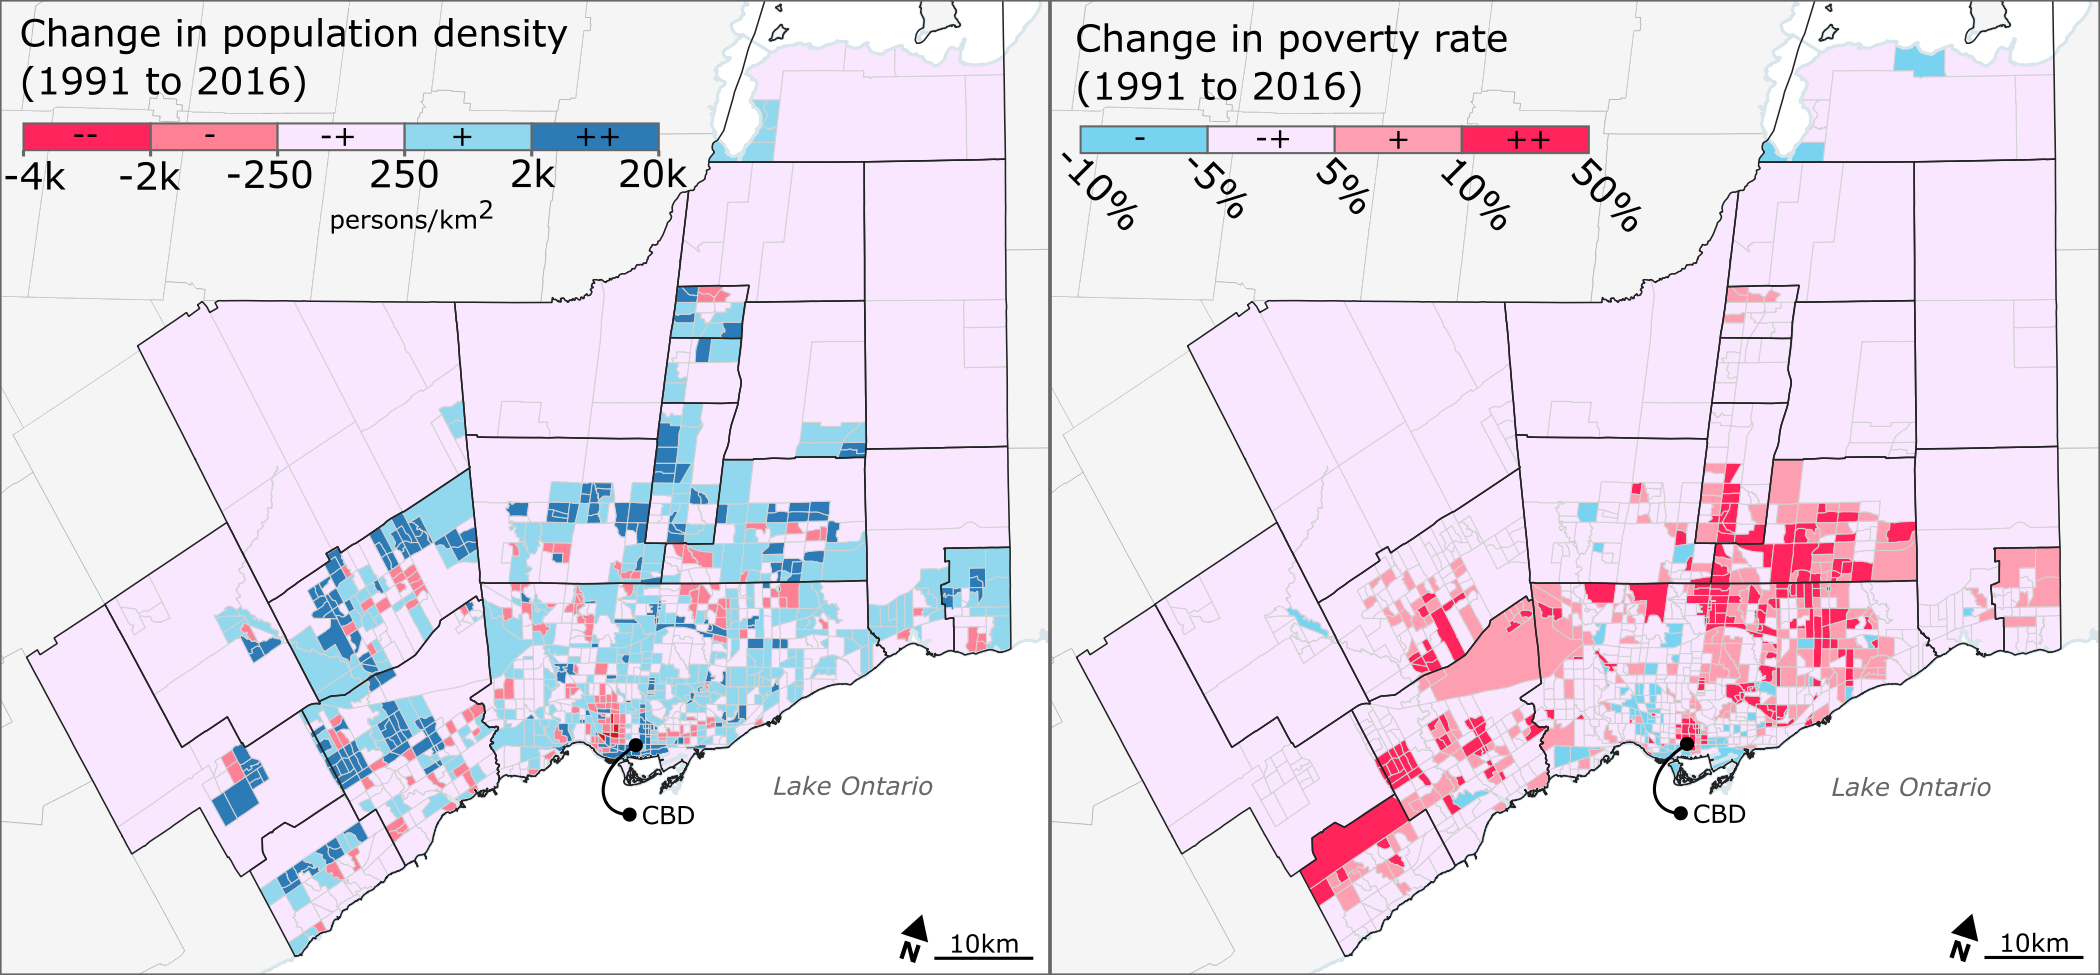
\includegraphics[width=1\linewidth]{figures/study_area_map.png}
	\caption{{Changes in population density and poverty rates in the Toronto CMA (1991 to 2016)}}
	\label{fig:studyareamap}
\end{figure}


While the automobile is the primary mode for most residents in the Toronto CMA (68\% of commuting trips in 2016 were by car), public transit is used by many for daily travel (24\% of commuting trips in 2016) and especially by lower-income residents (32\% of commuting trips in 2016 by low-income workers were by public transit) \cite{government_of_canada_2016_2016}. The Toronto CMA is an agglomeration of several municipalities, each of which operate their own public transit agency, primarily consisting of surface bus routes. The Toronto Transit Commission, the largest municipal transit agency in the region additionally operates surface streetcar routes and a four-line grade-separated rapid transit network. During the time period of our study (1988-2018), the rapid transit network expanded from 3 to 4 lines with a total of 11 new rapid transit stations opening, bringing the total up to 75 stations in the network by 2018. There is also a network of commuter rail and regional bus lines operated by GO Transit, the lone regional transit agency. The 7 commuter rail lines are radially configured, focused on commuting trips to and from the downtown central business district. Several of these lines have undergone expansion from only offering peak-period commuting services to all-day two-way service over the past 25 years. Overall, transit accessibility in the Toronto CMA has been found to be vertically equitable in the sense it serves lower-SES residents more than higher income residents, on average \cite{deboosere_evaluating_2018,allen_sizing_2019}. However, an analysis of neighbourhood socio-economic change relative to transit accessibility and travel behaviour has found that growing poverty in suburban neighbourhoods with low transit accessibility is correlated with increasing adverse travel behaviour outcomes such as decreasing activity participation rates and longer commute times \cite{allen_suburbanization_2021}. 





\section{Data Sources}

The two main sources of data for our study are historical neighbourhood-level transit accessibility measures and individual-level panel data that include variables on residential location and household income. 

Place-based measures of potential accessibility, originally formalized by Hansen \cite{hansen_how_1959}, are commonly used to assess the socio-economic distributions of the benefits derived from transport networks and land-use within a region and over time \cite{manaugh_who_2012,pereira_future_2019}. Place-based measures of transit accessibility for our study were based on the following commonly used potential accessibility formulation \cite{hansen_how_1959,levinson_towards_2020}

\begin{equation}
A_{i,t} = \sum_{j \in J} O_{j,t} f(c_{i,j,t})
\end{equation}
\vspace{2mm}

Where $A_{i,t}$ is the accessibility measure for zone $i$ and year $t$, $j \in J$ are the set of destination zones in a region, $c_{i,j,t}$ is the travel cost from zone $i$ to zone $j$, and $O_{j,t}$ is the number of opportunities in a zone, $j$. For our study, we make use of place-based transit accessibility measures that were computed in a previous study that assessed changes in transit accessibility over time in relation to suburbanization of poverty in Toronto from 1991 to 2016 \cite{allen_suburbanization_2021}. These measures were generated from historical travel survey data and travel demand models. Specifically, data on the location of opportunities, $O_{j,t}$ were from quinquennial (1991, 1996, 2001, 2006, 2011, 2016) regional travel survey that represent 5\% of the region's population \cite{ashby_transportation_2016}, and $c_{i,j,t}$ were travel times based on associated retrospective travel demand models \cite{tmg_gtamodel_2016}. The accessibility measures include consideration for both employment and non-work (e.g. discretionary) activity destinations. See \citeA{allen_suburbanization_2021} for further details on these historical transit accessibility measures. Accessibility measures are provided on a scale ranging from 0 to 100 (the maximum value across all years). For our study, we then additionally use linear interpolation to estimate transit accessibility for intermediary years resulting in having transit accessibility measures, $A_{i,t}$, for each census tract, $i$, and every year, $t$, from 1991 to 2016. (Figure \ref{fig:accessmaps} shows transit accessibility measures for 1991 and 2016). Years 1988, 1989, and 1990 are additionally given the values for 1991, and 2017 and 2018 are given the values from 2016. 

This set of transit accessibility measures are then linked to an individual-level panel dataset, the Longitudinal Administrative Databank (LAD). This data is a 20\% sample of tax filers across Canada on an annual basis from 1988 to 2018 \cite{government_of_canada_longitudinal_2020}. Because of privacy issues, the data are accessed at a secure Research Data Centre operated by Statistics Canada. Included in the data are variables on demographics, household composition, low-income status, sampling weights (used for all subsequent analysis), as well as the census tract and postal code of a person's home address on December 31st of each year. We use this geographical information to link the individual data to accessibility measures based on their year, $t$, and census tract, $i$. Importantly, the data also include a dichotomous indicator of low-income status, specifically the Low-Income Measure (LIM). This is a poverty line created by Statistics Canada, defined as half of the adjusted median household in a region, where adjusted is based on the median household income divided by the square root of household size. This accounts for how as a household increases in size, it's monetary needs increase, but at a decreasing rate \cite{government_of_canada_longitudinal_2020}. For our analysis, we term residents under this threshold as "low-income" and those above as "non-low-income"

\begin{figure}[H]
	\centering
	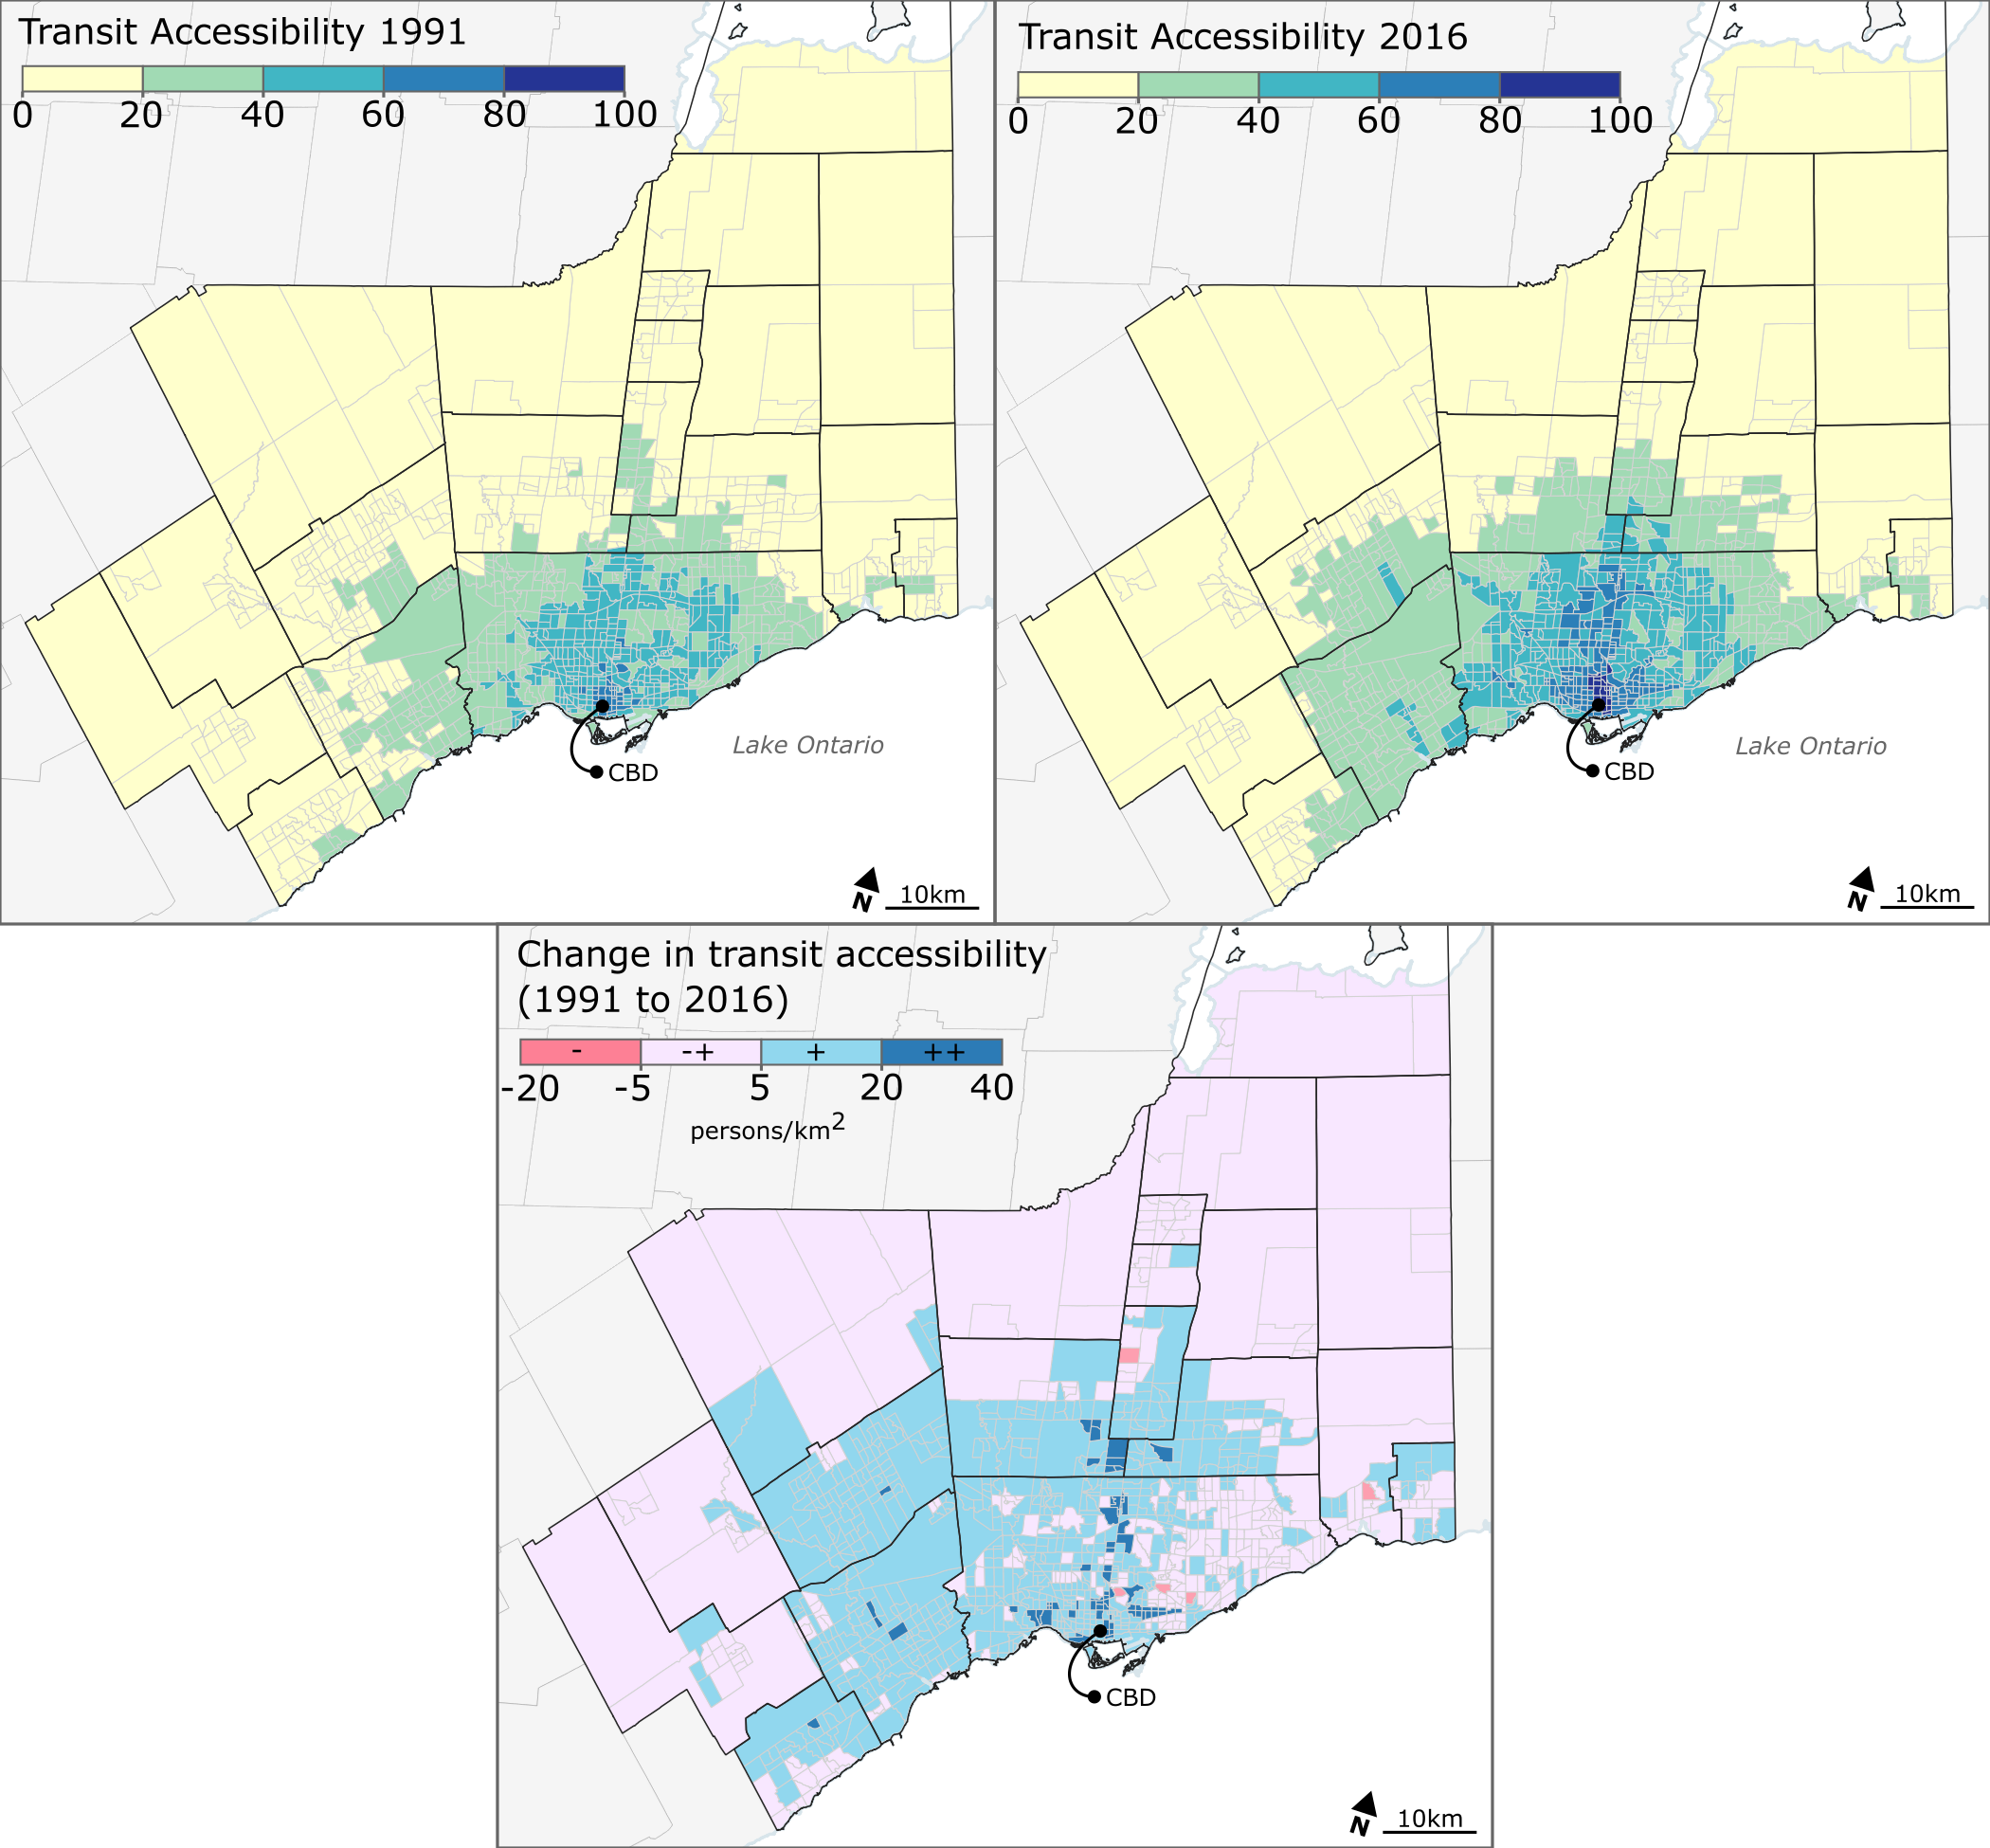
\includegraphics[width=1\linewidth]{figures/acces_mapas.png}
	\caption{{Transit accessibility in Toronto CMA in 1991 and 2016}}
	\label{fig:accessmaps}
\end{figure}



Figure \ref{fig:4plots} displays summary statistics of the Longitudinal Administrative Databank from 1989 to 2018. We find that the poverty rate (\% of the weighted sample in a below LIM household) has increased over time, from approximately 10\% in 1989 to over 20\% 2014, and then declined from 2014 to 2018. The percentage of people who have moved per year has declined over time.  residents move more often than non-low-income households, but this gap has also reduced over time, primarily due to a faster drop in moving rates for low-income residents. Average transit accessibilities have generally increased over time. This is likely due to population growth in areas with good transit accessibility (e.g. downtown) and that most new suburban neighbourhoods have been connected with local bus routes. In some suburban municipalities, there has also been growth in employment which has helped to increase accessibility in nearby neighbourhoods. The data also show that low-income residents, on average, have higher levels of transit accessibility than non-low-income residents throughout this time period.


\begin{figure}[H]
	\centering
	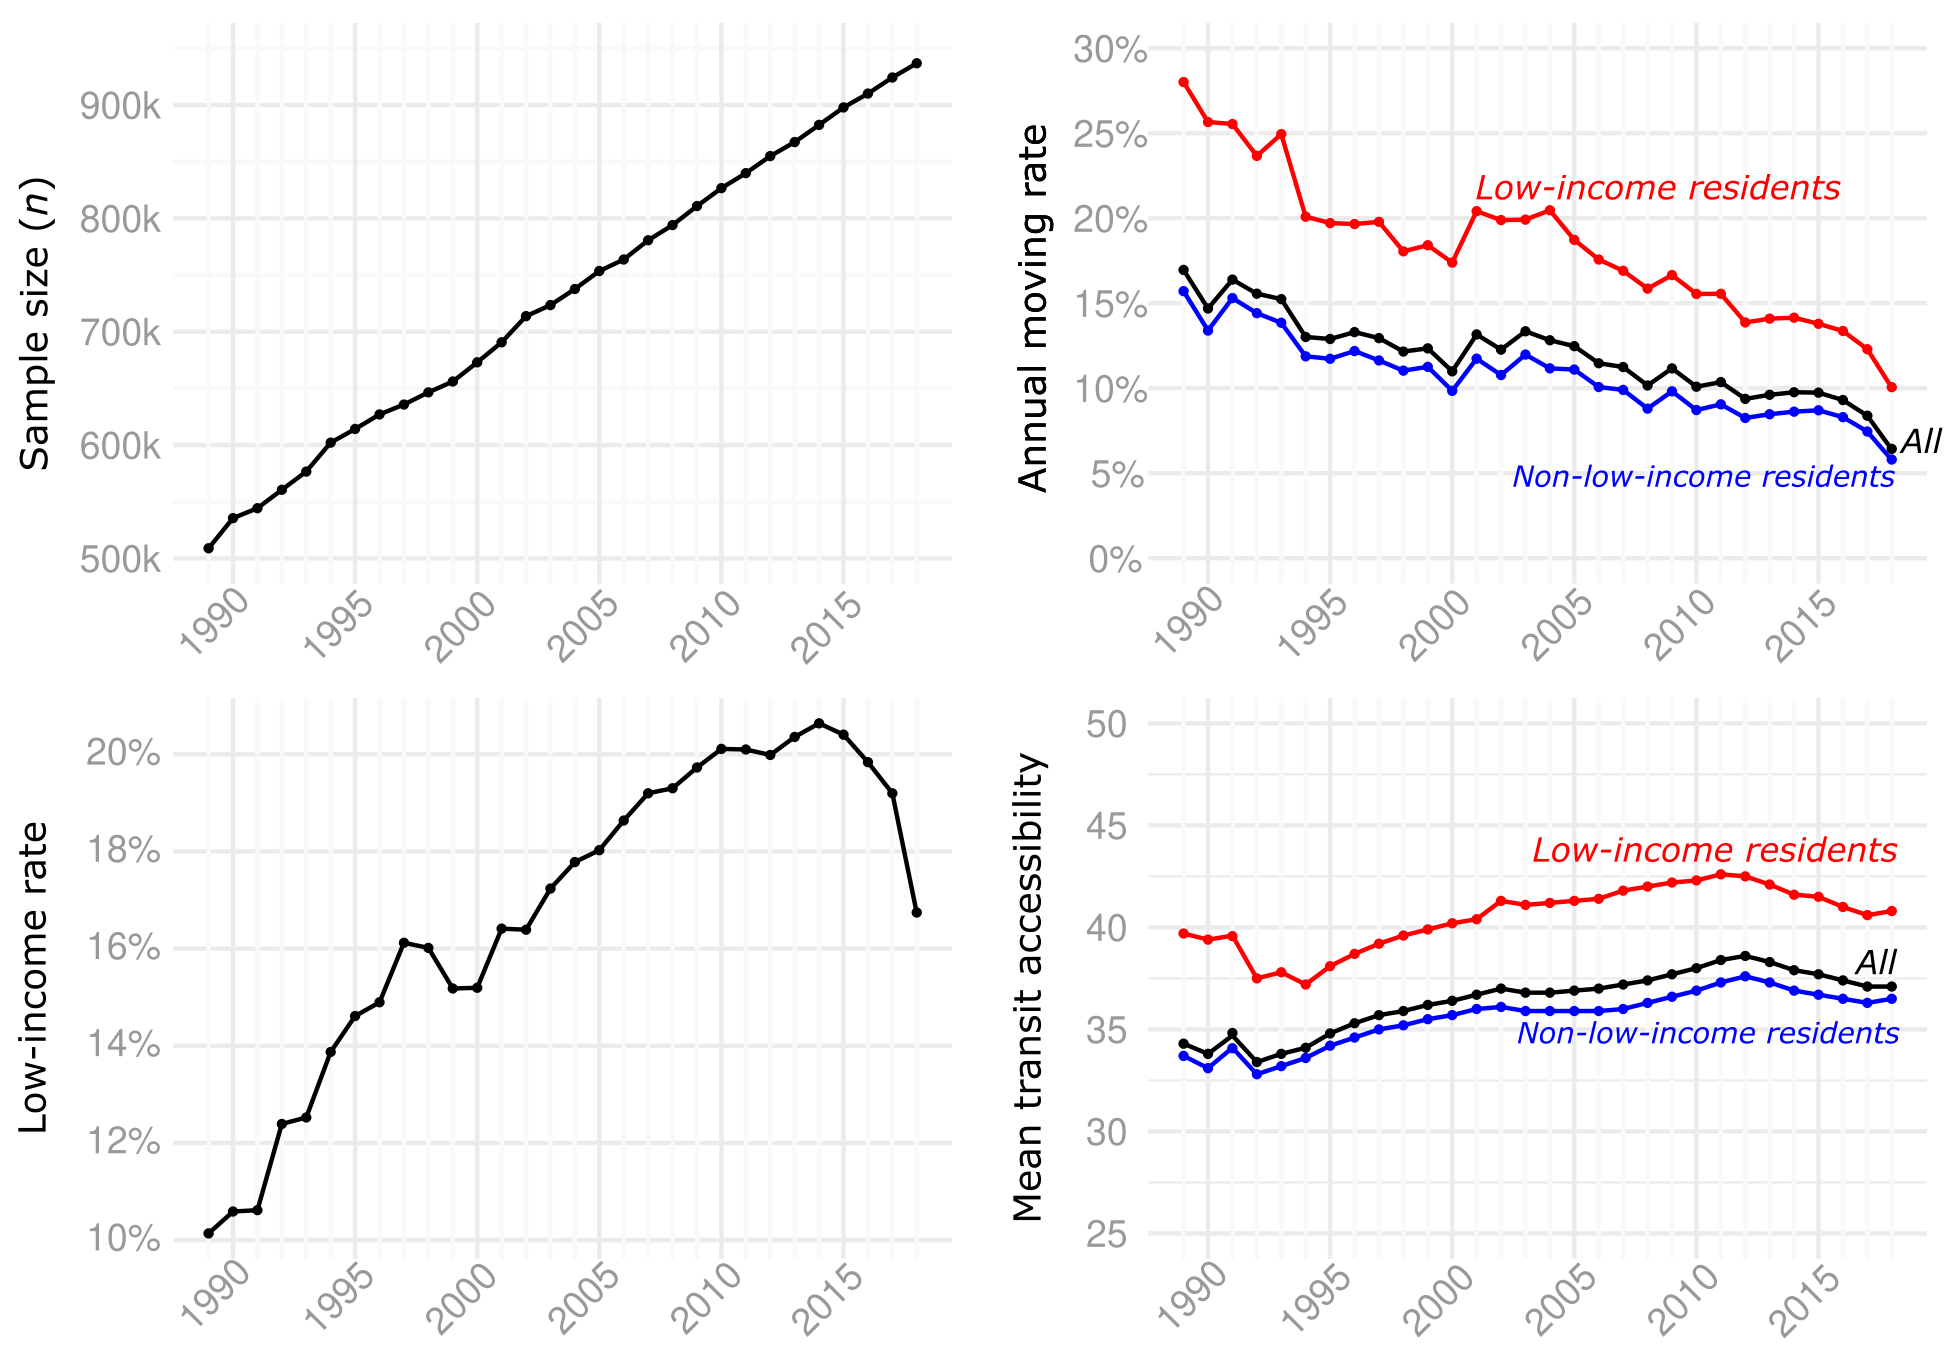
\includegraphics[width=1\linewidth]{figures/4plots.png}
	\caption{{Summary plots of the Longitudinal Administrative Databank and transit accessibility over time}}
	\label{fig:4plots}
\end{figure}




\section{Methods}


From this linked data, we classify whether someone moves if their postal code changes between year $t$ and year $t + 1$. We then compute the absolute difference in transit accessibility, $\Delta A_{k}$, between two years for each mover, $k$, as follows.
\begin{equation}
\Delta A_{k} = A_{i,k,t + 1} - A_{i,k,t}
\end{equation}

A positive value of $\Delta A_{k}$ indicates that a resident has increased their transit accessibility during a move, while a negative value indicates a decrease in transit accessibility. 

For our results, we first create summary statistics and visualizations to show differences in $\Delta A_{k}$ by income status, as well as how this has changed over time. 

We then estimate multivariate regression models to examine if low-income movers are more or less likely to reduce their transit accessibility after controlling for other demographic and household factors that may influence residential mobility to and from different types of neighbourhoods. Because low-income residents have a greater propensity to move (see Figure \ref{fig:4plots}), we use a two-step Heckman selection model to account for how movers are a non-random sample of the overall population. Heckman selection models were initially developed for estimating wages first through labour force participation \cite{heckman_shadow_1974}. In urban transportation research they have been used for analyzing the affects of car ownership and transit accessibility on earnings \cite{smart_disentangling_2020}, analyzing travel distances based on mode choice \cite{kaplan_walking_2016}, and residential moving distances if moved away from new transit infrastructure \cite{chu_impacts_2017}.

The model consists of the following unobserved processes; a selection equation and an outcome equation.
\begin{equation}
m_k^* = \gamma Z_k  + \epsilon_{k,1}
\end{equation}
\begin{equation}
\Delta A_{k}^* = \beta X_{k} + \epsilon_{k,2}
\end{equation}

Where $m_k^*$ and $\Delta A_{k}^*$ are the latent variables for selecting to move and experienced changes in accessibility resulting from a move, respectively, $Z_k$ and $X_{k}$ are vectors of independent variables, $\gamma$ and $\beta$ vectors of coefficients, and  $\epsilon_{k,1}$ and $\epsilon_{k,2}$ are the error terms. In our data, we observe whether people move, and if so, their changes in accessibility. 
\begin{equation}
m_k = 
\begin{cases} 
0 \hspace{1mm} \text{if} \hspace{1mm} m_k^* < 0 \\
1 \hspace{1mm} \text{otherwise}
\end{cases}
\end{equation}
\begin{equation}
\Delta A_{k}  = 
\begin{cases} 
0 \hspace{7mm} \text{if} \hspace{1mm} m_k = 0 \\
\Delta A_{i,k}^* \hspace{1mm} \text{otherwise}
\end{cases}
\end{equation}

The selection equation is modelled as a binomial probit and the outcome as ordinary least squares regression based on the following assumptions.
\begin{equation}
\epsilon_{k,1} \sim N(0,1)
\end{equation}
\begin{equation}
\epsilon_{k,2} \sim N(0,\sigma)
\end{equation}
\begin{equation}
corr(\epsilon_{k,1},\epsilon_{k,2}) = \rho 
\end{equation}

Because of this assumed correlation, the outcome equation includes the inverse Mills ratio based on the linear predictions from the probit selection equation as an additional variable in the outcome equation. The model is estimated via maximum likelihood using the \texttt{sampleSelection} library in $R$. For additional details on model estimation, see Toomet and Henningsen \cite{toomet2008sample}. Models are generated for data from all years pooled into a single dataset, and include a categorical variable for year (this is categorical rather than numeric due to the non-linear temporal relationships shown in the previous plots). Importantly, the independent variables, $X$ and $Z$, include a categorical variable for low-income status. The direction and significance of its coefficient will convey whether low-income residents are more or less likely to reduce their transit accessibility when they move. 


% The expected value for the outcome equation is written as follows:


% \begin{equation}
% E[\Delta A_{i,k} | X_k, m_k = 1] = \beta X_{k} + \rho \sigma \lambda (\gamma Z_k)
% \end{equation}


To round up our study, we categorize transit accessibility into 10 groups (ranked from low to high) using equal intervals (e.g. the lowest is 0-10, the highest is 90-100). We then count how many movers, $N_{u,v,w}$, have moved between different transit accessibility of category, $u$, to category, $v$, by income status, $w$ (i.e. for low- and non-low-income residents) during the study period. Visualizing these flows by accessibility category and income group allows for examining how the more aggregate trends from the previous analyses are possibly due to proportionately low or high out-mobility for each income group or due to residential exclusion at different locations along the spectrum of transit accessibility.




\section{Results}

We begin by visualizing mean changes in accessibility experienced by intra-urban movers. This is shown in Figure \ref{fig:2smooth}. The left figure plots the percent of residents who decrease their levels of transit accessibility when they move. The right figure plots the average change in accessibility, $\Delta A_{k}$, experienced during an intra-urban move. The dashed lines are the means across the entire time period, while the solid lines are local averages fit with a generalized additive model. Overall, residents decrease their transit accessibility, on average, when they move. Looking at the curves, we see fluctuations over time, which likely pertain to core-periphery development trends over time as well. In the early 1990s, residents were more likely to move towards transit, but since 2000, this has hovered around and slightly above the 50\% mark (more residents are moving away from transit). The curves for $\Delta A_{k}$ are consistently less than 0. This is likely partly due to how the newest built suburban neighbourhoods (that thus primarily consist of people moving in, and not out) have some of the lowest transit accessibility in the region. This also indicates that central housing probably has relatively more in-movers from external migration, while peripheral suburban housing has more residents moving in from within the city and thus undergoing a larger reduction in their level of transit accessibility.


\begin{figure}[H]
	\centering
	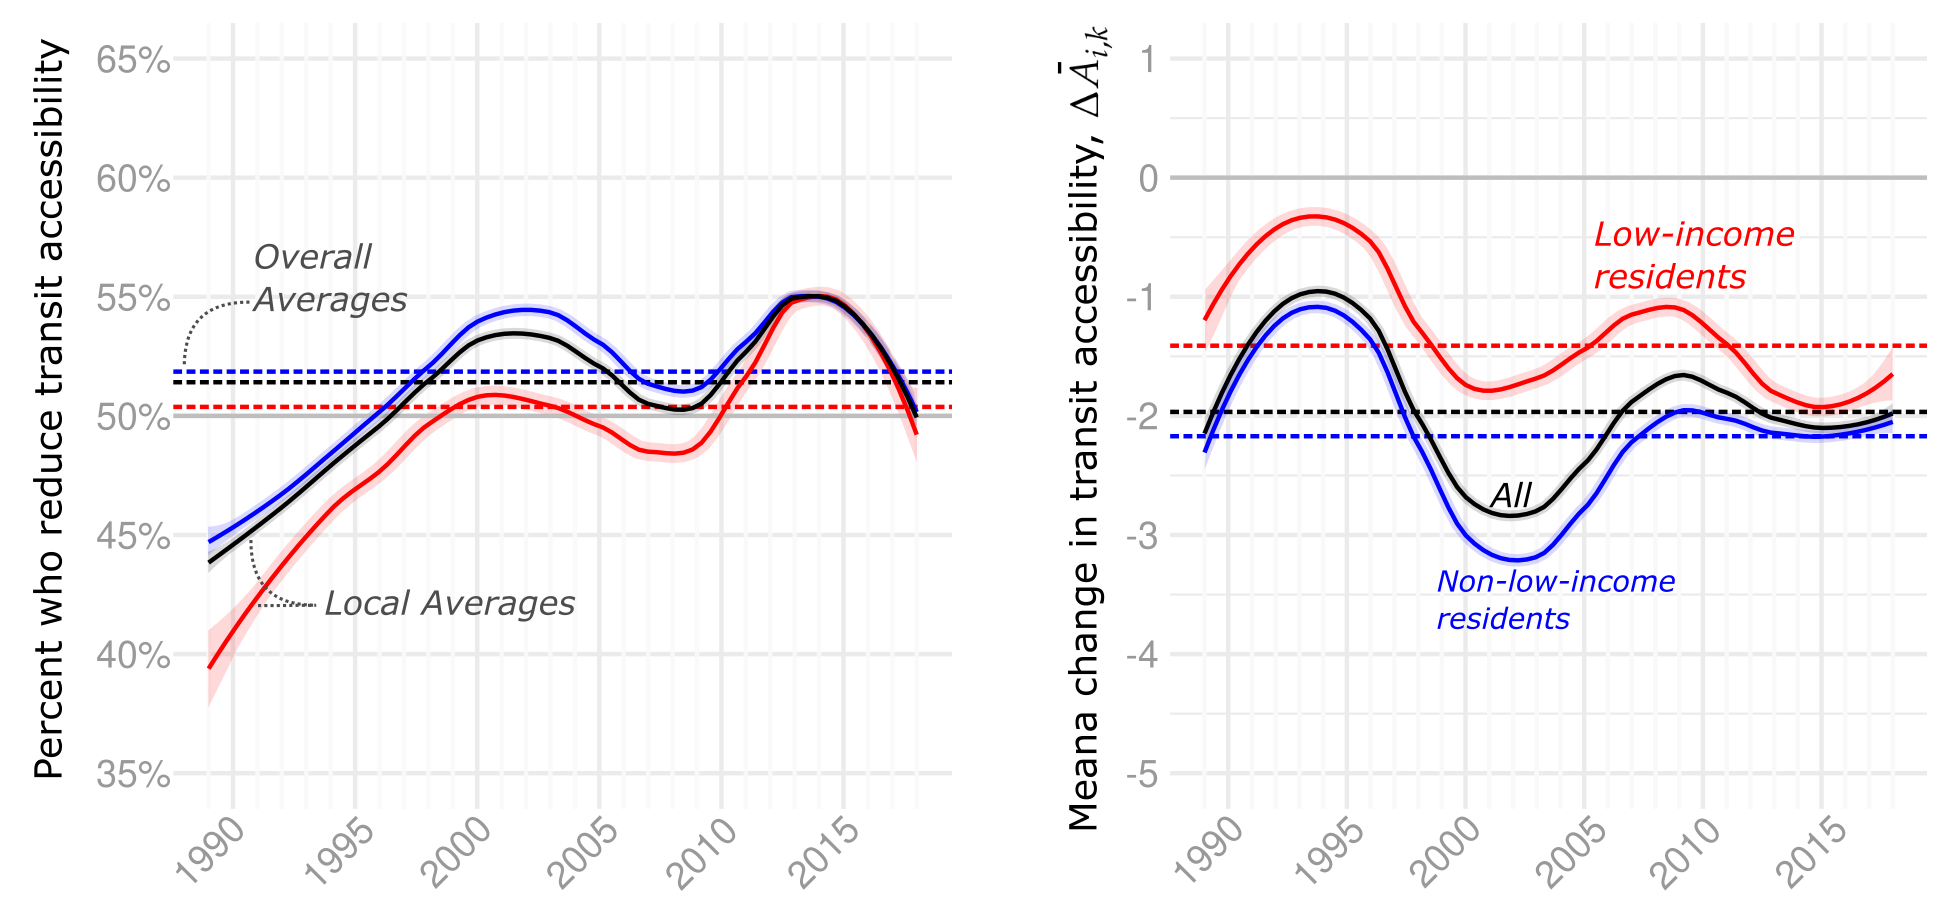
\includegraphics[width=1\linewidth]{figures/2smooth.png}
	\caption{{Changes in transit accessibility for intra-urban movers}}
	\label{fig:2smooth}
\end{figure}

Comparing low-income and non-low-income residents, we find that higher income residents are more likely to decrease their accessibility when moving, and the extent of their reduction is greater as well (the yearly averages are significantly different based on a $t$-test). Therefore, during this study period in Toronto, low-income residents do not decrease their transit accessibility when they move at a greater rate compared to non-low-income residents. However, when looking at the trends over time, we find that the low-income and non-low-income curves converge during the final 10 years of the study period. This is an indication that the effects of gentrification and suburbanization of poverty, at least in terms of residential mobility, are also increasing over time. We find that from 2012 to 2018, low- and non-low-income residents move away from transit at approximately the same rate, but low-income residents still experience less of a reduction in transit accessibility during this time period. This finding could be evidence of residential exclusion in the newest, most peripheral suburbs, as these areas consist of single-family dwellings that are unaffordable for lower-income residents. Also, locations of suburban poverty in Toronto concentrate more within the inner-suburbs, which when viewed regionally, have average levels of transit accessibility. 



These relationships are further examined via the results of regression models displayed in Table \ref{table:models}. Positive coefficients in the selection model ($\gamma > 0$) indicate that the variable has a positive affect on the propensity to move. Confirming the descriptive trends (Figure \ref{fig:4plots}), low-income residents are more likely to move in the past year. Recent immigrants are also more likely to move. Overall this indicates that people living with lower levels of socio-economic status are more likely to experience residential instability and increased propensity to move. Changes in family status, such as having children, children moving in or out, or couples forming or splitting, also increase likelihood of moving, likely due to wanting to change dwellings to suit new household needs.

Positive coefficients in the outcome model ($\beta > 0$) indicate that the variable is more likely to increase the level of transit accessibility during a residential move (each unit increase in $X$ increases transit accessibility by a value of $\beta$ during a move). For low-income status, we find that low-income residents have a change in transit accessibility of 0.84 more than non-low-income residents. Overall, this is not a substantial difference, given that accessibility in this case ranges on a scale of 0 to 100, but still a significant difference. These results also corroborate the descriptive analysis shown in Figure \ref{fig:2smooth}. Aside from income, household factors such as reducing household size, being a lone-parent, being a recent immigrant, and the presence of older children in the household all increase the likelihood of increased transit accessibility when moving. These factors are likely both due to neighbourhood preferences (e.g. for urban neighbourhoods, living near transit) as well as dwelling preferences (e.g. smaller dwelling sizes, which also tend to be more centrally located).



\begin{table}[H]
	
	\renewcommand{\baselinestretch}{1.0} 
	\small
	
	\caption{{Results of Heckman selection models predicting change in transit accessibility for intra-urban movers}}
	\label{table:models}
	
	\begin{adjustwidth}{-1in}{-1in}
		\centering
	\begin{tabular}{lrrrrrrr}
		\hline
		&         &  & \multicolumn{2}{r}{\textbf{Selection Model}}              &                      & \multicolumn{2}{r}{\textbf{Outcome Model}}                \\
		\textbf{Independent Variables$^*$}   &  &  & \multicolumn{1}{c}{$\gamma$} & \multicolumn{1}{c}{$p$} & \multicolumn{1}{c}{} & \multicolumn{1}{c}{$\beta$} & \multicolumn{1}{c}{$p$} \\ \hline
		Intercept                               &         &  & -1.072                   & 0.000                 &                      & -1.289                   & 0.000                 \\
		Income Status in year $t$                   &         &  &                          &                       &                      &                          &                       \\
		\hspace{2mm} Non-low-Income (ref)                         & 82.8\%  &  &                          &                       &                      &                          &                       \\
		\hspace{2mm} Low-Income                                & 17.2\%  &  & 0.186                    & 0.000                 &                      & 0.843                    & 0.000                 \\
		Immigrated between $t - 1$ and $t$             &         &  &                          &                       &                      &                          &                       \\
		\hspace{2mm} No (ref)                                  & 98.6\%  &  &                          &                       &                      &                          &                       \\
		\hspace{2mm} Yes                                       & 1.4\%   &  & 0.284                    & 0.000                 &                      & 0.279                    & 0.000                 \\
		Sex                                       &         &  &                          &                       &                      &                          &                       \\
		\hspace{2mm} Female (ref)                              & 52.3\%  &  &                          &                       &                      &                          &                       \\
		\hspace{2mm} Male                                      & 47.7\%  &  & 0.008                    & 0.000                 &                      & 0.033                    & 0.004                 \\
		Age in year $t$                             &         &  &                          &                       &                      &                          &                       \\
		\hspace{2mm} 18 to 25 (ref)                            & 13.0\%  &  &                          &                       &                      &                          &                       \\
		\hspace{2mm} 26 to 35                                  & 20.3\%  &  & 0.060                    & 0.000                 &                      & -1.180                   & 0.000                 \\
		\hspace{2mm} 36 to 45                                  & 21.3\%  &  & -0.165                   & 0.000                 &                      & -0.974                   & 0.000                 \\
		\hspace{2mm} 46 to 55                                  & 18.0\%  &  & -0.349                   & 0.000                 &                      & -0.520                   & 0.000                 \\
		\hspace{2mm} 56 to 65                                  & 12.7\%  &  & -0.535                   & 0.000                 &                      & -0.312                   & 0.000                 \\
		\hspace{2mm} 66 to 75                                  & 8.6\%   &  & -0.660                   & 0.000                 &                      & -0.097                   & 0.286                 \\
		\hspace{2mm} 76 and up                                 & 6.2\%   &  & -0.587                   & 0.000                 &                      & -0.895                   & 0.000                 \\
		Family type in year $t$                     &         &  &                          &                       &                      &                          &                       \\
		\hspace{2mm} Couple with children                      & 46.9\%  &  &                          &                       &                      &                          &                       \\
		\hspace{2mm} Couple without children           & 24.7\%  &  & 0.171                    & 0.000                 &                      & -0.361                   & 0.000                 \\
		\hspace{2mm} Lone parent           & 8.0\%   &  & 0.198                    & 0.000                 &                      & 1.613                    & 0.000                 \\
		\hspace{2mm} Single/roommates              & 20.3\%  &  & 0.351                    & 0.000                 &                      & 1.792                    & 0.000                 \\
		Number of children in year $t$              &         &  &                          &                       &                      &                          &                       \\
		\hspace{2mm} Children aged 0 to 4                      & $\mu = $ 0.15    &  & 0.069                    & 0.000                 &                      & -0.607                   & 0.000                 \\
		\hspace{2mm} Children aged 5 to 9                      & $\mu = $ 0.16    &  & -0.020                   & 0.000                 &                      & -0.227                   & 0.000                 \\
		\hspace{2mm} Children aged 10 to 14                    & $\mu = $ 0.17    &  & -0.014                   & 0.000                 &                      & -0.058                   & 0.000                 \\
		\hspace{2mm} Children aged 15 to 18                    & $\mu = $ 0.16    &  & -0.116                   & 0.000                 &                      & 0.011                    & 0.597                 \\
		\hspace{2mm} Children aged 19 and up                   & $\mu = $ 0.38    &  & -0.261                   & 0.000                 &                      & 0.316                    & 0.000                 \\
		Change in rel. status between $t$ and $t + 1$ &         &  &                          &                       &                      &                          &                       \\
		\hspace{2mm} No change (ref)                           & 91.2\%  &  &                          &                       &                      &                          &                       \\
		\hspace{2mm} Couple split up                           & 3.0\%   &  & 0.827                    & 0.000                 &                      & 3.823                    & 0.000                 \\
		\hspace{2mm} Became a couple                           & 5.8\%   &  & 0.051                    & 0.000                 &                      & -2.013                   & 0.000                 \\
		New baby in the hhld between $t$ and $t + 1$            &         &  &                          &                       &                      &                          &                       \\
		\hspace{2mm} No (ref)                                  & 97.4\%  &  &                          &                       &                      &                          &                       \\
		\hspace{2mm} Yes                                       & 2.6\%   &  & 0.094                    & 0.000                 &                      & -1.101                   & 0.000                 \\
		Change in children moving in/out from $t$ to $t + 1$        &         &  &                          &                       &                      &                          &                       \\
		\hspace{2mm} No change (ref)                   & 88.7\%  &  &                          &                       &                      &                          &                       \\
		\hspace{2mm} More children moved in                         & 4.5\%   &  & 0.398                    & 0.000                 &                      & -0.894                   & 0.000                 \\
		\hspace{2mm} More children moved out                        & 6.9\%   &  & 0.837                    & 0.000                 &                      & 2.448                    & 0.000                 \\ \hline
		&         &  &                          &                       &                      &                          &                       \\
		\textbf{Model parameters}                  &   $n$   &    & Statistic & $p$                          &                                            &                          &                       \\ \hline
		$\sigma$                                     &         &  & 21.506                   & 0.000                 &                      &                          &                       \\
		$\rho$                                       &         &  & -0.043                   & 0.000                 &                      &                          &                       \\
		$n$ overall                             &           21,821,785  &  &              &                       &                      &                          &                       \\
		$n$ movers                               &            2,512,020 &  &               &                       &                      &                          &       \\ \hline          
		\multicolumn{8}{p{12.2cm}}{\small{$^*$ Categorical variables for year are displayed in Table \ref{table:models_2}}}\\
		
	\end{tabular}
	\end{adjustwidth}
	
\end{table}




\begin{table}[H]
	\renewcommand{\baselinestretch}{1.0} 
	\small
	\centering
	\caption{{Coefficients for year for the Heckman selection models presented in Table \ref{table:models}}}
	\label{table:models_2}
	\begin{tabular}{lrrrrrrr}
		\hline
		&         &  & \multicolumn{2}{r}{\textbf{Selection Model}}              &                      & \multicolumn{2}{r}{\textbf{Outcome Model}}                \\
		\textbf{Year}   &  &  & \multicolumn{1}{c}{$\gamma$} & \multicolumn{1}{c}{$p$} & \multicolumn{1}{c}{} & \multicolumn{1}{c}{$\beta$} & \multicolumn{1}{c}{$p$} \\ \hline
		
		1988 (ref) & 2.3\% &  &                   &                 &  &                  &                \\
		1989       & 2.4\% &  & -0.152            & 0.000           &  & 1.259            & 0.000          \\
		1990       & 2.5\% &  & -0.058            & 0.000           &  & 0.029            & 0.450          \\
		1991       & 2.6\% &  & -0.081            & 0.000           &  & 1.099            & 0.000          \\
		1992       & 2.6\% &  & -0.078            & 0.000           &  & 1.506            & 0.000          \\
		1993       & 2.8\% &  & -0.153            & 0.000           &  & 1.808            & 0.000          \\
		1994       & 2.8\% &  & -0.146            & 0.000           &  & 1.500            & 0.000          \\
		1995       & 2.9\% &  & -0.124            & 0.000           &  & 1.177            & 0.000          \\
		1996       & 2.9\% &  & -0.130            & 0.000           &  & 0.727            & 0.000          \\
		1997       & 3.0\% &  & -0.167            & 0.000           &  & 0.483            & 0.000          \\
		1998       & 3.0\% &  & -0.142            & 0.000           &  & -0.109           & 0.017          \\
		1999       & 3.1\% &  & -0.211            & 0.000           &  & -0.167           & 0.001          \\
		2000       & 3.2\% &  & -0.102            & 0.000           &  & -0.434           & 0.000          \\
		2001       & 3.3\% &  & -0.093            & 0.000           &  & -0.498           & 0.000          \\
		2002       & 3.3\% &  & -0.087            & 0.000           &  & -0.313           & 0.000          \\
		2003       & 3.4\% &  & -0.094            & 0.000           &  & -0.257           & 0.000          \\
		2004       & 3.4\% &  & -0.116            & 0.000           &  & 0.108            & 0.015          \\
		2005       & 3.5\% &  & -0.163            & 0.000           &  & 0.152            & 0.002          \\
		2006       & 3.6\% &  & -0.169            & 0.000           &  & 0.527            & 0.000          \\
		2007       & 3.6\% &  & -0.230            & 0.000           &  & 0.758            & 0.000          \\
		2008       & 3.7\% &  & -0.167            & 0.000           &  & 0.649            & 0.000          \\
		2009       & 3.8\% &  & -0.228            & 0.000           &  & 1.033            & 0.000          \\
		2010       & 3.8\% &  & -0.208            & 0.000           &  & 0.549            & 0.000          \\
		2011       & 3.9\% &  & -0.274            & 0.000           &  & 0.057            & 0.321          \\
		2012       & 4.0\% &  & -0.250            & 0.000           &  & 0.173            & 0.002          \\
		2013       & 4.0\% &  & -0.239            & 0.000           &  & 0.386            & 0.000          \\
		2014       & 4.1\% &  & -0.246            & 0.000           &  & 0.355            & 0.000          \\
		2015       & 4.2\% &  & -0.266            & 0.000           &  & 0.256            & 0.000          \\
		2016       & 4.2\% &  & -0.331            & 0.000           &  & 0.227            & 0.000          \\
		2017       & 4.3\% &  & -0.612            & 0.000           &  & 0.799            & 0.000 
		\\ \hline
	\end{tabular}
\end{table}






In the results in Figure \ref{fig:2smooth} and Table \ref{table:models}, we find that low-income residents are less likely than high income residents to decrease transit accessibility when moving. To provide further nuance into these findings, we first plot the percent of residents by income group moving out of different intervals of transit accessibility during the study period (Figure \ref{fig:res_acc_inc} left). This shows that in the highest accessibility areas, non-low-income residents are more likely to move out compared to non-low-income residents the lowest accessibility neighbourhoods. The trend is different for low-income residents, who move out less often in the highest and lowest accessibility areas, but move more out of neighbourhoods in the middle of the accessibility spectrum (these neighbourhoods approximately correspond to the inner-suburbs, and the greater percents in inner suburbs may be due to the high concentrations of recent immigrants in some of these neighbourhoods). Overall, these results indicate that despite trends of gentrification in areas of high transit accessibility, low-income residents are not moving out at a disproportionate rate. This finding is similar to those in the United States \cite{freeman_displacement_2005,delmelle_new_2020}. 

Figure \ref{fig:res_acc_inc} (right) shows the percent of in-movers into each interval of transit accessibility by income group. This plot indicates that the areas of the lowest accessibility, i.e. rural areas, exurbs, and peripheral suburbs are more exclusive for non-low-income residents - rather than middle or high accessibility neighbourhoods. Overall, non-low-income residents having a greater propensity to move out of high-accessibility neighbourhoods and into the lowest-accessibility neighbourhoods is a key reason why they decrease their transit accessibility when moving more than low-income residents.


\begin{figure}[H]
	\centering
	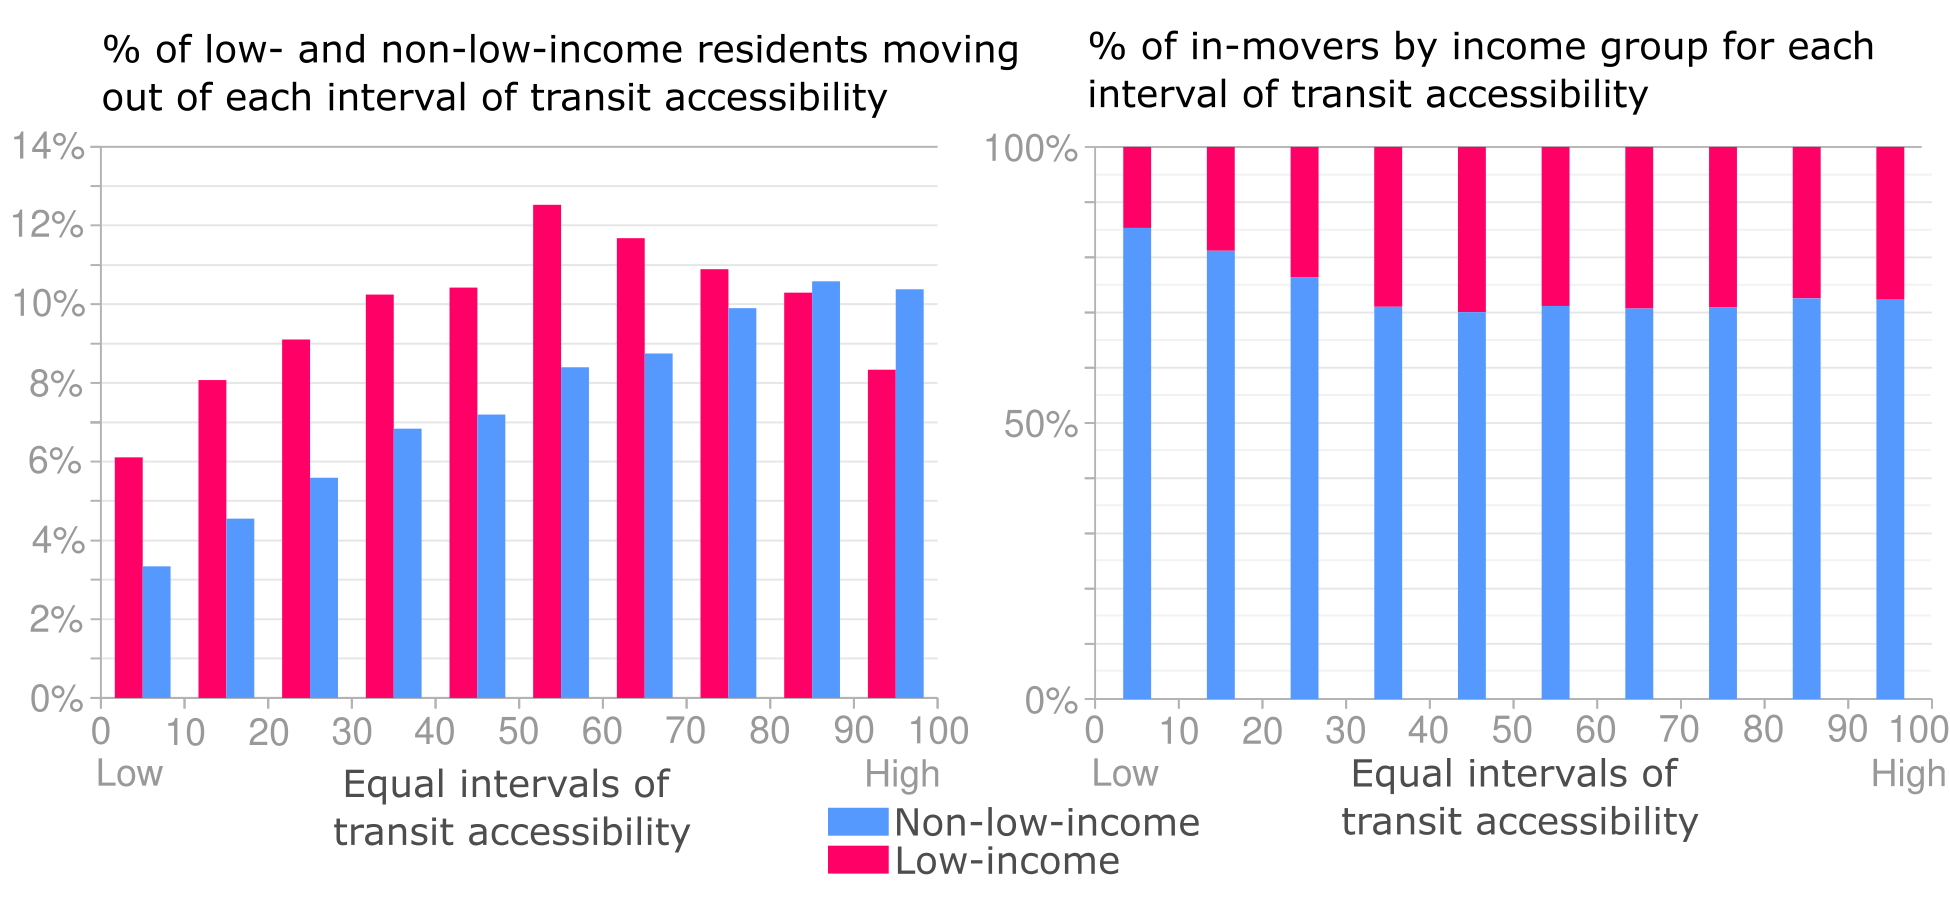
\includegraphics[width=1\linewidth]{figures/res_acc_inc_bars.png}
	\caption{{In and out movers by income and equal intervals of transit accessibility}}
	\label{fig:res_acc_inc}
\end{figure}





\section{Conclusions}

In our analysis, we find that low-income residents, on average, decrease their transit accessibility when they move. This has important social inclusion implications since many low-income residents are reliant on public transit for travelling to daily activities \cite{allen_planning_2020,barri_can_2021}, including finding employment \cite{fransen_relationship_2019,bastiaanssen_does_2021}. Moving away from relied upon public transit could thus decrease capabilities for activity participation, and in some cases, increase risks of transport-related social exclusion \cite{lucas_transport_2012,allen_planning_2020}.

However, we also find that low-income residents do not decrease their transit accessibility when moving at a greater rate than non-low-income residents. This is despite ample neighbourhood-level research describing inner-city gentrification occurring in Toronto over the past several decades \cite{hulchanski_three_2010,walks_gentrification_2021}. In fact, we find that non-low-income residents living in central areas are more likely to move out of these neighbourhoods than compared to low-income residents, and on average experience greater reductions in their levels of transit accessibility when they move. This difference in findings is likely because the unit of analysis of our study were individuals rather than neighbourhoods, meaning that gentrification observed at a neighbourhood level is likely partly due to upward income mobility of residents who stay in these neighbourhoods or affluent residents moving in from outside the study region (either national or international immigrants). As well, we also find that much of the outward residential mobility by non-low-income households noted in 20th century urban theory \cite{burgess_growth_1925,alonso_location_1964} has continued to persist in Toronto. In particular, the outer suburbs and exurbs of Toronto are predominately exclusive to non-low-income residents compared to other areas. 

Even though low-income residents are not disproportionately moving away from transit relative to non-low-income residents, gentrification and increasing costs of housing are still likely leading to changing spatial patterns of low-income neighbourhoods in the region. In Toronto, the most affordable housing is located in the inner-suburbs as mid-20th century apartment towers \cite{skaburskis_filtering_2014,august_gentrification_2018}. The formation of low-income neighbourhoods in these inner-suburban neighbourhoods, but without evidence of substantial displacement and residential exclusion in central neighbourhoods, indicates that these observed increases in suburbanization of poverty in Toronto is more likely due to immigrants with lower incomes settling in the suburbs or residents becoming and remaining poor in-place within the suburbs.

Overall, it would be difficult to generalize the findings from our analysis to other regions. However, the methods we presented could be replicated elsewhere. This would certainly be doable in other Canadian contexts as the panel dataset we used is available Canada-wide \cite{government_of_canada_longitudinal_2020}, but it would require additional sources for historical transit accessibility measures elsewhere (we only had this data available for Toronto). Conducting a comparative analysis across multiple cities would be an important direction for future work to assess whether there are consistencies or differences in findings regarding whether low-income residents are unequally moving away from transit. Similarly, future research could examine how results might vary using different definitions of accessibility and thresholds for low-income status, possibly as part of a sensitivity analysis. For example, our historical travel survey data were limited in that we could only look at access to all jobs within a region, rather than low-income jobs. Moreover, while the objective of our study was to examine changes across an entire region, another important direction for future work would be to map at a more localized scale whether there are neighbourhoods that have undergone high rates of out-mobility of low-income residents, and specifically if out-movers are decreasing their transit accessibility when moving, even if these trends are not prevalent at an aggregate regional level. This could provide more direct evidence into the locations within a region that are potentially experiencing residential displacement away from relied-upon public transit service.




\chapter{Conclusions}
\label{ch:conc}

\section{Research Contributions}

The overarching goal of this dissertation was to analyze trends of growing rates of poverty in the suburbs of Canadian cities during the late 20th and early 21st centuries; and how this affects daily travel, activity participation, and social inclusion. Chapter \ref{ch:background} provided a background and discusssion of previous research on the related issues and three innovative empirical analyses (Chapters \ref{ch:subtrapov}, \ref{ch:pathsubpov}, \ref{ch:lowinctra}) QQQQ insight into BLAH

% problem
Chapter \ref{ch:subtrapov} is motivated by how a potential negative impact of suburbanization of poverty is that lower-income households are re-locating to areas that are more auto-oriented, less walkable, and have relatively lower levels of public transit service than central areas. This could be resulting in longer commutes and increased barriers to daily activity participation, especially for those who are unable to afford a private vehicle. The ability to travel to important activity destinations is vital for economic independence (e.g. finding and retaining employment), health, and well-being - and at a greater scale, it can contribute to robust urban economies and healthier societies as a whole. In the worst cases, dissuasion or inability to travel to important destinations can limit activity participation, result in social exclusion, and negatively impact the vitality of urban environments \cite{lucas_transport_2012,martens_transport_2016}. However, previous research on suburbanization has not considered it's relation to transportation and travel behaviour beyond brief discussion that it is a potential impacat \shortcite<e.g.>{hulchanski_three_2010,walks_social_2001,ades_are_2012,breau_pulling_2018, grant_changing_2020}. 

Accordingly, in this chapter combines data sources to analyze the relationships between increasing socio-spatial inequalities (e.g. de-centralization of low-income households), transport disadvantage (e.g. spatial distribution of zero-car households, low levels of transit accessibility), and adverse travel behaviour outcomes (e.g. lengthier commute times and lower activity participation rates). Using methods include computing transit accessibility metrics that are comparable over time, statistical mapping, modelling changes in travel behaviour over time, and visualizing neighborhood change with respect to levels of suburbanization. In paticulary, the spatio-temporal neighbourhood modelling is a quantitative strategy that has not been used in neighbourhood studies in Canada. So while focused on Toronto, these methods can certainly be transferable to other regions where there is available data.

In terms of findings, this study provides solid evidence that transport poverty in Toronto is increasing more in the suburbs relative to central areas. Eastern suburbs in particular have suffered the most, indicative by having the greatest combination of increased transport and social disadvantage, and evidenced by increasing commute times and declining daily activity participation rates. Our research thus confirms theoretical pathways of transport poverty \cite{lucas_transport_2012}, and moreover, shows that it is occurring more within suburban neighbourhoods.

% then lead into next, highlight importance of individual
However, this Chapter (\ref{ch:subtrapov}), like most previous studies analyzing suburbanization of poverty and neighbourhood change more generally \cite{ades_are_2012,breau_pulling_2018,grant_changing_2020} were based on neighbourhoods. But neighbourhood-level analysis could be masking individual effects since we only analyzed change at a neighborhood level. For example, there could be more extreme levels of travel be outcomes in later years than earlier years in certain neighborhoods. Nor is it known whether upward or downward socio-economic status in a neighbourhood is primarily due to residential mobility or residents becoming poorer or wealthier in-place.

As such, the next two Chapters (\ref{ch:pathsubpov} and \ref{ch:lowinctra}) make use of individual-level panel data, specifically the Longitudinal Admininstrative Databank (LAD), a panel dataset of annual tax filers, to examine intra-urban moves relative to transportation and urban form.

Chapter \ref{ch:pathsubpov} is particularly motivated by how ample research (includuing Chapter \ref{ch:subtrapov}) has described trends of suburbanization of poverty at regional and neighbourhood levels, but has been unable to discern how residents end up to become poor and living in the suburbs. This Chapter first develops a conceptual framework describing different potential pathways to suburban poverty, and then uses the LAD to quantify these pathways across urban regions in Canada. This analysis specifically estimates for the first time in Canada to what extent suburban poverty stems from intra-urban residential mobility, external immigration, and remaining poor in-place---thus providing an important link between theory and empirical evidence on the urban dynamics that lead to suburbanization of poverty. Understanding the propensity of these pathways provides important knowledge regarding the urban dynamics that lead to contemporary suburban geographies of poverty concentration. Such knowledge can also be helpful for planning and policy including (but not limited to) public transit prioritization, providing resources for recent immigrants, protections against displacement, and social housing policy; and overall, aiming to reduce the burdens of being poor and living in the suburbs.

This analysis shows that suburban poverty is an increasing phenomenon in Canadian cities. This is evident in our analysis of tax records (see Figure \ref{fig:subpov4}) as well as previous research using census and other survey data \cite{ades_are_2012,breau_pulling_2018,grant_changing_2020,allen_suburbanization_2021}. Importantly, the data indicate that transitioning to suburban poverty on an annual basis is much more a result from staying or becoming poor within the suburbs compared to immigration or due to moving (and potentially being displaced from) gentrifying neighbourhoods in the centre. On a year-by-year basis, of the low-income suburban residents who lived in the suburbs, 21.5\% dropped into poverty while staying in the suburbs on average, compared to only 2.9\% who moved from a central area or the 6.6\% who immigrated from elsewhere. We find that these trends are similar when comparing between regions and over our study period (2006 to 2016). Despite this finding, much of the discussion in Canada on suburbanization of poverty has been directly attributed to gentrification and displacement from less affordable central neighbourhoods \cite{grant_changing_2020}. This points to further consideration into the causes of dropping into poverty in the suburbs including (but not limited to), increasing rents in suburban apartments \cite{august_gentrification_2018}, automobile debt limiting spending in other areas \cite{walks_driving_2018}, or low transit accessibility impacting ability to travel to employment, education, or social services needed for poverty reduction \cite{allen_planning_2020} 

Chapter \ref{ch:lowinctra}, QQQQQ



In conjunction, these three quantitative analyses QQQQQ


% Specifically, we use a combination of census and transportation network data to create a typology of suburbanization via a hierarchical $k$-means cluster analysis. We then link this typology to panel data representing 20\% of tax filers across Canada to examine immigrant settlement patterns and residential mobility trajectories of low-income households, grouped by typologies of suburbanization. 




% Specifically, for those in suburban poverty in Canadian CMAs, 88.5\% lived in the suburbs a year prior (of which, 12.7\% moved residences within the suburbs and 75.8\% did not move), 2.9\% moved from a central neighbourhood, and 6.6\% immigrated from elsewhere (4.6\% internationally, 2.0\% from within in Canada). Moreover, of the low-income suburban residents who lived in the suburbs a year prior, 21.5\% were not classified as being in a low-income in the previous year. Thus becoming poor while staying in the suburbs encompasses a greater proportion of suburban poverty than immigration and \textit{centre}-to-\textit{suburb} mobility combined. 





\section{Implications for Urban Planning}

Policy to reduce these effects should thus have a two-pronged approach. The first is to curb the growth of suburban poverty through focusing on increasing the supply of affordable housing in areas with high transit accessibility, having strong rent controls, and preventing forced eviction and displacement from central to suburban neighborhoods. The second is to upgrade suburban environments through transport planning and urban design strategies that improve transit accessibility and walkability (i.e. improving accessibility at both neighborhood and regional scales). These are not new ideas. Many of them have been advocated for previously in terms of reducing the negative population health and environmental impacts associated with auto-oriented environments \shortcite{cervero_travel_1997,ewing_relationship_2003,ewing_compactness_2015}, and limiting the detrimental impacts suburbanization of poverty has on increasing polarization and segregation of urban space as well as the negative impacts caused by eviction and displacement on individual well-being and community cohesion  \shortcite{hulchanski_three_2010,ades_are_2012,walks_income_2013,august_challenging_2014,august_its_2016}. Our research provides one more important piece of evidence showing that such strategies would also be progressive options in reducing barriers to daily travel and transport-related social exclusion.


Our results also provide pertinent information to aid preventative policy aimed at reducing suburban poverty in Canada. For one, knowledge that a substantial portion suburban poverty stems from becoming poor in-place should expedite support for urban planning and policy to make suburbs more livable and accessible. In other words, policy for reducing suburban poverty should not parochially be focused on other pathways, such as limiting gentrification and displacement. While important to quell such displacement, our findings indicate that it is also imperative to make improvements to the suburbs, such as expanding community and social resources in the suburbs alongside more compact urban design, active travel infrastructure, and improved public transit in order to provide residents the ability to access amenities and opportunities (e.g. employment, education), as these would all be worthwhile strategies aimed at poverty alleviation in the suburbs. Our findings additionally show that international immigrants have a high propensity of settling in the suburbs and being below the poverty line. This points to policy aimed at providing incentives for more housing (e.g. as vouchers) for recent immigrants, particularly in more central locations. 



\section{Data Limitations}

Our study was not immune to limitations, and thus offers directions for future work. For one, our research focused on transport (dis)advantage in terms of transit access to destinations and auto ownership, but we did not consider other components of urban form that could either benefit or detriment urban living. For example, despite gains in transit access, suburban built environments typically remain focused on the car, which have a number of safety and environmental concerns (e.g. speed limits are greater, safe crossings are more spread out, creating barriers to active travel). On the other hand, some suburban areas offer better access to green space, which can have a positive effect on health and well-being. Future research should consider other positive and negative environmental impacts of less-centralized urban living for low-SES populations. This could prove challenging, however, since there is little readily available historic data on urban form, walkability, and access to green space.

Our study also had some other data limitations. We relied on a travel survey that represented a 5\% sample of the population, limiting analysis at smaller geographic scales. Secondly, there may have been some inconsistencies with how data were collected across survey years. We did select variables that were consistently defined over time based on survey documentation, but there were likely some imperfections in interpretation and administration of survey questions. As well, in terms of data, there was likely some inaccuracy caused by the data harmonization process of apportioning data to the same spatial units. These issues are unavoidable when dealing with longitudinal survey data that has been aggregated to different areal units \cite{allen_new_2018}. 

2

This is the first paper that we are aware of that develops a conceptual framework and empirically examines residential mobility pathways to suburban poverty. But given the exploratory nature of our analysis as well as use of a large-sample dataset, we had to make a few simplifications. As such, expanding upon these would also be important directions for future research. First, we used a single binary measure of low-income status (LIM) to classify whether a resident was in poverty in a given year. We used the LIM because it was pre-defined by Statistics Canada as well as used in other research projects \cite{picot_immigration_2014,allen_sizing_2019,brown_money_2019}. However, sensitivity analysis of results for different poverty measures, including those with multiple categories, would allow for more nuanced findings. Similarly, we generated a binary measure via a cluster analysis to describe whether or not a neighbourhood is suburban. This could be expanded to looking at multiple categories of urban form, in particular, specific types of suburban neighbourhoods. The $k$-means hierarchical clustering method we used could certainly be expanded to account for this. As well, other clustering methods could be tested to examine how and to what extent they would affect results.

Our analysis focused on year-to-year transitions from 2006 to 2016. So another important direction for future work would be to analyze individual pathways to suburban poverty prior to 2006 as well as analyze individuals over the course of multiple years. The latter could be conducted via sequence analysis methods to examine whether there are common life-course and residential mobility trajectories to suburban poverty. This could also be used to connect to longer-term neighborhood-level changes (e.g. to ask whether neighbourhoods with more concentrated poverty have a larger share of low-income people who dropped into poverty or who moved from elsewhere?). However, one drawback of using this tax record data is that it lacks contextual factors about why people move. Such factors are difficult to directly infer from tax records. Another direction for future work could be to link this data to possible push or pull factors that may disproportionately affect residential mobility of low-income residents. For example research analyzing out-mobility due to gentrification and new transit infrastructure has been conducted in the United States \cite{freeman_displacement_2005,delmelle_new_2020}, but not in Canada, and nowhere that we are aware of with the sample size of the LAD (20\% of the population). Continuing research in these directions would provide further knowledge regarding the individual pathways and neighbourhood dynamics that lead to suburbanization of poverty.



These problems highlight the need in the future for individual-level linked datasets, similarly to how medical records have been linked to census data in health research. Analyzing individual panel data would be helpful for examining pathways to suburban poverty and whether improvements in transit accessibility are either more likely to alleviate poverty or result in gentrification and displacement.

TTS - to census - make longitudinal if possible - to tax records - to GSS even - other administrative data sources. While there would be privacy concerns, it would be great potential for researchers at the RDC for example


resesarchers
\section{Future Research}

Beyond improving data collection and efforts, this research leads to several directions for additional research.




\subsection{Planning \& Policy Effectiveness}

As noted earlier, the findings of this dissertation have several implications for urban planning and policy, particularly regarding transportation and housing. 

However, this dissertation did not look directly at the effectiveness of any particular project or policy intervention. 

As such, future research could be designed to study the effectiveness of different strategies of reducing the propensity of dropping into poverty in the suburbs.






\subsection{Improving Theory About Urban Dynamics And Activity Behaviour}


% overview
Neighbourhoods are the stage for daily life. Individuals' neighbourhood contexts can impact a number of social outcomes; from daily travel behaviour and activity participation, to longer-term effects on employment, income, health, and well-being \cite{sampson_assessing_2002,ewing_travel_2010,lucas_transport_2012,bastiaanssen_does_2020}. These are often called \textit{neighbourhood effects}. However, environmental contexts change over longer period of time, both in terms of their built environments (e.g. due to land use intensification, transit (dis)investments) and social attributes (e.g. socioeconomic decline, gentrification) \cite{van_ham_understanding_2013,wegener_land-use_2004}. Therefore, one's environmental exposures are not static nor consistent over time, they are sensitive to these \textit{neighbourhood dynamics}. 

Scale, nexus of the individual and the global. 
These longer-term changes are also a product of individual preferences and decisions in aggregate. i.e. neighbourhoods effect individual outcomes, and individuals shape neighbourhoods.


% research goal
The objective of this paper is to present a conceptual framework that synthesizes theories of travel behaviour, neighbourhood effects, and neighbourhood dynamics into a symbiotic whole, one that conveys how neighbourhood effects and neighbourhood dynamics are part of a multi-scalar system of cyclical feedback effects. This is based on combining several related strands of research: 1) research examining environmental effects on daily travel and activity behaviour \cite{hanson_determinants_1982,ewing_travel_2010}; 2) how one's location and preferences impacts resource acquisitions such as housing choices or purchasing a car \cite{lee_neighborhood_1994,klein_millennials_2017}; 3) the effects of prolonged exposures to environments on long-term social outcomes like employment, income, and education \cite{sampson_assessing_2002,chetty_effects_2016}, which are often propagated via feedback effects \cite{wilson_truly_2012,lucas_transport_2012}; and 4) how individual actions, in aggregate, can cause the physical and social characteristics of neighbourhoods to change over time via transport investments, land use change, and residential mobility decisions \cite{wegener_land-use_2004,wilson_truly_2012,van_ham_understanding_2013}. 



In this section, we present a integrated conceptual framework to bring together the aforementioned conceptualizations of how geographic contexts effect individual outcomes, with how these geographic contexts can change over time. 

Why is this important? Implications for research , while controlling , 

human systems, urban systems, are complex - finding order within this complexity ...

The overall framework is shown in Figure 2. This is divided into individual attributes and outcomes, geographic (i.e. neighbourhood) contexts, and global factors. The QQQ lines pertain to effects on individual choices and outcomes, while the QQQ lines pertain to aggregate effects of individuals on neighbourhood and regional characteristics.

Sampson 2019/2012 - cogs micro/macro effects

feedback - lucas

UGCP - Kwan


% social outcomes, such as examining the impacts of changing environmental contexts on travel behaviour \cite{caoChangesNeighborhoodCharacteristics2007},


\begin{figure}[H]
	\caption{Combined conceptualization}
	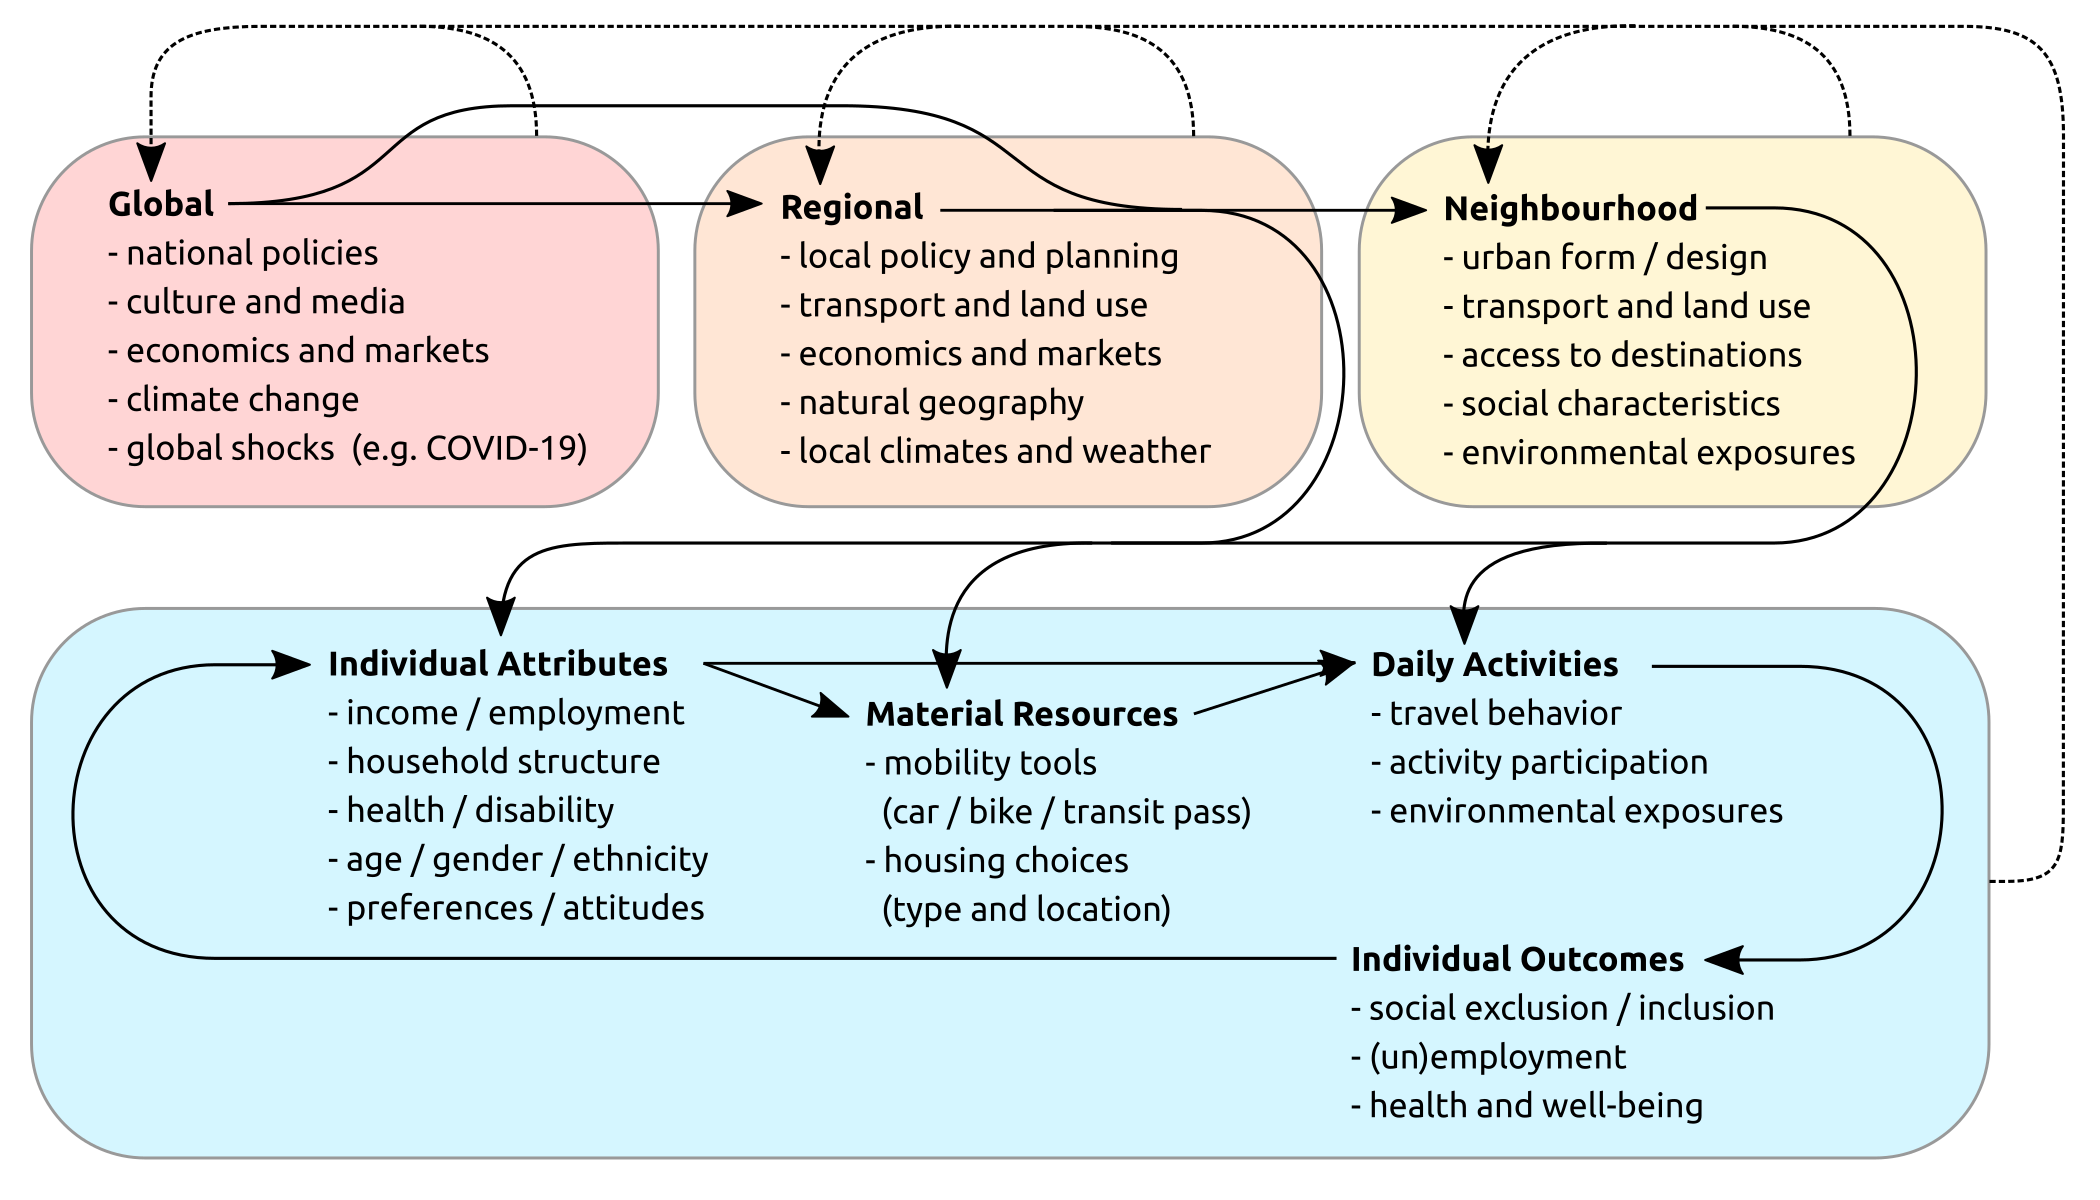
\includegraphics[width=7in]{figures/my_idea.png}
	\centering
\end{figure}




\subsection{Transit-Induced Displacement In Canada}

Beep, expanding upon prev chapter

% transportation urban form income mobility - need data on auto ownership



\subsection{Transit Accessibility, Urban Form, and Income Mobility}

Ample research has shown that compact urban forms and greater levels of transit accessibility promote more environmentally friendly outcomes and healthier lifestyles \cite{ewing_compactness_2015,ewing_travel_2010,cervero_travel_1997}. There are also theoretical arguments that accessibility is a social good, as it enables activity participation \cite{martens_transport_2016,pereira_distributive_2017}.
But what about long-term benefits? Can such built environments also lead to social mobility and poverty reduction? Research has noted how neighbourhood socio-economic effects impact individual social mobility \cite{chetty_effects_2016}, yet research on how urban form, and in particular transit accessibility has on long term social outcomes is sparse \cite{ewing_does_2016,fransen_relationship_2019}.
(I will need to do some more research to see what else has been done with the MOT study and the PSID in the USA, as I think there are a few papers that look at urban form and car ownership on social mobility \cite{smart_disentangling_2020}. There is nothing that I'm aware of in Canada however. There's also quite a few studies that look at the unemployment-accessibility relationship, but few are longitudinal and individual level).

This chapter will use the same data is the previous one, but will attempt to uncover whether low-income residents exposed to more compact urban forms and better levels of transit accessibility have relatively greater income mobility over time relative to areas of worse accessibility, while controlling for other demographic and stage-of-life effects, as well as residential mobility and exposure to different urban forms. In particular, the Longitudinal Administrative Data/Databank/Database (LAD) will be the primary dataset for this paper, as it includes basic demographics (age, gender, marital status) and household structure (info about family members), as well as sources of income included in tax records. One limitation of this data, however, is it does not include information on car ownership, despite it being shown to be related to earnings in the long-term \cite{smart_disentangling_2020}.

For methods, my current thinking is to model change in income, $\Delta I_i$ via a combination of level of accessibility, $A$, urban form, $U$, and controlling for demographic and households characteristics, $X$, and neighbourhood socio-economic variables, $N$.

\[
\Delta I_i = c + \alpha A_i + \mu U_i + \nu N_i + \beta X_i + \epsilon_i
\]

$\Delta I_i$ will be considered first as an absolute value pertaining to after-tax income, scaled to the most recent year's currency value. I will then convert income to measures of equivalent household income, which would then allow for generating measures of poverty based on the LIM methodology\footnote{divide income by the square root of households size, then compare with the distribution of all households. Those less than 50\% of the median are deemed to be under the poverty line}. 
$N$, $A$, and $U$ will be based on one's average if they have moved to over the period of study. It will also be good to add a variable indicating residential mobility. The model will likely require incorporating multilevel effects, for both individual and neighbourhood scales. Spatial effects will be tested at the neighbourhood level. Another modelling option that I'll try to specify is more of an experimental design, where instead of a mean level of accessibility, $A$ and $U$ will be categorical variables pertaining to an increase, decrease, and no-change in accessibility for a specific time period, $t$, caused by a residential mobility event or opening of a new transit line. This strategy could be differentiated or combined for multiple intervention periods.

Overall, the hope is that the sign and significance of the coefficients $\alpha$ and $\mu$ will offer evidence into whether, and to what extent, living in different types of built environments can have on income mobility and poverty reduction. Results will thus provide knowledge about whether and how the built environment (e.g. accessibility and urban form) can be a catalyst for neighbourhood SES change, and how different urban transport planning and design strategies can alleviate poverty.



% future transit accessibility

\subsection{Transportation Forecasting With Urban Dynamics}

Future forecasting with urban dynamics.

Urban futures are rife with uncertainty. Yet when planners and researchers assess the distributions of transit accessibility benefits across different socio-economic groups, they are typically based on current distributions. However, it is clear that the demographic patterns of cities change over time, as recently evidenced by socio-spatial polarization, gentrification, and suburbanization of poverty. As such, transport planners should be mindful of potential socio-economic changes when they examine current and future distributions of transport accessibility, as they can directly relate to social (in)equity and transport-related social exclusion. Accordingly, future research should explore how the distributions of transit accessibility relative to socio-econmoic status can vary substantially depending on different future socio-economic trajectories. Examples of differing trajectories include gentrification versus affordable near transit and polarization versus evenness. 

This could be explored through a theoretical discussion and conceptual examples; simulating data based on current (2016) population, employment, and transit travel time data as base, and apply ranges of outcomes based on the above dimensions. 
SES will be considered as counts of readily available census data such as low-income households by zone, recent immigrants, and other low-SES population groups, likely defined based on my findings in the previous papers. The study area(s) for this part are currently open. I currently have transit travel time data for eight of the largest urban regions in Canada, so any one or more of them could be studied. Simulations will make use of Markov chain Monte Carlo methods, based on stochastic transition matrices generated by parameters relating to polarization-evenness, gentrification-affordability, homophily, and spatial focus of residential mobility. 

Third, I will explore these issues using a regional travel demand model of the Toronto region, specifically by tweaking it's residential mobility sub-model. Access to this model and information of what parameters can be adjusted will require further discussion with the Travel Modelling Group\footnote{\url{https://tmg.utoronto.ca/}} at the Civil Engineering department. The benefit of this approach is that it is a fully integrated model. In other words, it will provide differing outputs for population, land-use, and travel times depending on variation in input parameters. This will allow for computing accessibility measures for multiple scenarios, rather than comparing multiple socio-economic distributions with a single accessibility distribution.

My current expectation is that results will likely indicate that compact urban forms, focused on affordable housing near transit will reap the greatest benefits in terms of social equity and social inclusion.




\subsection{Communication}






\bibliographystyle{apacite}
\bibliography{ref.bib}



%\nocite{*}


\end{document}